\documentclass[british,titlepage]{ntnuthesis}

\usepackage{algorithm}
\usepackage{algpseudocode}
\usepackage{amsmath}  % for math
\usepackage{pgfplots}
\usepackage{longtable}
\pgfplotsset{compat=newest}
\usepackage{subcaption}
\usepackage{multicol}
\usepackage{caption}
\usepackage{graphicx}
\usepackage{makecell}
\usepackage{booktabs}
\usepackage{fancyhdr}
\usepackage{placeins}
\usepackage{microtype}

\setlength{\headheight}{14pt} % Set headheight

\newcommand{\logLogSlopeTriangle}[5]
{
    % #1. Relative offset in x direction.
    % #2. Width in x direction, so xA-xB.
    % #3. Relative offset in y direction.
    % #4. Slope d(y)/d(log10(x)).
    % #5. Plot options.

    \pgfplotsextra
    {
        \pgfkeysgetvalue{/pgfplots/xmin}{\xmin}
        \pgfkeysgetvalue{/pgfplots/xmax}{\xmax}
        \pgfkeysgetvalue{/pgfplots/ymin}{\ymin}
        \pgfkeysgetvalue{/pgfplots/ymax}{\ymax}

        % Calculate auxilliary quantities, in relative sense.
        \pgfmathsetmacro{\xArel}{#1}
        \pgfmathsetmacro{\yArel}{#3}
        \pgfmathsetmacro{\xBrel}{#1-#2}
        \pgfmathsetmacro{\yBrel}{\yArel}
        \pgfmathsetmacro{\xCrel}{\xArel}
        %\pgfmathsetmacro{\yCrel}{ln(\yC/exp(\ymin))/ln(exp(\ymax)/exp(\ymin))} % REPLACE THIS EXPRESSION WITH AN EXPRESSION INDEPENDENT OF \yC TO PREVENT THE 'DIMENSION TOO LARGE' ERROR.

        \pgfmathsetmacro{\lnxB}{\xmin*(1-(#1-#2))+\xmax*(#1-#2)} % in [xmin,xmax].
        \pgfmathsetmacro{\lnxA}{\xmin*(1-#1)+\xmax*#1} % in [xmin,xmax].
        \pgfmathsetmacro{\lnyA}{\ymin*(1-#3)+\ymax*#3} % in [ymin,ymax].
        \pgfmathsetmacro{\lnyC}{\lnyA+#4*(\lnxA-\lnxB)}
        \pgfmathsetmacro{\yCrel}{(\lnyC-\ymin)/(\ymax-\ymin)} % THE IMPROVED EXPRESSION WITHOUT 'DIMENSION TOO LARGE' ERROR.

        % Define coordinates for \draw. MIND THE 'rel axis cs' as opposed to the 'axis cs'.
        \coordinate (A) at (rel axis cs:\xArel,\yArel);
        \coordinate (B) at (rel axis cs:\xBrel,\yBrel);
        \coordinate (C) at (rel axis cs:\xCrel,\yCrel);

        % Draw slope triangle.
        \draw[#5]   (A)-- node[pos=0.5,anchor=north] {1}
                    (B)-- 
                    (C)-- node[pos=0.5,anchor=west] {#4}
                    cycle;
    }
}


\title{Shape Analysis on Lie Groups: \\ Reparameterization and Classification Techniques}
\author{Jørgen Norvik Bakken}
\shortauthor{J. N. Bakken}
\date{\today}

\pagestyle{fancy}
\fancyhf{}
\fancyhead[ER]{\nouppercase\leftmark} 
\fancyhead[OL]{\nouppercase\rightmark}
\fancyhead[EL,OR]{\thepage}

\addbibresource{thesis_bib.bib}

\begin{document}

\chapter*{Abstract}

In this thesis, we explore two reparameterization techniques: a fully discretized method employing the Square Root Velocity Transform (SRVT) with dynamic programming, and a geodesic interpolation method using Sequential Least Squares Programming (SLSQP). Both methods were evaluated for their effectiveness in achieving optimal reparametrizations and for discretizing curves based on their geometric shapes through their shape space distance. Additionally, we utilize the logarithmic signature to compute shape space distances for distinguishing geometric forms, as an alternative to the reparameterization methods. This study extends these methods from the special orthogonal group (\(\mathrm{SO}(3)^n\)), previously researched, to the special Euclidean group (\(\mathrm{SE}(3)^n\)), with synthetic data validating their potential utility.

We further extend our understanding of these methods on (\(\mathrm{SO}(3)^n\)) by incorporating post-processing steps such as dimensionality reduction through Principal Component Analysis (PCA) and Classical Multi-Dimensional Scaling (cMDS), as well as clustering to enhance the data's ability to distinguish between different geometric forms. These techniques were applied to motion capture data, yielding promising results.
\chapter*{Sammendrag}

I denne avhandlingen utforsker vi to reparametriseringsteknikker: en fullstendig diskretisert metode som bruker kvadratrot-hastighetstransformasjon med dynamisk programmering, og geodetisk interpolasjonsmetode ved bruk av sekvensiell minstekvadraters programmering. Begge metodene ble evaluert for deres effektivitet i å oppnå optimale reparametriseringer og for å skille kurver basert på deres geometriske former gjennom deres formromsavstand. I tillegg bruker forskningen den logaritmiske signaturen for å beregne formromsavstander for å skille geometriske former, som et alternativ til reparametriseringsmetodene. Denne studien utvider disse metodene fra den spesielle ortogonale gruppen (\(\mathrm{SO}(3)^n\)), som tidligere har vært forsket på, til den spesielle euklidske gruppen (\(\mathrm{SE}(3)^n\)), med syntetiske data som validerer deres potensielle nytteverdi.

Vi utvider også vår forståelse av disse metodene for (\(\mathrm{SO}(3)^n\)), ved å innlemme etterbehandlingssteg som dimensjonsreduksjon gjennom hovedkomponentanalyse og klassisk multidimensjonal skalering, samt klynging for å forbedre dataens evne til å skille mellom forskjellige geometriske former. Disse teknikkene ble anvendt på bevegelsesfangstdata, og ga lovende resultater.
\chapter*{Preface}

This master's thesis marks the end of my five-year journey towards a Master of Science in Applied Physics and Mathematics, with a specialization in industrial mathematics, at the Norwegian University of Science and Technology (NTNU).

I am grateful for the guidance and inspiration provided by my supervisor, Professor Elena Celledoni. Her mentorship and dedication have been invaluable.

In addition, I would like to thank Carnegie Mellon University. The data used in this project was obtained from mocap.cs.cmu.edu, a database created with funding from NSF EIA-0196217.

\begin{flushright}
    Jørgen Norvik Bakken\\
    Trondheim\\
    June 2024
\end{flushright}

\tableofcontents
\listoffigures
\listoftables
\listofalgorithms

\chapter{Introduction}
\label{ch:introduction}

%%% Introduction to shape analysis

Humans begin learning geometry early by interacting with their environment and recognizing different shapes. This natural understanding evolves as they grow and may turn into formal mathematical knowledge. Over time, this intuitive sense of shapes and spatial relationships may be quantified, structured, and expanded into a comprehensive understanding of geometry.

The field of shape analysis traces its origins to D'Arcy Thompson \cite{thompsonGrowthFormProject}, who studied the shapes of plants and animals, demonstrating how non-linear transformations could standardize the shapes of different organisms. Since then, various approaches have been developed to tackle shape analysis. One significant contribution to the field is Kendall's work in 1984 \cite{kendallShapeManifoldsProcrustean1984}, where he articulated the concept of shape as the equivalence class in a quotient space and informally defined it as "what remains after accounting for variations due to translations, rotations, and dilatations". Additionally, the differential geometric perspective, outlined by Srivastava et al. \cite{srivastavaAdvancesDifferentialgeometricApproaches2012}, has provided a comprehensive framework for shape analysis.

%%% Recent advances in shape analysis

Historically, shape comparison involved identifying specific feature points or landmarks along the boundaries of objects \cite{kendallShapeManifoldsProcrustean1984}. Lately more literature regarding analysis of shapes as elements of infinite-dimensional Riemannian manifolds \cite{srivastavaShapeAnalysisElastic2011}, an area initially explored by Younes \cite{younesComputableElasticDistances1998}, has grown. For a greater overview, see \cite{bauerOverviewGeometriesShape2014, srivastavaFunctionalShapeData2016}. Today shape analysis can be use for a wide range of applications, such as protein structure comparison, medical image diagnosis, plant leaf classification, inverse obstacle scattering and more \cite{liuMathematicalFrameworkProtein2011, eckhardtElasticEnergyRegularization2019, lagaLandmarkfreeStatisticalAnalysis2014, glaunesLargeDeformationDiffeomorphic2008}.

%%% Rough paths and signatures

Signatures, introduced by K.-T. Chen in the context of smooth paths \cite{chenIteratedIntegralsExponential1954} and later expanded by Lyons into the framework of geometric rough paths \cite{lyonsDifferentialEquationsDriven1998}, have proven essential in diverse areas such as analyzing solutions to controlled differential equations, tackling classification challenges in time series, enhancing approaches in machine learning \cite{chevyrevPrimerSignatureMethod2016}, and in topological data analysis \cite{chevyrevPersistencePathsSignature2020}. Consequently, the theory of rough paths has developed into a comprehensive set of methods, serving both theoretical mathematical investigations and practical applications.

%%% Shape analysis on motion capture data

Shape analysis can address various problems in computer animation, such as periodicity, looping of movement, interpolation between movements, and enhancing motion recognition \cite{eslitzbichlerModellingCharacterMotions2015,celledoniShapeAnalysisLie2016,celledoniSignaturesShapeAnalysis2019,kovarAutomatedExtractionParameterization2004,pejsaStateArtExampleBased2010}. One technique for activity identification from video or motion capture data involves extracting silhouettes from video frames and applying shape comparison techniques, augmented by time-series modeling for analyzing sequences in shape spaces. Motion capture data, often provided in Acclaim Skeleton File (ASF) for skeleton structure and Acclaim Motion Capture (AMC) formats for motion data, captures an actor's movements onto a virtual skeleton for animating a 3D environment \cite{landerWorkingMotionCapture1998,adistambhaMotionClassificationUsing2008}.

A method for modeling these animations, represented by Eslitzbichler, involves treating them as curves on an \(n\)-torus, with each point on the curve corresponding to a pose in \(\mathbb{R}^3\) \cite{eslitzbichlerModellingCharacterMotions2015}. This approach facilitates movement comparison utilizes the Square Root Velocity Transform (SRVT) introduced in \cite{mioShapePlaneElastic2007, srivastavaShapeAnalysisElastic2011}. Celledoni et al. expanded on this concept by applying SRVT to curves valued in Lie groups, specifically modeling animations within \(SO(3)^n\) and later generalizing it to homogeneous spaces \cite{celledoniShapeAnalysisLie2016,celledoniShapeAnalysisHomogeneous2018}. Further, refining curve parametrization techniques, Bauer et al. introduced the use of gradient descent and dynamic programming algorithms to achieve optimal reparametrizations for comparing character animations \cite{bauerLandmarkGuidedElasticShape2015}. Building upon these methodologies, Celledoni et al. demonstrated the potential for classifying motion capture data using the framework from Bauer et al., alongside employing the logarithmic signature method \cite{celledoniSignaturesShapeAnalysis2019}. Additionally, Bærland et al. explored the use of deep neural networks for classification \cite{baerlandOptimalReparametrizationCurves2021}.

%%% How the thesis will contribute to the field

Srivastava et al. (2012) describe shape analysis through differential-geometric approaches as focusing on several primary objectives: quantifying shape differences, creating templates for specific shape classes, modeling shape variations through statistical models, and clustering, classifying, and estimating shapes \cite{srivastavaAdvancesDifferentialgeometricApproaches2012}. This thesis aims to address the quantification of shape differences, as well as the clustering, classification, and estimation of shapes, utilizing methodologies within Lie groups. This work explores reparameterization techniques, focusing on two methods: SRVT (Square Root Velocity Transform) combined with dynamic programming, and geodesic interpolation. These methods are utilized to achieve optimal curve alignment for comparing curves in Lie groups. Additionally, this work investigates the logarithmic signature method as an alternative approach to shape comparison in Lie groups. The comparison is based on assessing the geometric shape distance between curves. This work builds upon and expands the methodologies presented in \cite{celledoniSignaturesShapeAnalysis2019}.

%%% Structure of the thesis
The thesis begins by laying the groundwork in Chapter 2. This chapter introduces the fundamental theories essential for understanding the methods discussed later. Next, Chapter 3 delves into reparameterization. It examines two approaches: the Square Root Velocity Transform (SRVT) for adjusting curves in Lie groups through dynamic programming, and a geodesic interpolation method. Chapter 4 explores the logarithmic signature method as an alternative for comparing shapes within Lie groups. This method offers a less computationally expensive approach. Moving to real-world applications, Chapter 5 applies these methods to motion capture data. This chapter also discusses various ways to refine this data. Finally, Chapter 6 concludes the thesis by summarizing the key findings and suggesting directions for future research.

%%% Contribution to the UN SDGs

The research conducted in this thesis has the potential to contribute to several of the United Nations Sustainable Development Goals (SDGs) \cite{17GOALSSustainable}. The techniques developed are particularly relevant to SDG 3 (Good Health and Well-Being), as they facilitate the classification of human movements, which can enhance the development of personalized rehabilitation programs and medical treatments. Additionally, this research can advance SDG 9 (Industry, Innovation, and Infrastructure) by improving robotic movement classifications, thereby enhancing industrial efficiency, reducing waste, and improving safety across manufacturing sectors. Moreover, the precise analysis of animal movements contributes to SDG 14 (Life Below Water) and SDG 15 (Life on Land) by offering better conservation strategies and management practices through deeper insights into the behaviors and interactions of both marine and terrestrial species. By providing a comprehensive understanding of shape analysis, this research aligns with the UN’s broader goals for sustainable development.

\section*{Note to the Reader}

This thesis builds upon the foundational work presented in my project thesis \cite{bakkenLieGroupMethods2023} from fall 2023, which marked my initial exploration into the fields of topology and algebra. The implementation and code can be found in the authors GitHub repository\footnote{https://github.com/JorgenBakken/MastersThesis}.

In this document, various methodologies are employed to address analogous problems, with redundancy minimized by introducing synthetic data in the initial chapter and referencing it throughout. While expanding from individual elements to collections within Lie groups, we revisit key theoretical concepts to maintain structural coherence without unnecessary complexity. The hat map notation "\(\wedge\)" for both \(\mathrm{SO}(3)\) and \(\mathrm{SE}(3)\) is used, as it is standard in the literature, despite its potential for confusion. I hope readers will understand these choices.                   
\chapter{Theoretical Framework}
\label{ch:theoretical-framework}

In this chapter, we lay the theoretical groundwork for the methodologies explored later in this thesis. We introduce fundamental concepts for Lie Groups, shape space, and tools for analyzing curves in \(\mathrm{SO}(3)\) and \(\mathrm{SE}(3)\). Additionally, we consider the direct products \(\mathrm{SO}(3)^n\) and \(\mathrm{SE}(3)^n\), which facilitate the analysis of multiple rotations or rigid body motions, aiding in the study of complex shape dynamics in higher dimensions.

\section{Fundamental Concepts}
\label{sec:fundamental-concepts}

We refer to \cite{leeIntroductionSmoothManifolds2012} for the conventions and notations used in this thesis. A Lie group \(G\) is a differentiable manifold with a smooth group structure, ensuring smooth multiplication and inversion operations. The corresponding Lie algebra, \(\mathfrak{g}\), is the tangent space at the identity element of \(G\) and features a Lie bracket \([\cdot, \cdot] : \mathfrak{g} \times \mathfrak{g} \rightarrow \mathfrak{g}\), which is bilinear, antisymmetric, and satisfies the Jacobi identity.

For a Lie group \(G\) and elements \(g, h \in G\), left and right translations are denoted as \(L_g(h) = gh\) and \(R_g(h) = hg\). The differential of the right translation by \(h\), \(T_gR_h\), maps from the tangent space at \(g\), \(T_gG\), to the tangent space at \(gh\), \(T_{gh}G\).

A Lie algebra-valued one-form on a Lie group \(G\) assigns, at each point \(g \in G\), a linear functional from the tangent space at \(g\), \(T_gG\), to the Lie algebra \(\mathfrak{g}\). Specifically, for any tangent vector \(X_g \in T_gG\), there exists a one-form \(\omega_g\) in the cotangent space \(T^*_gG\) that maps \(X_g\) to an element of \(\mathfrak{g}\).

The Cartesian product \(G \times G\) consists of all pairs \((g_1, g_2)\) with \(g_1, g_2 \in G\), operating under component-wise group actions. The corresponding Lie algebra is \(\mathfrak{g} \oplus \mathfrak{g}\), with the Lie bracket on \(G \times G\) defined as:
\begin{equation}
    [(g_1, g_2), (h_1, h_2)] = ([g_1, h_1], [g_2, h_2]),
\end{equation}
where \([g_1, h_1]\) and \([g_2, h_2]\) are the Lie brackets within \(\mathfrak{g}\).
\newpage
\section{The Maurer–Cartan Form and The Right Logarithmic Derivative}
\label{maurer-cartan-form-and-right-log-der}

The 
-Cartan form, denoted by \(\omega_g\), is a fundamental one-form \(\omega_g : T_gG \to \mathfrak{g}\) on the Lie group \(G\) as detailed in \cite[p.~373]{krieglConvenientSettingGlobal}. At any point \(g \in G\), it is defined via right translation by \(g^{-1}\), denoted as \(R_{g^{-1}}^*\), and is given by:

\begin{align}
    \omega_g : T_gG \rightarrow \mathfrak{g}, \nonumber \\
    \omega_g = T_g(R_{g^{-1}}) = (R_{g^{-1}})^*,
    \label{eq:maurer-cartan-form}
\end{align}
acting on any tangent vector \(X \in T_gG\) as:

\begin{equation}
    \omega_g(X) = (R_{g^{-1}})^*X \in \mathfrak{g}.
    \label{eq:maurer-cartan-form-on-element}
\end{equation}

This form is right-invariant, linking the Lie algebra \(\mathfrak{g}\) to the group's structure, as noted in \cite[p.~71]{olverEquivalenceInvariantsSymmetry1995}.

For a smooth curve \(c: I \to G\) with \(I \subset \mathbb{R}\) and \(c \in C^\infty\), the right logarithmic derivative \(\delta^r c\) is defined by \cite{krieglConvenientSettingGlobal} as:

\begin{equation}
    \delta^r c(t) = (\mathrm{R}_{c(t)^{-1}})^* \dot{c}(t),
\end{equation}
where \(\dot{c}(t)\) is the time derivative of the curve \(c\).

In the general linear group \(\mathrm{GL}(n)\), with matrix multiplication as the group operation, the Cartan form is defined as follows:

\begin{equation}
    (R_g)_* (\dot{c}(t)) = \frac{d}{dt}(R_g \circ c(t)) = \frac{d}{dt}(c(t) \cdot g) = \dot{c}(t) \cdot g,
    \label{eq:right-log-derivative-gl}
\end{equation}
where \(\cdot\) denotes matrix multiplication. Therefore, the right logarithmic derivative in \(\mathrm{GL}(n)\) is given by:

\begin{equation}
    \delta^r c(t) = (R_{c(t)^{-1}})_* (\dot{c}(t)) = \dot{c}(t) \cdot c(t)^{-1}.
    \label{eq:maurer-cartan-gl}
\end{equation}

This effectively maps the tangent vector \(\dot{c}(t)\) at \(c(t)\) to the tangent space at the identity of \(\mathrm{GL}(n)\).
\section{Shape Analysis on Lie Groups}
\label{sec:shape-analysis-on-Lie-groups}

Shape analysis is crucial for understanding the structure and diversity of geometric objects. Within Lie groups, it extends mathematical analysis to dynamic shapes. Shape spaces capture intrinsic geometry, focusing on essential features rather than specific parameterizations.

\newpage
\subsection{The Shape Space}
\label{subsec:shape-space}

Consider two curves \(c_1, c_2 \in \mathrm{Imm}(I, G)\), where \(\mathrm{Imm}(I, G)\) represents the space of immersions from the interval \(I = [0,1] \subset \mathbb{R}\) into a Lie group \(G\). The group of all orientation-preserving diffeomorphism of the interval \(I\), denoted \(\mathrm{Diff}^+(I)\), is defined as follows, detailed in \cite{celledoniSignaturesShapeAnalysis2019}:

\begin{equation}
    \mathrm{Diff}^+(I) := \{\varphi \in C^\infty(I, I) \mid \varphi'(t) > 0 \, \forall \, t \in I, \varphi(0) = 0, \varphi(1) = 1\}.
    \label{eq:diffeomorphism-group}
\end{equation}

Following \cite{celledoniShapeAnalysisLie2016}, curves \(c_1\) and \(c_2\) are considered equivalent, belonging to the same shape space, if there exists an orientation-preserving diffeomorphism \(\varphi \in \mathrm{Diff}^+(I)\) such that \(c_1 = c_2 \circ \varphi\). This equivalence establishes an equivalence class under the action of \(\mathrm{Diff}^+(I)\), thus defining the shape space. Formally, the shape space is the quotient space:

\begin{equation}
    \mathcal{S} := \mathcal{P} / \mathrm{Diff}^+(I),
    \label{eq:shape-space}
\end{equation}
where the space \(\mathcal{P}\) includes the immersions, encompassing all curves with non-vanishing first derivatives, and is defined by:

\begin{equation}
    \mathcal{P} := \mathrm{Imm}(I, G),
    \label{eq:parameterized-space}
\end{equation}

This construction implies that the shape space \(\mathcal{S}\) captures all curves up to orientation-preserving reparameterizations, highlighting the geometric properties of shapes over their specific parameterizations.

\subsection{Geodesic Distance in Shape Space}
\label{subsec:geodesic-distance}

Consider two curves, \(c_1\) and \(c_2\), which are elements of the space of immersions \(\mathrm{Imm}(I, G)\), where \(G\) is a finite-dimensional Lie group and \(I\) is the interval \([0,1]\). To measure distances between such immersions, we employ a metric \(d_{\mathcal{P}}\) defined on the space \(\mathcal{P}\) \eqref{eq:parameterized-space}. It is crucial for \(d_{\mathcal{P}}\) to reflect the intrinsic geometric properties of the curves, independent of their parameterization. This requirement is encapsulated by the property of reparameterization invariance:

\begin{equation}
    d_{\mathcal{P}}(c_1 \circ \varphi, c_2 \circ \varphi) = d_{\mathcal{P}}(c_1, c_2), \quad \forall \, \varphi \in \mathrm{Diff}^+(I).
    \label{eq:reparameterization-invariance}
\end{equation}

The shape space metric \(d_{\mathcal{S}}\) is then defined by minimizing over all reparameterizations:

\begin{equation}
    d_{\mathcal{S}}(c_1, c_2) := \inf_{\varphi \in \mathrm{Diff}^+(I)} d_{\mathcal{P}}(c_1, c_2 \circ \varphi).
    \label{eq:shape-space-metric}
\end{equation}

This definition effectively removes the influence of parameterization, focusing purely on the geometric shape of the curves.

By asserting that the metric \(d_{\mathcal{P}}\) is reparameterization invariant for any two curves and for any orientation-preserving diffeomorphism \(\varphi \in \mathrm{Diff}^+(I)\), the metric \(d_{\mathcal{S}}\) also inherits this invariance \cite[Lemma 3.4]{celledoniShapeAnalysisLie2016}.

Utilization of the Euclidean norm might lead to vanishing distances for non-identical curves, as highlighted by Michor and Mumford \cite{michorVanishingGeodesicDistance2004}. To address this limitation, a more robust choice involves Sobolev-type metrics based on the arc length derivative \cite{michorOverviewRiemannianMetrics2007a}, which incorporate derivatives of curves to capture more subtle geometric differences.

\subsection{Square Root Velocity Transform (SRVT)}
\label{subsec:square-root-velocity-transform}

Introduced by Srivastava et al. \cite{srivastavaShapeAnalysisElastic2011}, the Square Root Velocity Transform (SRVT) is a pivotal tool in shape analysis \cite{bauerConstructingReparametrizationInvariant2014, bauerOverviewGeometriesShape2014, bauerLandmarkGuidedElasticShape2015, celledoniShapeAnalysisHomogeneous2018, celledoniShapeAnalysisLie2016, celledoniSignaturesShapeAnalysis2019, schmedingIntroductionInfinitedimensionalDifferential2022, tumpachTemporalAlignmentHuman2023}. The SRVT transforms curves into a space where standard linear operations are meaningful, simplifying the complex problems of shape analysis and comparison.

The transformation for curves within a Lie group is defined as follows \cite{celledoniShapeAnalysisLie2016}:

\begin{equation}
    \begin{aligned}
        \mathcal{R}: \mathrm{Imm}(I, G) \rightarrow \left\{q \in C^\infty(I, \mathfrak{g}) \mid q(t) \neq 0  \, \forall \, t \in I\right\}, \\
        q(t) = \mathcal{R}(c)(t) := \frac{R^{-1}_{c(t)_*}(\dot c(t))}{\sqrt{\|R^{-1}_{c(t)_*}(\dot c(t))\|}},
    \end{aligned}
    \label{eq:SRVT}
\end{equation}
where \(\dot{c}(t)\) denotes the tangent vector of the curve at point \(c(t)\), and \(R^{-1}_{c(t)_*}\) is the differential of the inverse right translation by \(c(t)\). This operation transforms the tangent vector into the Lie algebra \(\mathfrak{g}\), and the division by the square root of its norm ensures the result is a unit vector, thereby reparameterizing the curve by its arc length.

As noted in \cite{celledoniShapeAnalysisLie2016}, SRVT is equivariant with respect to reparameterization, satisfying \(\mathcal{R}(c \circ \varphi) = \mathcal{R}(c) \circ \varphi \cdot \sqrt{\dot{\varphi}}\). Additionally, SRVT is translation invariant, meaning \(\mathcal{R}(R_g \cdot c ) = \mathcal{R}(c)\). This implies that the transformed representation of a curve remains unchanged under translation by an element \(g\) in the Lie group.

The translation invariance property implies that SRVT does not retain information about the initial position of the curve, leading to its non-injectivity. This characteristic highlights a fundamental aspect of SRVT: while it effectively captures the geometric essence of a curve, it abstracts away certain specific details like the starting point and orientation in space. 

\subsection{Pseudometric Based on SRVT}
\label{subsec:pseudometric-based-on-SRVT}

The pseudometric \(d_{\mathcal{P}}\) on the space of immersions \(\mathcal{P}\) is defined following the framework in \cite[Definition 3.7]{celledoniShapeAnalysisLie2016}:
\begin{equation}
    d_{\mathcal{P}}(c_0, c_1) := \sqrt{\int_I \|q_0(t) - q_1(t)\|^2 \, dt} = d_{L^2}(\mathcal{R}(c_0), \mathcal{R}(c_1)),
\end{equation}
where \(q_i := \mathcal{R}(c_i)\) for \(i = 0, 1\). This pseudometric, \(d_{\mathcal{P}}\), is invariant under reparameterization, as shown in \cite[Proposition 3.8]{celledoniShapeAnalysisLie2016}.

The subspace \(\mathcal{P}_*\) is defined as a closed submanifold of \(\mathcal{P}\):
\begin{equation}
    \mathcal{P}_* := \{c \in \mathrm{Imm}(I, G) : c(0) = e\},
\end{equation}
where \(e\) denotes the identity element of the Lie group \(G\). This subset represents immersions that start at the identity, formally expressed as \(\mathcal{P} \cap C^\infty(I, G)\). To adjust any smooth curve \(c: I \rightarrow G\) to start at the identity, the curve is right-translated by applying the inverse of its initial point \(c(0)^{-1}\) to every point along the curve:
\begin{equation}
    c(t) \mapsto c(t) \cdot c(0)^{-1} \quad \forall \, t \in [0,1].
\end{equation}

The pseudometric \(d_{\mathcal{P}_*}\) on \(\mathcal{P}_*\) utilizes SRVT to induce a metric from the \(L^2\)-metric on the tangent space \(C^\infty(I, \mathfrak{g} \setminus \{0\})\):
\begin{equation}
    d_{\mathcal{P}_*}(c_0, c_1) := 
    d_{L^2}(\mathcal{R}(c_0 \cdot c_0(0)^{-1}), \mathcal{R}(c_1 \cdot c_1(0)^{-1})),
\end{equation}
where \(q_i = \mathcal{R}(c_i)\) for \(i = 0, 1\).

According to \cite[Definition 3.10]{celledoniShapeAnalysisLie2016}, we can define the shape space \(\mathcal{S}_*\) as
\begin{equation}
    \mathcal{S}_* := \mathcal{P}_* / \mathrm{Diff}^+(I).
\end{equation}

Finally, the pseudometric \(d_{\mathcal{S}_*}\) on \(\mathcal{S}_*\) is given by
\begin{equation}
    d_{\mathcal{S}_*}(c_0, c_1) = \inf_{\varphi \in \mathrm{Diff}^+(I)} d_{\mathcal{P}_*}(\mathcal{R}(c_0), \mathcal{R}(c_1 \circ \varphi)),
    \label{eq:shape-space-metric-id}
\end{equation}
providing a geodesic distance on \(\mathcal{S}_*\), as established in \cite{bruverisGEODESICCOMPLETENESSSOBOLEV2014}.
  
\subsection{Geodesic Interpolation}
\label{subsec:geodesic-interpolation}

Geodesic interpolation within a Lie group \(G\) allows for smooth transitions between two elements \(c_0, c_1 \in G\). This process involves mapping the elements to the associated Lie algebra using the logarithmic map, performing linear interpolation within the Lie algebra, and then mapping the interpolated elements back to the Lie group via the exponential map \cite{shingelInterpolationSpecialOrthogonal2009, marthinsenInterpolationLieGroups1999}.

For two elements \(c_0\) and \(c_1\) in \(G\), the geodesic interpolation path \(\zeta(t)\), where \(t \in [0, 1]\), is defined as:
\begin{equation}
    \zeta(t) = \exp(t \cdot \log(c_1 c_0^{-1})) c_0,
    \label{eq:geodesic-interpolation}
\end{equation}
where \(\zeta(t)\) represents the shortest path between \(c_0\) and \(c_1\) in the Lie group. This approach ensures that the interpolation path is smooth and respects the intrinsic geometric structure of the Lie group.
\section{Curves in \texorpdfstring{\(\mathrm{SO}(3)\)}{\mathrm{SO}(3)}}
\label{chap:Curves-in-SO3}

The special orthogonal group \(\mathrm{SO}(3)\) consists of all \(3 \times 3\) rotation matrices, rigorously defined by the conditions:

\begin{equation}
    \mathrm{SO}(3) = \{ R \in \mathbb{R}^{3 \times 3} \mid R^T R = I_3, \, \det(R) = 1 \},
    \label{eq:SO3}
\end{equation}
where \(I_3\) represents the \(3 \times 3\) identity matrix and \(R^T\) denotes the transpose of \(R\). Matrices in \(\mathrm{SO}(3)\) characterize all proper rotations in \(\mathbb{R}^3\), defined by their orthogonality, unity determinant, and orientation preservation \cite{hallLieGroupsLie2015}.

Following \cite{gallegoCompactFormulaDerivative2015,celledoniLieGroupIntegrators2022}, the Lie algebra associated with \(\mathrm{SO}(3)\), denoted by \(\mathfrak{so}(3)\), is the tangent space at the identity matrix \(I_3\). It contains all skew-symmetric matrices infinitesimally close to \(I_3\).

%%% Hat and Vee Maps for SO(3) %%%

To establish an isomorphism between \(\mathfrak{so}(3)\) and \(\mathbb{R}^3\), the hat map is introduced. For a vector \(\omega = [\omega_1, \omega_2, \omega_3]^T \in \mathbb{R}^3\), we associate a skew-symmetric matrix in \(\mathfrak{so}(3)\) via the hat map:

\begin{equation}
    \begin{aligned}
        \wedge : \mathbb{R}^3 \rightarrow \mathfrak{so}(3), \\
        \hat{\omega} = \begin{bmatrix} \omega_1 \\ \omega_2 \\ \omega_3 \end{bmatrix}^\wedge
        =
        \begin{bmatrix} 0 & -\omega_3 & \omega_2 \\ \omega_3 & 0 & -\omega_1 \\ -\omega_2 & \omega_1 & 0 \end{bmatrix}. 
    \end{aligned}
    \label{eq:hat_SO3}
\end{equation}

The vee map performs the inverse operation:

\begin{equation}
    \begin{aligned}
        \vee : \mathfrak{so}(3) \rightarrow \mathbb{R}^3, \\
        \omega = \hat{\omega}^\vee =
        \begin{bmatrix} 0 & -\omega_3 & \omega_2 \\ \omega_3 & 0 & -\omega_1 \\ -\omega_2 & \omega_1 & 0 \end{bmatrix}^\vee
        =
        \begin{bmatrix} \omega_1 \\ \omega_2 \\ \omega_3 \end{bmatrix}.
    \end{aligned}
    \label{eq:vee_SO3}
\end{equation}
Consequently, for any \(\omega \in \mathbb{R}^3\), the identity \(\hat{\omega}^\vee = \omega\) holds true, affirming that the composition of the hat map followed by the vee map constitutes the identity mapping on \(\mathbb{R}^3\).

%%% Exponential and Logarithm Maps for SO(3) %%%

Rodrigues' rotation formula connects the matrix exponential map from the Lie algebra \(\mathfrak{so}(3)\) to the Lie group \(\mathrm{SO}(3)\) \cite{celledoniLieGroupMethods2003, maInvitation3DVision2004, gallegoCompactFormulaDerivative2015}:

\begin{equation}
    \begin{aligned}
        \exp : \mathfrak{so}(3) \rightarrow \mathrm{SO}(3), \\
        R = \exp(\hat{\omega}) = I_3 + \frac{\sin(\theta)}{\theta} \hat{\omega} + \frac{1 - \cos(\theta)}{\theta^2} \hat{\omega}^2,
    \end{aligned}
    \label{eq:exp_SO3}
\end{equation}
where \(\theta = \|\omega\|\) is the norm of the vector \(\omega\), representing the magnitude of rotation. This formula provides a direct method to convert a skew-symmetric matrix to a rotation matrix.

For a rotation matrix \(R \in \mathrm{SO}(3)\), the rotation angle \(\theta\) can be retrieved by:

\begin{equation}
    \theta = \arccos\left(\frac{\text{trace}(R) - 1}{2}\right),
\end{equation}
which is used in the computation of the matrix logarithm map \cite{shingelInterpolationSpecialOrthogonal2009, gallegoCompactFormulaDerivative2015}:

\begin{equation}
    \begin{aligned}
        \log : \mathrm{SO}(3) \rightarrow \mathfrak{so}(3), \\
        \hat{\omega} = \log(R) = \frac{\theta}{2 \sin(\theta)} (R - R^T),
    \end{aligned}
    \label{eq:log_SO3}
\end{equation}
where we assume that \(\theta\) is not a multiple of \(\pi\) to avoid a singularity in the denominator.

%%% Norm for SO(3) %%%

The Frobenius norm is used to measure the magnitude of elements in $\mathfrak{so}(3)$, allowing direct comparison with the Euclidean norm in $\mathbb{R}^3$. The norms are related by:

\begin{equation}
    \frac{1}{2} \|\hat{\omega}\|^2_F = \frac{1}{2}\text{trace}(\hat{\omega}^T \hat{\omega}) = \omega_1^2 + \omega_2^2 + \omega_3^2 = \|\omega\|^2. 
    \label{eq:norm_SO3}
\end{equation}

%%% Intro to SO(3)^d %%%

This framework can be extended to \(\mathrm{SO}(3)^d\), the Cartesian product of \(d\) copies of \(\mathrm{SO}(3)\), defined as:

\begin{equation}
    \mathrm{SO}(3)^d = \{ (R_1, R_2, \dots, R_d) \mid R_i \in \mathrm{SO}(3), \, i=1,\dots,d \},
\end{equation}
where each \(R_i\) is a \(3 \times 3\) rotation matrix. This definition ensures that each component \(R_i\) is an independent \(3 \times 3\) rotation matrix, operating within its own three-dimensional space. The collection of these matrices forms a product group that encapsulates rotational motions in \(d\) independent three-dimensional spaces.

The tangent space of the Cartesian product \(G \times G\) at the identity is isomorphic to the direct sum of the tangent spaces of \(G\) at each identity \cite{leeIntroductionSmoothManifolds2012}: 

\begin{equation}
    T_{(e,e)}(G \times G) \cong T_eG \oplus T_eG.
    \label{eq:tangent-space-product-group}
\end{equation}

Since \(\mathrm{SO}(3)^d\) is a Cartesian product of \(d\) copies of \(\mathrm{SO}(3)\), its tangent space at the identity element, \((e, e, \dots, e)\), where \(e\) denotes the \(3 \times 3\) identity matrix, is isomorphic to the direct sum of the tangent spaces of each \(\mathrm{SO}(3)\) at the identity:

\begin{equation}
    T_{(e, e, \dots, e)}(\mathrm{SO}(3)^d) \cong \bigoplus_{i=1}^d T_e \mathrm{SO}(3).
\end{equation}

The Lie algebra of a Lie group is isomorphic to its tangent space at the identity. Therefore, for \(\mathrm{SO}(3)^d\), the corresponding Lie algebra, denoted \(\mathfrak{so}(3)^d\), is the direct sum of \(d\) copies of \(\mathfrak{so}(3)\):

\begin{equation}
    \mathfrak{so}(3)^d := \bigoplus_{i=1}^d \mathfrak{so}(3).
\end{equation}
Operations within \(\mathfrak{so}(3)^d\) are performed component-wise, allowing for the independent manipulation of each component. This extension enables the application of the matrix exponential and logarithm maps to \(\mathfrak{so}(3)^d\) by applying these maps to each component separately. This enables us to extend the matrix exponential map and the matrix logarithmic map to \(\mathfrak{so}(3)^d\) by applying them to each component of the input matrix.

For an element \(\hat \omega^d = (\hat \omega_1, \hat \omega_2, \dots, \hat \omega_d) \in \mathfrak{so}(3)^d\), the matrix exponential map is defined as:

\begin{equation}
    \begin{aligned}
        \exp : \mathfrak{so}(3)^d \rightarrow \mathrm{SO}(3)^d, \\
        R^d = \exp(\hat \omega^d) = (\exp(\hat \omega_1), \exp(\hat \omega_2), \dots, \exp(\hat \omega_d)),
    \end{aligned}
    \label{eq:exp_SO3d}
\end{equation}
where \(\exp(\hat \omega_i)\) is the matrix exponential of the \(i\)-th component of \(\hat \omega^d\). The matrix logarithmic map is defined similarly:

\begin{equation}
    \begin{aligned}
        \log : \mathrm{SO}(3)^d \rightarrow \mathfrak{so}(3)^d, \\
        \hat \omega^d = \log(R^d) = (\log(R_1), \log(R_2), \dots, \log(R_d)),
    \end{aligned}
    \label{eq:log_SO3d}
\end{equation}
where \(\log(R_i)\) is the matrix logarithm of the \(i\)-th component of \(R^d\). These maps provide a direct method to convert skew-symmetric matrices to rotation matrices in \(\mathfrak{so}(3)^d\) and vice versa, facilitating independent operations on each component in a multi-body system.

%%% Hat and vee maps for SO(3)^d %%%


It is possible to extend the hat and vee maps, as defined in \eqref{eq:hat_SO3} and \eqref{eq:vee_SO3}, to \( \mathfrak{so}(3)^d \). The hat map is defined as:

\begin{equation}
    \begin{aligned}
        \wedge : \mathbb{R}^{3d} \rightarrow \mathfrak{so}(3)^d, \\
        \hat{\omega}^d = 
        \begin{bmatrix}
            \hat{\omega}_1 & 0 & \dots & 0 \\
            0 & \hat{\omega}_2 & \dots & 0 \\
            \vdots & \vdots & \ddots & \vdots \\
            0 & 0 & \dots & \hat{\omega}_d
        \end{bmatrix},
    \end{aligned}
    \label{eq:hat_SO3d}
\end{equation}
where \( \hat{\omega}_i \) is the skew-symmetric matrix associated with the \(i\)-th component of \( \omega^d \). The vee map is defined as:

\begin{equation}
    \begin{aligned}
        \vee : \mathfrak{so}(3)^d \rightarrow \mathbb{R}^{3d}, \\
        \omega^d = 
        \begin{bmatrix}
            \omega_{1,1} \\ \omega_{1,2} \\ \omega_{1,3} \\
            \vdots \\
            \omega_{d,1} \\ \omega_{d,2} \\ \omega_{d,3}
        \end{bmatrix},
    \end{aligned}
    \label{eq:vee_SO3d}
\end{equation}
where \( \omega_i \) is the vector associated with the \(i\)-th component of \( \hat{\omega}^d \). These maps allow for the conversion of vectors in \( \mathbb{R}^{3d} \) to skew-symmetric matrices in \( \mathfrak{so}(3)^d \) and vice versa. This facilitates the manipulation of multi-body systems in a vectorized form, enhancing computational efficiency and providing clarity in handling complex rotational dynamics.

%%% Norm for SO(3)^d %%%

For the Cartesian product, we extend the Frobenius norm to \(\mathfrak{so}(3)^d\) by summing the squared Frobenius norms of each component:

We define the norm on \(\hat{\omega}^d\) as:

\begin{equation}
    \|\hat{\omega}^d\|_F^2 
    := 
    \sum_{i=1}^d \|\hat{\omega}_i\|_F^2, 
\end{equation}
providing the following relation: 

\begin{equation}
    \frac{1}{2}\|\hat{\omega}^d\|_F^2 
    = 
    \frac{1}{2} \sum_{i=1}^d \text{trace}(\hat{\omega}_i^T \hat{\omega}_i)
    =
    \sum_{i=1}^d (\omega_{i,1}^2 + \omega_{i,2}^2 + \omega_{i,3}^2)
    =
    \|\omega^d\|_2^2, 
    \label{eq:norm_SO3d}
\end{equation}
which relates the Frobenius norm of a skew-symmetric matrix in \( \mathfrak{so}(3)^d \) to the Euclidean norm of the corresponding vector in \( \mathbb{R}^{3d} \). 

\section{Curves in \texorpdfstring{\(\mathrm{SE}(3)\)}{SE(3)}}
\label{sec:curves-in-SE3}

The special Euclidean group \(\mathrm{SE}(3)\) encapsulates all possible configurations of a rigid body in three-dimensional space, encompassing both rotations and translations. This group consists of \(4 \times 4\) matrices representing rigid transformations, defined as:

\begin{equation}
    \mathrm{SE}(3) = \left\{ T \in \mathbb{R}^{4 \times 4} \mid T = \begin{bmatrix} R & t \\ 0 & 1 \end{bmatrix}, R \in \mathrm{SO}(3), t \in \mathbb{R}^3 \right\},
    \label{eq:SE3}
\end{equation}
where \(R\) is a rotation matrix from the special orthogonal group \(\mathrm{SO}(3)\), and \(t\) is a translation vector in \(\mathbb{R}^3\). This ensures transformations preserve distances and angles, maintaining the rigid body's geometric integrity \cite{wangNonparametricSecondOrderTheory2008, blanco-claracoTutorialMathbfSE2022}.

The Lie algebra of \(\mathrm{SE}(3)\), denoted \(\mathfrak{se}(3)\), represents the tangent space at the identity element \(I_4\). It comprises \(4 \times 4\) matrices that are infinitesimally close to the identity, describing small motions of a rigid body \cite{wangNonparametricSecondOrderTheory2008, blanco-claracoTutorialMathbfSE2022}:

\begin{equation}
    \mathfrak{se}(3) = \left\{ \hat{\xi} \in \mathbb{R}^{4 \times 4} \mid \hat{\xi} = \begin{bmatrix} \hat{\omega} & v \\ 0 & 0 \end{bmatrix}, \omega \in \mathbb{R}^3, v \in \mathbb{R}^3 \right\},
\end{equation}
where \(\hat{\omega}\) is the skew-symmetric matrix of the angular velocity vector \(\omega\), and \(v\) represents the infinitesimal translations.

The hat (\(\wedge\)) and vee (\(\vee\)) maps facilitate the correspondence between \(\mathbb{R}^6\) and \(\mathfrak{se}(3)\) \cite{wangNonparametricSecondOrderTheory2008, blanco-claracoTutorialMathbfSE2022}, allowing transitions between vector and matrix representations:

\begin{equation}
    \begin{aligned}
        \wedge : \mathbb{R}^6 \rightarrow \mathfrak{se}(3), \\
        \hat{\xi} = \begin{bmatrix} \omega \\ v \end{bmatrix}^\wedge = \begin{bmatrix} \hat{\omega} & v \\ 0 & 0 \end{bmatrix} = \begin{bmatrix} 0 & -\omega_3 & \omega_2 & v_1 \\ \omega_3 & 0 & -\omega_1 & v_2 \\ -\omega_2 & \omega_1 & 0 & v_3 \\ 0 & 0 & 0 & 0 \end{bmatrix}.
    \end{aligned}
    \label{eq:hat_SE3}
\end{equation}

This operation converts a twist vector from \(\mathbb{R}^6\) to its matrix representation in \(\mathfrak{se}(3)\), capturing combined rotational and translational velocities. Conversely, the vee operation reverts a matrix in \(\mathfrak{se}(3)\) to its vector form:

\begin{equation}
    \begin{aligned}
        \vee : \mathfrak{se}(3) \rightarrow \mathbb{R}^6, \\
        \xi = \hat{\xi}^\vee = \begin{bmatrix} \omega \\ v \end{bmatrix} = \begin{bmatrix} \omega_1 \\ \omega_2 \\ \omega_3 \\ v_1 \\ v_2 \\ v_3 \end{bmatrix}.
    \end{aligned}
    \label{eq:vee_SE3}
\end{equation}

%%% Exponential and Logarithm Maps for SE(3) %%%

The relationship between the Lie algebra \(\mathfrak{se}(3)\) and the Lie group \(\mathrm{SE}(3)\) is mediated by the exponential and logarithmic maps.

The exponential map transfers elements from the Lie algebra \(\mathfrak{se}(3)\) to the Lie group \(\mathrm{SE}(3)\), using exponential coordinates \(\xi = (\omega, v)\) \cite{wangNonparametricSecondOrderTheory2008}

\begin{equation}
    \begin{aligned}
        \exp : \mathfrak{se}(3) \rightarrow \mathrm{SE}(3), \\
        T = \exp(\hat{\xi}) = \exp \left(\begin{bmatrix} \omega \\ v \end{bmatrix}^\wedge \right) = \begin{bmatrix} \exp(\hat{\omega}) & J_l(\omega) v \\ 0 & 1 \end{bmatrix},
    \end{aligned}
    \label{eq:exp_SE3}
\end{equation}
where \(\hat{\xi}\) is the twist element, and \(J_l(\omega)\) is the left Jacobian matrix, given by \cite{wangNonparametricSecondOrderTheory2008}:

\begin{equation}
    J_l(\omega) = I_3 + \frac{1 - \cos(\|\omega\|)}{\|\omega\|^2} \hat{\omega} + \frac{\|\omega\| - \sin(\|\omega\|)}{\|\omega\|^3} \hat{\omega}^2,
    \label{eq:left_Jacobian}
\end{equation}

The left Jacobian accounts for the nonlinearity in the rotational component of the motion. Conversely, the logarithmic map reverts elements from the Lie group \(\mathrm{SE}(3)\) back to the Lie algebra \(\mathfrak{se}(3)\), which is essential for analytical and computational purposes \cite{wangNonparametricSecondOrderTheory2008}:

\begin{equation}
    \begin{aligned}
        \log : \mathrm{SE}(3) \rightarrow \mathfrak{se}(3), \\
        \hat{\xi} = \log(T) = \log\left(\begin{bmatrix} R & t \\ 0 & 1 \end{bmatrix}\right) = \begin{bmatrix} \log(R) & J_l^{-1}(\omega) t \\ 0 & 0 \end{bmatrix},
    \end{aligned}
    \label{eq:log_SE3}
\end{equation}
where \(J_l^{-1}(\omega)\) is the inverse of the left Jacobian matrix, formulated as \cite{wangNonparametricSecondOrderTheory2008}:

\begin{equation}
    J_l^{-1}(\omega) = I_3 - \frac{1}{2} \hat{\omega} + \left(\frac{1}{\|\omega\|^2} - \frac{1 + \cos(\|\omega\|)}{2 \|\omega\| \sin(\|\omega\|)}\right) \hat{\omega}^2,
    \label{eq:left_Jacobian_inverse}
\end{equation}

When working with \(\mathrm{SE}(3)\), it is important to understand how the norm of the hat map corresponds to the vector. We can examine this through the Frobenius and Euclidean norms.

\begin{equation}
    \|\hat{\xi}\|_F^2 
    = \text{trace}(\hat{\xi}^T \hat{\xi}) 
    = \|\hat{\omega}\|_F^2 + \|v\|_F^2 
    = 2\|\omega\|_2^2 + \|v\|_2^2,
    \label{eq:norm_SE3}
\end{equation}
where \(\|\cdot\|_F\) denotes the Frobenius norm, and \(\|\cdot\|_2\) denotes the Euclidean norm. The \(\text{trace}(\cdot)\) operator takes the trace of a matrix. This equation shows that it is not possible to directly convert the Frobenius norm of \(\hat{\xi}\) to the Euclidean norm of \(\xi\). While in \(\mathrm{SO}(3)\), there is a direct relationship between the Frobenius norm of \(\hat{\omega}\) and the Euclidean norm of \(\omega\), specifically \(\frac{1}{2}\|\hat{\omega}\|_F^2 = \|\omega\|_2^2\) as seen in \eqref{eq:norm_SO3}. This means that we need to scale the rotational error by a factor of 2, when working with the vector form, to equalize the contributions of the rotational and translational errors.

%%% Extension to SE(3)^d %%%

The concept of the special Euclidean group \(\mathrm{SE}(3)\) can be generalized to higher dimensions by considering \(\mathrm{SE}(3)^d\), the Cartesian product of \(d\) copies of \(\mathrm{SE}(3)\). This extended group is defined as:

\begin{equation}
    \mathrm{SE}(3)^d = \{ (T_1, T_2, \dots, T_d) \mid T_i \in \mathrm{SE}(3), \, i = 1, \dots, d \},
\end{equation}
where each \( T_i \) is an independent \( 4 \times 4 \) rigid body transformation matrix. This configuration represents motions in multiple, independent three-dimensional spaces.

The tangent space of the Cartesian product \(G \times G\) at the identity is isomorphic to the direct sum of the tangent spaces of \(G\) at each identity, as seen in \eqref{eq:tangent-space-product-group}. Thus, for \(\mathrm{SE}(3)^d\), the tangent space at the identity element \((e, e, \dots, e)\), where \( e \) denotes the identity element of \(\mathrm{SE}(3)\), follows this principle:

\begin{equation}
    T_{(e, e, \dots, e)}(\mathrm{SE}(3)^d) \cong \bigoplus_{i=1}^d T_e \mathrm{SE}(3).
\end{equation}

The Lie algebra of a Lie group is isomorphic to its tangent space at the identity. Therefore, for \(\mathrm{SE}(3)^d\), the corresponding Lie algebra, denoted \(\mathfrak{se}(3)^d\), is the direct sum of \( d \) copies of \(\mathfrak{se}(3)\)

\begin{equation}
    \mathfrak{se}(3)^d := \bigoplus_{i=1}^d \mathfrak{se}(3),
\end{equation}
indicating that the Lie algebra \(\mathfrak{se}(3)^d\) is isomorphic to the direct sum of the tangent spaces of \(\mathrm{SE}(3)\) at each identity element. 

Within \(\mathfrak{se}(3)^d\), operations are performed component-wise, enabling independent manipulation of each transformation matrix. This framework extends the matrix exponential and logarithmic maps to \(\mathfrak{se}(3)^d\) by applying these operations to each matrix component separately.

For an element \(\hat \xi^d = (\hat \xi_1, \hat \xi_2, \dots, \hat \xi_d)\) in \(\mathfrak{se}(3)^d\), the matrix exponential map is expressed as:

\begin{equation}
\begin{aligned}
\exp : \mathfrak{se}(3)^d \rightarrow \mathrm{SE}(3)^d, \\
T^d = \exp(\hat \xi^d) = \left(\exp(\hat \xi_1), \exp(\hat \xi_2), \dots, \exp(\hat \xi_d)\right),
\end{aligned}
\end{equation}
where \(\exp(\hat \xi_i)\) is the matrix exponential of the \(i\)-th component. Similarly, the matrix logarithmic map is defined as:

\begin{equation}
\begin{aligned}
\log : \mathrm{SE}(3)^d \rightarrow \mathfrak{se}(3)^d, \\
\hat \xi^d = \log(T^d) = \left(\log(T_1), \log(T_2), \dots, \log(T_d)\right),
\end{aligned}
\end{equation}
where \(\log(T_i)\) is the matrix logarithm of the \(i\)-th component. 

%%% Hat and Vee Maps for SE(3)^d %%%

The hat and vee maps, fundamental in representing twists and their corresponding matrices in \(\mathrm{SE}(3)\), can be efficiently extended to \(\mathrm{SE}(3)^d\).

The hat map extension maps vectors from \(\mathbb{R}^{6d}\) into matrices within \(\mathfrak{se}(3)^d\), as follows:

\begin{equation}
    \begin{aligned}
    \wedge : \mathbb{R}^{6d} \rightarrow \mathfrak{se}(3)^d, \\
    \hat{\xi}^d = (\hat{\xi}_1, \hat{\xi}_2, \dots, \hat{\xi}_d),
    \end{aligned}
\end{equation}
where \(\hat{\xi}_i\) is the matrix form of the \(i\)-th component of the twist vector \(\xi^d\). This conversion expresses the collective rotational and translational velocities of multiple bodies as a single entity. Conversely, the vee map converts matrices from \(\mathfrak{se}(3)^d\) back into vectors in \(\mathbb{R}^{6d}\):

\begin{equation}
    \begin{aligned}
        \vee : \mathfrak{se}(3)^d \rightarrow \mathbb{R}^{6d}, \\
        \xi^d = (\xi_1, \xi_2, \dots, \xi_d),
    \end{aligned}
\end{equation}
where \(\xi_i\) is the vector form of the \(i\)-th matrix in \(\hat{\xi}^d\). 

These extended maps facilitate the manipulation of high-dimensional transformations in a vectorized form, enhancing computational efficiency and clarity. 

%%% Norm for SE(3)\(^d\) %%%

For the Cartesian product \(\mathrm{SE}(3)^d\), the Frobenius norm in \(\mathfrak{se}(3)^d\) is defined as:

\begin{equation}
    \|\hat{\xi}^d\|_F^2 = \sum_{i=1}^d \|\hat{\xi}_i\|_F^2.
\end{equation}

This corresponds to the Euclidean norm in \(\mathbb{R}^{6d}\) as follows:

\begin{equation}
    \|\hat{\xi}^d\|_F^2 
    = \sum_{i=1}^d \|\xi_i\|_2^2 
    = \sum_{i=1}^d \left(2\|\omega_i\|_2^2 + \|v_i\|_2^2\right)
    = 2 \|\omega^d\|_2^2 + \|v^d\|_2^2,
    \label{eq:norm_SE3d}
\end{equation}
where \(\xi_i \in \mathbb{R}^6\) is decomposed into angular velocity \(\omega_i \in \mathbb{R}^3\) and linear velocity \(v_i \in \mathbb{R}^3\). This indicates that, in vector form, the rotational error is scaled by a factor of 2 compared to the translational error. To equalize their contributions to the overall error, one would need to either double the weight of the rotational error or halve the weight of the translational error.   
\chapter{Optimal Reparameterization of Parametric Curves}
\label{ch:optimal-reparameterization}

Reparameterization lets us rewrite curves, capturing their inherent shape independent of how they're traced. This chapter explores methods for finding optimal reparameterizations to calculate the distance between shapes. We'll delve into these techniques, how they distinguish shapes, and analyze their properties.

\section{Foundations for Discrete Reparameterization}
\label{sec:foundation-for-discrete-reparametrization}

Discrete reparameterization is a key technique in numerical analysis and applied mathematics, especially for interpolating curves and trajectories. This section covers the basics of discrete reparameterization, focusing on interpolating sequences of discrete points along a curve. We start by detailing the interpolation method, showing how discrete points are handled and how a continuous approximation is created.

\subsection{Geodesic Interpolation}
\label{subsec:geodesic-interpolation-discrete}

The interpolation method in equation \eqref{eq:geodesic-interpolation} can be modified to handle a sequence of \(n\) discrete points along a curve. We define \(\{\bar{c}_k := c(s_k)\}_{k=0}^n\) as the sequence of elements, where \(\bar{c}_k\) corresponds to the timestamp \(s_k\), with \(0 = s_0 < s_1 < \cdots < s_n = 1\), where the interpolation function is given by:
\begin{equation}
    \tilde{c}(t) = \sum_{k=0}^{n-1} \chi_{[s_k, s_{k+1})}(t) \exp\left(\frac{t - s_k}{s_{k+1} - s_k} \log\left(\bar{c}_{k+1} \bar{c}_k^{-1}\right)\right) \bar{c}_k,
    \label{eq:interpolation-discrete}
\end{equation}
and \(\chi_{[s_k, s_{k+1})}(t)\) is an activation function defined by:
\begin{equation}
    \chi_{[s_k, s_{k+1})}(t) = 
    \begin{cases} 
    1 & \text{if } t \in [s_k, s_{k+1}), \\
    0 & \text{otherwise}.
    \end{cases}
    \label{eq:activation-discrete}
\end{equation}

The function \(\chi\) ensures that each segment \(\kappa\) of the curve \(\bar{c}\) contributes only within its designated interval, providing a continuous approximation of \(\bar{c}\) through \(\tilde{c}(t)\). For each segment \(\kappa\) on the interval \([s_k, s_{k+1})\), the interpolation is detailed as:
\begin{equation}
    \kappa(t) = \exp\left((t - s_k)\eta_k\right)\bar{c}_k,
    \label{eq:interpolation-curve-segment}
\end{equation}
where \(\eta_k\) is computed by:
\begin{equation}
    \eta_k = \frac{\log(\bar{c}_{k+1} \bar{c}_k^{-1})}{s_{k+1} - s_k}.
    \label{eq:eta}
\end{equation}

For a curve in a matrix group, the right logarithmic derivative \(\delta^r(\kappa(t))\), derived from the Maurer-Cartan form equation \eqref{eq:maurer-cartan-gl}, is:
\begin{equation}
    \begin{split}
        \delta^r(\kappa(t)) &= \dot{\kappa}(t) \kappa(t)^{-1} \\
        &= \eta_k \exp\left((t - s_k)\eta_k\right)\bar{c}_k \left(\eta_k \exp\left((t - s_k)\eta_k\right)\bar{c}_k\right)^{-1} \\
        &= \eta_k \exp\left((t - s_k)\eta_k\right) \exp\left((t - s_k)\eta_k\right)^{-1} \\
        &= \eta_k,
    \end{split}
    \label{eq:right-log-der-disc}
\end{equation}
which shows that the right logarithmic derivative remains constant over each interval \([s_k, s_{k+1})\).

\subsection{Curve Reparameterization}
\label{subsec:curve-reparameterization}

Consider a discrete curve \(\bar{c}\) defined over the interval \(I\). The reparameterization of \(\bar{c}\) involves applying a diffeomorphism \(\varphi \in \mathrm{Diff}^{+}(I)\). This process results in a new curve, denoted \(\bar{c}_{\varphi}\).

For each parameter \(s_i\) corresponding to the points of \(\bar{c}\), the diffeomorphism \(\varphi\) transforms these parameters according to:
\begin{equation}
    \hat{s}_i = \varphi(s_i), \quad i = 0, 1, \dots, n. 
\end{equation}

The reparameterized curve \(\bar{c}_{\varphi}\) is constructed by evaluating the continuous approximation of \(\bar{c}\), denoted \(\tilde{c}\), at the transformed parameters \(\hat{s}_i\). This is in accordance with the interpolation equation \eqref{eq:interpolation-discrete}, leading to:
\begin{equation}
    \bar{c}_{\varphi, i} = \tilde{c}(\hat{s}_i), \quad i = 0, 1, \dots, n.
\end{equation}

\subsection{SRVT}
\label{subsec:srvt}

Given a curve segment \( \kappa \) as in equation \eqref{eq:interpolation-curve-segment}, its SRVT, denoted \( \bar{q}_k \), is computed using \eqref{eq:eta} and \eqref{eq:right-log-der-disc}. The SRVT for a curve segment is defined as:
\begin{equation}
    \bar{q}_k = \frac{\delta^r(\kappa)}{\sqrt{\|\delta^r(\kappa)\|}} = \frac{\eta_k}{\sqrt{\|\eta_k\|}}.
    \label{eq:srvt-discrete}
\end{equation}

The SRVT for the entire curve \( \bar{c} \) at time \( t \) is given by:
\begin{equation}
    \mathcal{R}(\bar{c})(t) := \bar{q}(t) = \sum_{k=0}^{n-1} \chi_{[s_k, s_{k+1})}(t) \bar{q}_k,
\end{equation}
where \( \chi_{[s_k, s_{k+1})}(t) \) is the activation function defined in equation \eqref{eq:activation-discrete}.

As established in Lemma 3.9 \cite{celledoniShapeAnalysisLie2016}, the inverse SRVT is crucial for reconstructing a curve from its SRVT representation. Specifically, the reconstruction of the curve's point \( \bar{c}_{k+1} \) from \( \bar{c}_k \) is facilitated by:
\begin{equation}
    \bar{c}_{k+1} = \exp\left(\|\bar{q}_k\| \bar{q}_k\right) \bar{c}_k,
    \label{eq:srvt-inverse}
\end{equation}
where \( \bar{c}_0 = e \), and \( e \) denotes the identity element of the group.

The step-by-step reconstruction of each segment \( k \), where \( 1 \leq k < n-1 \), unfolds as follows:

\begin{align}
    \bar c_{k+1} &= \exp\left((s_{k+1} - s_k) \| \bar{q}_k \| \bar{q}_k \right) \bar c_k \\
    &= \exp\left( (s_{k+1} - s_k) \left\| \frac{\eta_k}{\sqrt{\| \eta_k \|}} \right\| \frac{\eta_k}{\sqrt{\| \eta_k \|}} \right) \bar c_k \\
    &= \exp\left( \frac{s_{k+1} - s_k}{s_{k+1} - s_k} \log(\bar c_{k+1} \bar c_k^{-1}) \right) \bar c_k \\
    &= \bar c_{k+1}.
\end{align}
This iterative approach effectively demonstrates how the inverse SRVT enables the sequential recovery of \( \bar{c}_{k+1} \) from \( \bar{c}_k \), thereby enabling the comprehensive reconstruction of \( \bar{c} \) from \( \bar{q} \).





\section{Analysis of SRVT}
\label{chap:analysis-SRVT}

Inspired by the work of Martin Bruveris \cite{bruverisOptimalReparametrizationsSquare2016}, we expand on the analysis of the Square Root Velocity Transform (SRVT) for curves in Lie matrix groups. Given a curve \(c: I \rightarrow G\), where \(G\) is a Lie matrix group (specifically \(SO(3)\) or \(SE(3)\)), we consider its transformation under a specific mapping \(\mathcal{R}\), defined as follows:

\begin{equation}
    \mathcal{R}: G \rightarrow \mathbb{R}^n, \quad \mathcal{R}(c) = \frac{c'}{\|c'\|},
\end{equation}
where \(c'\) denotes the derivative, of \(c\) with respect to its parameter. The SRVT is represented as a composition of two mappings:

\begin{equation}
    \mathcal{R} = V \circ \mathcal{S},
\end{equation}
where
\begin{equation}
\begin{aligned}
V &: \mathbb{R}^n \rightarrow \mathbb{R}^n, \\
V(x) &= \frac{x}{\sqrt{\|x\|}} = x \|x\|^{\frac{1}{2} - 1}, \, \forall \, x \in \mathbb{R}^n,
\end{aligned}
\end{equation}
and
\begin{equation}
\begin{aligned}
    \mathcal{S} &: G \rightarrow \mathbb{R}^n, \\
    \mathcal{S}(c) &= c', \, \forall \, c \in G.
\end{aligned}
\end{equation}

As established in \ref{app:alpha_holder_proof}, \(V\) is a \(\frac{1}{2}\)-Hölder continuous function, implying it adheres to the property:

\begin{equation}
    \|V(x) - V(y)\| \leq C \|x - y\|^{\frac{1}{2}}, \, \forall \, x, y \in \mathbb{R}^n,
\end{equation}
where \(C \in \mathbb{R}^+\) is a constant. Consequently, the SRVT's sensitivity to changes in the curve can be quantified as follows:

\begin{equation}
    \left\| \mathcal{R}(x) - \mathcal{R}(y) \right\|_{L^2} = \left\| V(x') - V(y') \right\|_{L^2} \leq C \left\| x' - y' \right\|^{\frac{1}{2}}_{L^2},
\end{equation}
illustrating that small variations in the input curve result in bounded changes in the transformed curve, as per the SRVT's \(\frac{1}{2}\)-Hölder continuity.

Assume that \(c: I \rightarrow G\) is a continuously differentiable function, denoted as \(c \in C^1(I, G)\). This implies that its derivative \(c'\) is continuous across the interval \(I\), or \(c' \in C^0(I, G)\). Furthermore, if \(c'\) is Lipschitz continuous with a Lipschitz constant \(L\), then for all \(t_1, t_2 \in I\), the following inequality is satisfied:

\begin{equation}
\|c'(t_1) - c'(t_2)\|_{L^2} \leq L \|t_1 - t_2\|_{L^2},
\end{equation}
where \(\|\cdot\|\) denotes the Euclidean norm in \(\mathbb{R}^n\). This condition asserts that the rate of change of the function \(c\), as indicated by its derivative \(c'\), varies in a controlled manner across \(I\), with the magnitude of change in \(c'\) bounded linearly by the distance between any two points within \(I\).

This implies

\begin{equation}
    \| \mathcal{R}(c)(t_1) - \mathcal{R}(c)(t_2) \|_{L^2} \leq C_L\|t_1 - t_2\|^{\frac{1}{2}}_{L^2},
\end{equation}
where \(C_L = C \cdot L\) is a constant. This inequality demonstrates that the SRVT's sensitivity to reparameterization is bounded by the reparameterization itself. In other words, the SRVT's response to changes in the curve is controlled by the rate of change of the curve.

This follows directly from the results proven in \ref{app:alpha_holder_proof}, where we established the \(\alpha\)-Hölder continuity of the mapping \(V\). Specifically, the \(\frac{1}{2}\)-Hölder continuity of \(V\) ensures that:

\begin{equation}
    \| \mathcal{R}(c)(t_1) - \mathcal{R}(c)(t_2) \|_{L^2} \leq C_L \| t_1 - t_2 \|_{L^2}^{\frac{1}{2}},
\end{equation}
thereby validating the SRVT's controlled sensitivity to variations in the input curve.

\section[Dynamic Programming Using a Fully Discretized Method]{Dynamic Programming Using a Fully \\ Discretized Method}
\label{sec:dynamic-programming}

In this section, we present a fully discretized method for solving the optimal reparameterization problem using dynamic programming. We apply the Square Root Velocity Transform (SRVT) to a discretized curve and then use dynamic programming techniques to find the optimal solution. We will detail the implementation process, discuss the search depth, and provide numerical results to demonstrate the effectiveness of our approach.

\subsection{Overview of Methodology}
\label{subsec:overview-of-methodology-dp}

To determine the shape distance \(d_{\mathcal{S}_*}\) as in Equation \eqref{eq:shape-space-metric-id}, we use the fully discretized approach by Bauer et al. \cite{bauerLandmarkGuidedElasticShape2015} rather than the semidiscretized method by Wøien \cite{woienSemiDiscretizedMethodOptimal2019}. This method converts the continuous diffeomorphism problem into a finite-dimensional optimization problem. The interval \(I = [0,1]\) is discretized into \(\mathcal{I} = [s_1, s_2, \ldots, s_M]\), establishing a series of linear transformations.

Each transformation \(\varphi_{k,l;i,j}\) maps the subinterval \([k, i]\) to the target interval \([l, j]\), defined as:
\begin{equation}
    \varphi_{k,l;i,j}(t) = l + (t - k) \frac{j - l}{i - k},
\end{equation}
with the derivative's square root:
\begin{equation}
    \sqrt{\dot{\varphi}_{k,l;i,j}} = \sqrt{\frac{j - l}{i - k}}.
\end{equation}

The optimal reparameterization \(\varphi_{k,l;i,j}\) is found by minimizing a local energy functional \(\mathcal{E}(k, l, i, j)\), which quantifies the difference between the curves \(q_1\) and \(q_2\) reparameterized via \(\varphi_{k,l;i,j}\):
\begin{equation}
    \mathcal{E}(k, l, i, j) := \left\| q_1(t) - q_2(\varphi_{k,l;i,j}(t)) \sqrt{\dot{\varphi}_{k,l;i,j}} \right\|_{L^2} + \lambda \cdot \Psi,
    \label{eq:local-cost-functional}
\end{equation}
where \(\lambda\) is a positive regularization parameter and \(\Psi\) is a regularization term.

For the SE(3) group, which includes both rotational and positional components, the local energy functional requires adjustment. Specifically, the first three of the six elements, corresponding to the rotational components, are scaled by a factor of 2 due to the norm scaling in SE(3), see \ref{sec:curves-in-SE3}. The modified local energy functional for SE(3) is:
\begin{equation}
    \mathcal{E}_{\mathrm{SE3}}(k, l, i, j) := \left\| \begin{pmatrix}
    2 \cdot \left( q_1(t)_{\text{rot}} - q_2(\varphi_{k,l;i,j}(t))_{\text{rot}} \right) \\
    q_1(t)_{\text{tra}} - q_2(\varphi_{k,l;i,j}(t))_{\text{tra}} 
    \end{pmatrix} \sqrt{\dot{\varphi}_{k,l;i,j}} \right\|_{L^2} + \lambda \cdot \Psi,
    \label{eq:local-cost-functional-SE3}
\end{equation}
where \( q_1(t)_{\text{rot}} \) and \( q_2(\varphi_{k,l;i,j}(t))_{\text{rot}} \) are the rotational components, and \( q_1(t)_{\text{tra}} \) and \( q_2(\varphi_{k,l;i,j}(t))_{\text{tra}} \) are the translational components.

As we use dynamic programming on fully discretized intervals, we achieve an optimal solution, but not necessarily a unique one. To ensure uniqueness and control the solution's properties, we utilize a regularization term as in \cite{bauerLandmarkGuidedElasticShape2015}, penalizing deviation from the original parameterization:
\begin{equation}
    \sum_{k < s_m \leq i} \left| \varphi_{k,l;i,j}(s_m) - s_m \right|^2.
    \label{eq:reg-perturbation}
\end{equation}

The functional constructs a cost matrix \(A\) of size \(M \times M\):
\begin{equation}
    A_{i,j} = \min_{k, l \in \mathcal{I}, k < i, l < j} \left( \mathcal{E}(k, l, i, j) + A_{k,l} \right).
    \label{eq:cost-matrix}
\end{equation}

This matrix is calculated using dynamic programming to minimize the cost of transforming subintervals \([k, i]\) to \([l, j]\). The dictionary \(P\) records the optimal indices \((k, l)\) that yield the minimum, storing them as \(P(i, j) = (k, l)\). This allows backtracking from the final state \(A_{S_m, S_m}\) to the start, reconstructing the sequence of transformations \(\varphi_{k, l, i, j}\), constructing a piecewise linear approximation of the diffeomorphism \(\varphi\), as illustrated in Fig. \ref{fig:dyn-prog}.

\begin{figure}[ht]
    \centering
    \begin{subfigure}[b]{0.45\textwidth}
        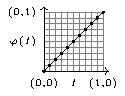
\includegraphics[width=\textwidth]{figures/dyn-prog-full-disc-id/fig.pdf}
        \caption{}
        \label{fig:dyn-prog-full-disc-id}
    \end{subfigure}
    \hfill
    \begin{subfigure}[b]{0.45\textwidth}
        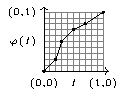
\includegraphics[width=\textwidth]{figures/dyn-prog-full-disc/fig.pdf}
        \caption{}
        \label{fig:dyn-prog-full-disc}
    \end{subfigure}
    \caption[Reparameterization with Full Discretization]{Reparameterization using full discretization. (a) the identity transformation (no change to the original parameterization), and (b) a reparameterized path.}
    \label{fig:dyn-prog}
\end{figure}

The condition \(k < i\) and \(l < j\) ensures the transformation proceeds positively, avoiding loops and maintaining the orientation of \(q_2\).
\subsection{Neighborhood Search Strategy}
\label{subsec:neighborhood-search-strategy}

Despite its straightforward implementation, this method presents significant computational challenges. For a grid comprising \(n \times n\) points, the process involves solving \(n^2\) subproblems, each requiring \(\mathcal{O}(n^2)\) operations. This leads to a total computational complexity of \(\mathcal{O}(n^4)\), making the method computationally intensive, especially for large-scale applications.

To mitigate these computational demands, a strategic limitation of the search area for each subproblem is proposed, as illustrated in Figure \ref{fig:dyn-prog-full-disc-search}. The size of this area must be adaptable based on the grid's dimensions; a fixed size may excessively restrict path movement in smaller grids. Employing this neighborhood search strategy significantly reduces computational cost to \(\mathcal{O}(n^2 |\mathcal{N}(n)|)\), where \(|\mathcal{N}(n)|\) indicates the search area's size.

\begin{figure}
    \centering
    \begin{subfigure}{.3\textwidth}
        \centering
        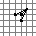
\includegraphics[width=\linewidth]{figures/dyn-prog-full-disc-search-2/fig.pdf}
        \caption{}
        \label{fig:dyn-prog-full-disc-search-2}
    \end{subfigure}%
    \begin{subfigure}{.3\textwidth}
        \centering
        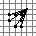
\includegraphics[width=\linewidth]{figures/dyn-prog-full-disc-search-3/fig.pdf}
        \caption{}
        \label{fig:dyn-prog-full-disc-search-3}
    \end{subfigure}%
    \begin{subfigure}{.3\textwidth}
        \centering
        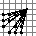
\includegraphics[width=\linewidth]{figures/dyn-prog-full-disc-search-4/fig.pdf}
        \caption{}
        \label{fig:dyn-prog-full-disc-search-4}
    \end{subfigure}
    \caption[Search Areas for Fully Discretized Reparameterization]{Visualization of limited search areas for different values of search depth \(m\): (a) \(m = 2\), (b) \(m = 3\), and (c) \(m = 4\). These figures demonstrate how increasing search depths expand the area being considered, thereby influencing the computational cost and efficiency of the reparameterization process.}    
    \label{fig:dyn-prog-full-disc-search}
\end{figure}

The limited search area is defined as follows:
\begin{equation}
    \mathcal{N}_{(i, j)}(n) = \{(k, l) \mid i-m \leq k < i, \, j-m < l < j, \, \gcd(i - k, j - l) = 1\},
    \label{eq:search-area}
\end{equation}
where \(m = f(n) \in \mathbb{N}^+\) is a function of the grid size \(n\) that determines the extent of the search area. The condition \(\gcd(i - k, j - l) = 1\) ensures that the path does not traverse any intermediate grid points, maintaining a direct route between the specified points and improving the computational efficiency of the process.

To illustrate the implementation of this strategy, we present the pseudocode for the optimal reparameterization process using dynamic programming in Algorithm \ref{alg:optimal-reparam-dp}. This algorithm aligns two curves by optimizing the parameterizations of the second curve, reducing the computational complexity through the limited search area defined earlier.

\begin{algorithm}
    \caption{Optimal Reparameterization via Dynamic Programming}
    \label{alg:optimal-reparam-dp}
    \begin{algorithmic}[1]
    \Require $c_1, c_2$: Curves, $I_1, I_2 \in \mathbb{R}$: Initial parameterizations
    \Function{OptimizeReparam}{$c_1, c_2, I_1, I_2$}
        \State $(I, c_1', c_2') \gets \text{AlignCurves}(c_1, c_2, I_1, I_2)$
        \State $(c_{1,e}', c_{2,e}') \gets \text{MoveStartToIdentity}(c_1', c_2')$ \Comment{\eqref{eq:maurer-cartan-gl}}
        \State $(q_1, q_2) \gets \text{vee}(\text{SRVT}(c_{1,e}', c_{2,e}'))$ \Comment{\eqref{eq:srvt-discrete}, \eqref{eq:vee_SO3}, \eqref{eq:vee_SE3}}
        \State $A, P \gets \text{ComputeCostMatrix}(q_1, q_2)$  \Comment{\eqref{eq:cost-matrix}}
        \State $\text{path} \gets \text{TraceOptimalPath}(P)$ 
        \State $I_{2, opt} \gets \text{LinearInterpolate}(\text{path}_x, \text{path}_y)(I_2)$ 
        \State $c_{2, opt} \gets \text{Interpolate}(I_{2}, I_{2, opt})(c_2)$  \Comment{\eqref{eq:interpolation-discrete}}
        \State \Return $(c_{2, opt}, I_{2, opt})$
    \EndFunction
    \end{algorithmic}
\end{algorithm}

The algorithm detailed in Algorithm \ref{alg:calculate-cost-parent} calculates the cost and parent matrices used in the dynamic programming approach. By leveraging the limited search area, it ensures efficient computation of the optimal path.

\begin{algorithm}
    \caption{Calculate Cost and Parent Matrices for Dynamic Programming}
    \label{alg:calculate-cost-parent}
    \begin{algorithmic}[1]
    \Require $I \in \mathbb{R}^n$: Grid points
    \Require $q_0, q_1 \in \mathbb{R}^{n-1}$: Values defined on the domain of $I$
    \Require $\text{depth} \in \mathbb{N}^+$: Depth of the search area
    \Function{calculateCostMatrixAndParent}{$I, q_0, q_1, \text{depth}$}
        \State $n \gets \text{length}(I)$
        \State $A \gets \text{matrix\_of\_infinity}(n, n)$ \Comment{Initialize cost matrix to a large value}
        \State $P \gets \text{empty matrix}(n, n)$ \Comment{Initialize parent matrix}
        
        \State $A[0, 0] \gets 0$ \Comment{Set initial cost to zero}
        \State $P[0, 0] \gets \text{None}$ \Comment{No predecessor for initial condition}
        
        \For{$i \gets 0$ \textbf{to} $n-1$}
            \For{$j \gets 0$ \textbf{to} $n-1$}
                \State $\text{preds} \gets \text{findPreds}(i, j, \text{depth})$ \Comment{\eqref{eq:search-area}}
                \For{$\text{pred} \in \text{preds}$}
                    \State $\text{cost\_to\_pred} \gets \text{localCost}(i, j, \text{pred}, q_0, q_1)$ 
                    \Comment{\eqref{eq:local-cost-functional}, \eqref{eq:local-cost-functional-SE3}}
                    \State $\text{cost} \gets \text{cost\_to\_pred} + A[\text{pred}]$ \Comment{\eqref{eq:cost-matrix}}
                    \If{$\text{cost} < A[i, j]}$
                        \State $A[i, j] \gets \text{cost}$
                        \State $P[i, j] \gets \text{pred}$
                    \EndIf
                \EndFor
            \EndFor
        \EndFor
    
        \State \Return $P, A$
    \EndFunction
    \end{algorithmic}
\end{algorithm}
\subsection{Synthetic Data Generation}
\label{subsec:synthetic-data-generation}

In this subsection, we outline the process of generating synthetic data for numerical analysis. This synthetic data is critical for evaluating our reparameterization framework. We generate data by solving differential equations with different parameterizations. The synthetic data includes trajectories, parameterizations, and curves for different groups such as \(\mathrm{SO}(3)\), \(\mathrm{SE}(3)\), \(\mathrm{SO}(3)^3\), and \(\mathrm{SE}(3)^3\). These elements are used later in our numerical analysis.

\subsubsection{Generating Synthetic Trajectories}
\label{subsubsec:synthetic-trajectories-generation}

To generate synthetic trajectories, we model the system using the differential equation:
\begin{equation}
    \frac{d}{dt} g(t) = g(t) \hat{u}(t), \quad t \in [0, 1],
    \label{eq:diff-eq-synthetic}
\end{equation}
where \( g(t) \in \mathrm{SO}(3) \) or \( \mathrm{SE}(3) \), and \(\hat{u}(t)\) is the hat map of \(u(t)\). We assume an initial value \( g(0) = e \) (the identity element). By varying \(\hat{u}(t)\) with different parameterizations, we synthesize diverse datasets. The trajectories are approximated using the fourth-order Runge-Kutta (RK4) method \cite{rungeUeberNumerischeAufloesung1895,butcherCoefficientsStudyRungeKutta1963} over discrete time intervals.

For \(\mathrm{SO}(3)\), we set \(u(t) = \omega_i(t) \in \mathbb{R}^3\). For \(\mathrm{SE}(3)\), we set \(u(t) = \xi_i(t) = [\omega_i(t), v_i(t)]^T \in \mathbb{R}^6\), which is mapped to the corresponding Lie algebra via \eqref{eq:hat_SO3} and \eqref{eq:hat_SE3}.

To demonstrate the generation of synthetic data for Cartesian curves, \(n = 3\) is chosen. For either \(\mathrm{SO}(3)^3\) or \(\mathrm{SE}(3)^3\), we define three different functions \(u(t)\). Thus, solving \eqref{eq:diff-eq-synthetic} generates three synthetic trajectories over discrete time intervals.

We define nine \(\omega_i(t)\) and nine \(v_i(t)\) to generate the rotational and translational components, respectively, used for \(u(t)\). The rotational functions are defined in \eqref{eq:synthetic-data-rotation}, and the translational functions are defined in \eqref{eq:synthetic-data-translation}.

\begin{equation}
    \begin{aligned}
        \omega_1(t) &= 
            [2 \sin(3t) \exp(t), 4 \cos(3t), 3t \sin(t) \cos(t)]^T \\
        \omega_2(t) &= 
            [3t, 4 \sin(10t), 3t \sin(t) \cos(t)]^T \\
        \omega_3(t) &= 
            [4t^2, 5 \sin(4t) \sin(6t), 3t \cos(t)]^T \\
        \omega_4(t) &= 
            [3 \sin(2t) \exp(-t), 5 \cos(2t), 4t \sin(t) \cos(t)]^T \\
        \omega_5(t) &= 
            [t^3, 5 \sin(5t), 2t \sin(t) \sin(t)]^T \\
        \omega_6(t) &= 
            [2t^2, 3 \sin(6t) \cos(t), 5t \cos(t) \cos(t)]^T \\
        \omega_7(t) &= 
            [-1, 6 \sin(3t), 3t \sin(t)]^T \\
        \omega_8(t) &= 
            [t^2, 4 \cos(3t), t \sin(t)]^T \\
        \omega_9(t) &= 
            [3t, 5 \sin(2t), 2t \cos(t)]^T
    \end{aligned}
    \label{eq:synthetic-data-rotation}
\end{equation}

\begin{equation}
    \begin{aligned}
        v_1(t) &= 
        [3t \sin(t) \cos(t), t, \cos(t), \sin(3t)]^T \\
        v_2(t) &=
        [\sin(2t), \cos(3t), \exp(t)]^T \\
        v_3(t) &=
        [\cos(t) \cos(3t), \sin(4t), \cos(2t)]^T \\
        v_4(t) &=
        [t^2, \sin(t^2), \exp(-t)]^T \\
        v_5(t) &=
        [\cos(2t), \log(t + 1), t]^T \\
        v_6(t) &=
        [\sin(t) \cos(t), t^3, \sin(t^3)]^T \\
        v_7(t) &=
        [\cos(5t), \exp(t/2), t \sin(t)]^T \\
        v_8(t) &=
        [\sin(2t), t \exp(-t), \cos(t^2)]^T \\
        v_9(t) &=
        [t^2 \cos(t), \sin(t^2), -0.5]^T
    \end{aligned}
    \label{eq:synthetic-data-translation}
\end{equation}

By solving \eqref{eq:diff-eq-synthetic} with \(u(t) = \omega_i(t)\), for \(i = 1, 2, \dots, 9\) over equidistant points on \([0,1]\), we obtain the rotational trajectories depicted in Figure \ref{fig:synthetic-rotation}. Similarly, by solving \eqref{eq:diff-eq-synthetic} with \(u(t) = \xi_i(t)\), for \(i = 1, 2, \dots, 9\) over equidistant points on \([0,1]\), and extracting the positions, we generate the translation plot shown in Figure \ref{fig:synthetic-translation}. These plots provide a clear visual representation of the varied rotational and translational paths used later in the analysis. The rotations are plotted on spheres, representing pure rotational movements.

\newpage
\begin{figure}
    \centering
    \foreach \i in {1,...,9} {
        \begin{subfigure}{0.26\textwidth}
            \includegraphics[width=\textwidth]{figures/syntetic_data/SO3_fig\i.png}
            \caption{}
            \label{fig:synthetic-SO3-fig\i}
        \end{subfigure}
        \ifnum\i=3
            \par\medskip % start a new line after the third subfigure
        \fi
        \ifnum\i=6
            \par\medskip % start a new line after the sixth subfigure
        \fi
    }
    \caption[Visualization of Rotations from Synthetic Data]{Rotations generated from synthetic data using \eqref{eq:synthetic-data-rotation}. Each subfigure (a-i) shows the rotation of the initial vector \([0, 0, 1]\) governed by \eqref{eq:diff-eq-synthetic} with \(\hat{u}(t) = \hat{\omega}_i(t)\), evaluated over \([0, 1]\) with 100 time points. Subfigures (a-i) correspond to \(i = 1\) to \(i = 9\), respectively.}
    \label{fig:synthetic-rotation}
\end{figure}

\newpage
\begin{figure}
    \centering
    \foreach \i in {1,2,3,4,5,6,7,8,9} {
        \begin{subfigure}[b]{0.3\textwidth}
            \centering
            \begin{tikzpicture}
                \begin{axis}[
                    height=4.5cm,
                    width=5cm,
                    xlabel=$x$, 
                    ylabel=$y$, 
                    zlabel=$z$,
                    ytick=\empty,
                    xtick=\empty,
                    ztick=\empty
                ]
                    \addplot3+[
                        mark options={red, mark size=0.5pt},
                        only marks,
                    ] table [col sep=comma, x=x, y=y, z=z] {figures/syntetic_data/SE3_t_\i.csv};
                \end{axis}
            \end{tikzpicture}
            \caption{}
        \end{subfigure}
        \ifnum\i=3 \hspace{0pt}\par\fi % Line break after every third subfigure
        \ifnum\i=6 \hspace{0pt}\par\fi
    }
    \caption[Visualization of Translations from Synthetic Data]{Translation part of the \(\mathrm{SE}(3)\) elements generated from synthetic data by solving \eqref{eq:diff-eq-synthetic} with the functions defined in \eqref{eq:synthetic-data-rotation} and \eqref{eq:synthetic-data-translation}. Each subfigure (a-i) illustrates the translation governed by \eqref{eq:diff-eq-synthetic} with \(\hat{u}(t) = \hat{\xi}_i(t)\), evaluated over \([0, 1]\) with 100 time points. Subfigures (a-i) correspond to \(i = 1\) to \(i = 9\), respectively.}
    \label{fig:synthetic-translation}
\end{figure}

\FloatBarrier
\subsubsection{Generate Synthetic Parameterizations}
\label{subsubsec:generate-synthetic-parameterizations}

We generate three distinct synthetic parameterizations, each created by \(\varphi(x) \in \mathrm{Diff}^+([0,1])\):

\begin{equation}
    \varphi(x) = x + F(x),
\end{equation}
where \(\varphi'(x) = 1 + F'(x) > 0\). The function \(F(x)\) is constructed using an orthogonal sine basis function \(\psi_n(x)\):

\begin{equation}
    \psi_n(x) = \frac{\sin(n \pi x)}{n \pi}, \quad n \in \mathbb{N}.
\end{equation}

These basis functions are orthogonal over \([0, 1]\) and vanish at the endpoints, making them suitable for weighted sums. Consequently, \(F(x)\) is represented as:

\begin{equation}
    F(x) = \sum_{n=1}^{M} w_n \psi_n(x) = \sum_{n=1}^{M} w_n \frac{\sin(n \pi x)}{n \pi},
\end{equation}
where \(w_n\) are the weights associated with each basis function. The derivative \(F'(x)\) is:

\begin{equation}
    F'(x) = \sum_{n=1}^{M} w_n \cos(n \pi x).
\end{equation}

Since each cosine term is bounded by 1, the derivative \(F'(x)\) satisfies:

\begin{equation}
    |F'(x)| \leq \|\mathbf{w}\|_1.
\end{equation}

Therefore, the derivative of \(\varphi(x)\) is:

\begin{equation}
    \varphi'(x) = 1 + \sum_{n=1}^{M} w_n \cos(n \pi x).
\end{equation}

To ensure \(\varphi'(x) > 0\), we scale \(F(x)\) by a factor \(\frac{1 - \epsilon}{\|\mathbf{w}\|_1}\), where \(\epsilon\) is a small positive number. This guarantees that the sum of the cosine terms is less than 1, ensuring \(\varphi'(x) > 0\):

\begin{equation}
    1 + \sum_{n=1}^{M} w_n \frac{1 - \epsilon}{\|\mathbf{w}\|_1} \cos(n \pi x) > 0.
\end{equation}

The synthetic parameterizations generated using this method are illustrated in Figure \ref{fig:synthetic-parameterizations}. For this, we set \(M = 4\), initialize the weights \(w_n\) with a normal distribution \(\mathcal{N}(0, 2)\), and use 100 equidistant steps with a tolerance of \(\epsilon = 10^{-8}\).

\begin{figure}
    \begin{tikzpicture}
        \begin{axis}[
            width=0.7\textwidth,
            height=0.5\textwidth,
            xlabel={\( x \)},
            ylabel={\( \varphi(x) \)},
            grid=major,
            grid style={dashed,gray!30},
            legend style={at={(1.05,0.5)}, anchor=west},
            line width=1pt,
            xmin=0, xmax=1,
            ymin=0, ymax=1
        ]
        \addplot [smooth, thick, red] table [x=x, y=varphi_1, col sep=comma] {figures/syntetic_data/parameterization/varphi_1.csv};
        \addlegendentry{\( \varphi_1 \)}
        \addplot [smooth, thick, blue] table [x=x, y=varphi_2, col sep=comma] {figures/syntetic_data/parameterization/varphi_2.csv};
        \addlegendentry{\( \varphi_2 \)}
        \addplot [smooth, thick, orange] table [x=x, y=varphi_3, col sep=comma] {figures/syntetic_data/parameterization/varphi_3.csv};
        \addlegendentry{\( \varphi_3 \)}
        \end{axis}
    \end{tikzpicture}    
    \caption[Visualization of the Synthetic Parameterizations]{Visualization of three distinct synthetic parameterizations generated by setting \(M = 4\), initializing the weights \(w_n\) with a normal distribution \(\mathcal{N}(0, 2)\), and using 100 equidistant steps with a tolerance of \(\epsilon = 10^{-8}\).}
    \label{fig:synthetic-parameterizations}
\end{figure}

\FloatBarrier
\subsubsection{Generate Synthetic Curves}
\label{subsubsec:synthetic-curves}

To evaluate our reparameterization framework, we generate synthetic curves by solving Equation \eqref{eq:diff-eq-synthetic} with the parameterizations \(\varphi_1, \varphi_2, \varphi_3\) described in Section \ref{subsubsec:generate-synthetic-parameterizations}, as well as an equidistant parameterization. This differential equation is solved using the functions defined in Equations \eqref{eq:synthetic-data-rotation} and \eqref{eq:synthetic-data-translation}, which provide \(u(t) = \omega_i(t)\) for \(\mathrm{SO}(3)\) elements and \(u(t) = \xi_i(t) = [\omega_i(t), v_i(t)]^T\) for \(\mathrm{SE}(3)\) elements, where \(i = 1,2,3\). This process creates single-element and three-element Cartesian curves, with each group comprising three shapes, each represented under four different parameterizations, yielding twelve curves per group.

For multi-component groups \(\mathrm{SO}(3)^3\) and \(\mathrm{SE}(3)^3\), we define composite parameters:
\begin{gather}
    \omega_{i, i+1, i+2} = [\omega_i, \omega_{i+1}, \omega_{i+2}], \nonumber \\
    \xi_{i, i+1, i+2} = \left[ \xi_i, \xi_{i+1}, \xi_{i+2} \right] = \left[ [\omega_i, v_i], [\omega_{i+1}, v_{i+1}], [\omega_{i+2}, v_{i+2}] \right] 
\end{gather}
for \(i \in \{1, 4, 7\}\).

The idea is to create three interconnected curves that together form a single composite curve. These parameters are used to solve the differential equation under the same parameterizations, generating twelve curves per group. Each group of four curves shares identical geometric shapes, differentiated by parameterization.

The notation for the curves is as follows: single-element curves are denoted \(c_i^j\), where \(i\) indicates the parameter used (\(\omega_i\) or \(\xi_i = [\omega_i, v_i]\)) and \(j\) the specific parameterization (\(\varphi_j\)). Curves generated using the equidistant parameterization are denoted as \(c_i^{\text{eq}}\). Cartesian curves are expressed as \(c_{i, i+1, i+2}^j\) for individual parameterizations and \(c_{i, i+1, i+2}^{\text{eq}}\) for the equidistant parameterization.

\subsection{Numerical Analysis}
\label{sec:numerical-reparameterization}

In this subsection we will use the data in \ref{subsec:synthetic-data-generation} perform reparameterization, classification and measure performance in terms of accuracy and computation time as the search size increases.

\FloatBarrier
\subsubsection{Reparameterization of Curves}
\label{subsec:reparameterization-curves}

In this subsection, we evaluate the reparameterization framework using synthetic curves generated previously (Section \ref{subsec:synthetic-data-generation}). The goal is to reparameterize the equidistantly parameterized curves \(c_i^\text{eq}\) into the curves \(c_i^j\) for \(i \in \{1, 2, 3\}\) and \(c_{i,i+1,i+2}^\text{eq}\) into the curves \(c_{i,i+1,i+2}^j\) for \(i \in \{1, 4, 7\}\), for all parameterizations \(j \in \{1, 2, 3\}\). This evaluation checks whether we can find the optimal reparameterization when the shapes are the same, demonstrating that we can effectively remove the effects of parameterization through reparameterization. It does not, however, determine whether we can differentiate between different shapes.

The objective is to find the optimal reparameterization \(\hat{\varphi}_j\) that approximates \(\varphi_j\). The relationship between the curves is given by:
\begin{equation}
    c_i^j = c_i^\text{eq} \circ \varphi_j
\end{equation}

Hence, each curve \(c_i^j\) is obtained by composing the equidistant curve \(c_i^\text{eq}\) with one of the parameterizations \(\varphi_1, \varphi_2\), or \(\varphi_3\). Thus, to find the optimal reparameterization \(\hat{\varphi}_j\), we minimize the distance \(d_{\mathcal{S}_*}\) between \(c_i^j\) and \(c_i^{\text{eq}}\):
\begin{equation}
    d_{\mathcal{S}_*}(c_i^j, c_i^{\text{eq}}) = \min_{\hat{\varphi}_j} d_{\mathcal{P}_*}(c_i^{\text{eq}} \circ \varphi_j, c_i^{\text{eq}} \circ \hat{\varphi}_j)
\end{equation}

This minimization process helps to determine \(\hat{\varphi}_j\) such that \(\hat{\varphi}_j \approx \varphi_j\), indicating that the reparameterization framework can effectively approximate the original parameterizations.

The results after reparameterization for the curves in \(\mathrm{SO}(3)\), \(\mathrm{SE}(3)\), \(\mathrm{SO}(3)^3\), and \(\mathrm{SE}(3)^3\) are presented in Figures \ref{fig:reparameterization-SO3}, \ref{fig:reparameterization-SE3}, \ref{fig:reparameterization-SO3-3}, and \ref{fig:reparameterization-SE3-3}, respectively.

\begin{figure}
    \begin{tikzpicture}
        \begin{axis}[
            width=0.85\textwidth,
            height=0.55\textwidth,
            xlabel={\( x \)},
            ylabel={\( \varphi(x) \)},
            grid=major,
            grid style={dashed,gray!30},
            legend style={at={(1.05,0.5)}, anchor=west},
            line width=1pt,
            xmin=0, xmax=1,
            ymin=0, ymax=1,
        ]
        \addplot [thin, red, solid] table [x=x, y=varphi_1, col sep=comma] {figures/syntetic_data/parameterization/varphi_1.csv};
        \addlegendentry{\( \varphi_1\)}

        \addplot [thin, blue, solid] table [x=x, y=varphi_2, col sep=comma] {figures/syntetic_data/parameterization/varphi_2.csv};
        \addlegendentry{\( \varphi_2\)}

        \addplot [thin, green, solid] table [x=x, y=varphi_3, col sep=comma] {figures/syntetic_data/parameterization/varphi_3.csv};
        \addlegendentry{\( \varphi_3\)}


        \addplot [red, dashed] table [x=x, y=g0, col sep=comma] {figures/syntetic_data/reparameterization_SO3/df_varphi_1.csv};
        \addlegendentry{\( \hat \varphi_{1}^{1}\)}

        \addplot [red, dotted] table [x=x, y=g1, col sep=comma] {figures/syntetic_data/reparameterization_SO3/df_varphi_1.csv};
        \addlegendentry{\( \hat \varphi_{1}^{2}\)}

        \addplot [red, dashdotted] table [x=x, y=g2, col sep=comma] {figures/syntetic_data/reparameterization_SO3/df_varphi_1.csv};
        \addlegendentry{\( \hat \varphi_{1}^{3}\)}

        \addplot [blue, dashed] table [x=x, y=g0, col sep=comma] {figures/syntetic_data/reparameterization_SO3/df_varphi_2.csv};
        \addlegendentry{\( \hat \varphi_{2}^{1}\)}

        \addplot [blue, dotted] table [x=x, y=g1, col sep=comma] {figures/syntetic_data/reparameterization_SO3/df_varphi_2.csv};
        \addlegendentry{\( \hat \varphi_{2}^{2}\)}

        \addplot [blue, dashdotted] table [x=x, y=g2, col sep=comma] {figures/syntetic_data/reparameterization_SO3/df_varphi_2.csv};
        \addlegendentry{\( \hat \varphi_{2}^{3}\)}

        \addplot [green, dashed] table [x=x, y=g0, col sep=comma] {figures/syntetic_data/reparameterization_SO3/df_varphi_3.csv};
        \addlegendentry{\( \hat \varphi_{3}^{1}\)}

        \addplot [green, dotted] table [x=x, y=g1, col sep=comma] {figures/syntetic_data/reparameterization_SO3/df_varphi_3.csv};
        \addlegendentry{\( \hat \varphi_{3}^{2}\)}

        \addplot [green, dashdotted] table [x=x, y=g2, col sep=comma] {figures/syntetic_data/reparameterization_SO3/df_varphi_3.csv};
        \addlegendentry{\( \hat \varphi_{3}^{3}\)}

        \end{axis}
    \end{tikzpicture}    
    \caption[Reparameterization of curves in \(\mathrm{SO}(3)\)]{Comparison of reparameterized curves \(\hat{\varphi}_j^i\) with the analytical parameterizations \(\varphi_j\) for curves in \(\mathrm{SO}(3)\). The curves \(c_i^{\text{eq}}\) have been fitted to \(c_i^j\) for \(j = 1, 2, 3\), and for all shapes \(i = 1, 2, 3\). Optimal reparameterizations are indicated by \(\hat{\varphi}_i^j\) being close to \(\varphi_j\).}
    \label{fig:reparameterization-SO3}
\end{figure}

\begin{figure}
    \begin{tikzpicture}
        \begin{axis}[
            width=0.85\textwidth,
            height=0.55\textwidth,
            xlabel={\( x \)},
            ylabel={\( \varphi(x) \)},
            grid=major,
            grid style={dashed,gray!30},
            legend style={at={(1.05,0.5)}, anchor=west},
            line width=1pt,
            xmin=0, xmax=1,
            ymin=0, ymax=1,
        ]
        \addplot [thin, red, solid] table [x=x, y=varphi_1, col sep=comma] {figures/syntetic_data/parameterization/varphi_1.csv};
        \addlegendentry{\( \varphi_1\)}

        \addplot [thin, blue, solid] table [x=x, y=varphi_2, col sep=comma] {figures/syntetic_data/parameterization/varphi_2.csv};
        \addlegendentry{\( \varphi_2\)}

        \addplot [thin, green, solid] table [x=x, y=varphi_3, col sep=comma] {figures/syntetic_data/parameterization/varphi_3.csv};
        \addlegendentry{\( \varphi_3\)}

        \addplot [red, dashed] table [x=x, y=g0, col sep=comma] {figures/syntetic_data/reparameterization_SE3/df_varphi_1.csv};
        \addlegendentry{\( \hat \varphi_{1}^1\)}

        \addplot [red, dotted] table [x=x, y=g1, col sep=comma] {figures/syntetic_data/reparameterization_SE3/df_varphi_1.csv};
        \addlegendentry{\( \hat \varphi_{1}^2\)}

        \addplot [red, dashdotted] table [x=x, y=g2, col sep=comma] {figures/syntetic_data/reparameterization_SE3/df_varphi_1.csv};
        \addlegendentry{\( \hat \varphi_{1}^3\)}

        \addplot [blue, dashed] table [x=x, y=g0, col sep=comma] {figures/syntetic_data/reparameterization_SE3/df_varphi_2.csv};
        \addlegendentry{\( \hat \varphi_{2}^1\)}

        \addplot [blue, dotted] table [x=x, y=g1, col sep=comma] {figures/syntetic_data/reparameterization_SE3/df_varphi_2.csv};
        \addlegendentry{\( \hat \varphi_{2}^2\)}

        \addplot [blue, dashdotted] table [x=x, y=g2, col sep=comma] {figures/syntetic_data/reparameterization_SE3/df_varphi_2.csv};
        \addlegendentry{\( \hat \varphi_{2}^3\)}

        \addplot [green, dashed] table [x=x, y=g0, col sep=comma] {figures/syntetic_data/reparameterization_SE3/df_varphi_3.csv};
        \addlegendentry{\( \hat \varphi_{3}^1\)}

        \addplot [green, dotted] table [x=x, y=g1, col sep=comma] {figures/syntetic_data/reparameterization_SE3/df_varphi_3.csv};
        \addlegendentry{\( \hat \varphi_{3}^2\)}

        \addplot [green, dashdotted] table [x=x, y=g2, col sep=comma] {figures/syntetic_data/reparameterization_SE3/df_varphi_3.csv};
        \addlegendentry{\( \hat \varphi_{3}^3\)}

        \end{axis}
    \end{tikzpicture}    
    \caption[Reparameterization of curves in \(\mathrm{SE}(3)\)]{Comparison of reparameterized curves \(\hat{\varphi}_j^i\) with the analytical parameterizations \(\varphi_j\) for curves in \(\mathrm{SE}(3)\). The curves \(c_i^{\text{eq}}\) have been fitted to \(c_i^j\) for \(j = 1, 2, 3\), and for all shapes \(i = 1, 2, 3\). Optimal reparameterizations are indicated by \(\hat{\varphi}_j^i\) being close to \(\varphi_j\).}
    \label{fig:reparameterization-SE3}
\end{figure}

\begin{figure}
    \begin{tikzpicture}
        \begin{axis}[
            width=0.8\textwidth,
            height=0.55\textwidth,
            xlabel={\( x \)},
            ylabel={\( \varphi(x) \)},
            grid=major,
            grid style={dashed,gray!30},
            legend style={at={(1.05,0.5)}, anchor=west},
            line width=1pt,
            xmin=0, xmax=1,
            ymin=0, ymax=1,
        ]
        \addplot [thin, red, solid] table [x=x, y=varphi_1, col sep=comma] {figures/syntetic_data/parameterization/varphi_1.csv};
        \addlegendentry{\( \varphi_1\)}

        \addplot [thin, blue, solid] table [x=x, y=varphi_2, col sep=comma] {figures/syntetic_data/parameterization/varphi_2.csv};
        \addlegendentry{\( \varphi_2\)}

        \addplot [thin, green, solid] table [x=x, y=varphi_3, col sep=comma] {figures/syntetic_data/parameterization/varphi_3.csv};
        \addlegendentry{\( \varphi_3\)}


        \addplot [red, dashed] table [x=x, y=g0, col sep=comma] {figures/syntetic_data/reparameterization_SO3_3/df_varphi_1.csv};
        \addlegendentry{\( \hat \varphi_{1}^{(1,2,3)}\)}

        \addplot [red, dotted] table [x=x, y=g1, col sep=comma] {figures/syntetic_data/reparameterization_SO3_3/df_varphi_1.csv};
        \addlegendentry{\( \hat \varphi_{1}^{(4,5,6)}\)}

        \addplot [red, dashdotted] table [x=x, y=g2, col sep=comma] {figures/syntetic_data/reparameterization_SO3_3/df_varphi_1.csv};
        \addlegendentry{\( \hat \varphi_{1}^{(7,8,9)}\)}

        \addplot [blue, dashed] table [x=x, y=g0, col sep=comma] {figures/syntetic_data/reparameterization_SO3_3/df_varphi_2.csv};
        \addlegendentry{\( \hat \varphi_{2}^{(1,2,3)}\)}

        \addplot [blue, dotted] table [x=x, y=g1, col sep=comma] {figures/syntetic_data/reparameterization_SO3_3/df_varphi_2.csv};
        \addlegendentry{\( \hat \varphi_{2}^{(4,5,6)}\)}

        \addplot [blue, dashdotted] table [x=x, y=g2, col sep=comma] {figures/syntetic_data/reparameterization_SO3_3/df_varphi_2.csv};
        \addlegendentry{\( \hat \varphi_{2}^{(7,8,9)}\)}

        \addplot [green, dashed] table [x=x, y=g0, col sep=comma] {figures/syntetic_data/reparameterization_SO3_3/df_varphi_3.csv};
        \addlegendentry{\( \hat \varphi_{3}^{(1,2,3)}\)}

        \addplot [green, dotted] table [x=x, y=g1, col sep=comma] {figures/syntetic_data/reparameterization_SO3_3/df_varphi_3.csv};
        \addlegendentry{\( \hat \varphi_{3}^{(4,5,6)}\)}

        \addplot [green, dashdotted] table [x=x, y=g2, col sep=comma] {figures/syntetic_data/reparameterization_SO3_3/df_varphi_3.csv};
        \addlegendentry{\( \hat \varphi_{3}^{(7,8,9)}\)}
        \end{axis}
    \end{tikzpicture}    
    \caption[Reparameterization of curves in \(\mathrm{SO}(3)^3\)]{Comparison of reparameterized curves \(\hat{\varphi}_j^{i,i+1,i+2}\) with the analytical parameterizations \(\varphi_j\) for curves in \(\mathrm{SE}(3)\). The curves \(c_{i,i+1,i+2}^{\text{eq}}\) have been fitted to \(c_{i,i+1,i+2}^j\) for \(i \in \{1, 2, 3\}\), and for all shapes \(i \in \{1, 4, 7\}\). Optimal reparameterizations are indicated by \(\hat{\varphi}_j^{i,i+1,i+2}\) being close to \(\varphi_j\).}
    \label{fig:reparameterization-SO3-3}
\end{figure}

\begin{figure}
    \begin{tikzpicture}
        \begin{axis}[
            width=0.8\textwidth,
            height=0.55\textwidth,
            xlabel={\( x \)},
            ylabel={\( \varphi(x) \)},
            grid=major,
            grid style={dashed,gray!30},
            legend style={at={(1.05,0.5)}, anchor=west},
            line width=1pt,
            xmin=0, xmax=1,
            ymin=0, ymax=1,
        ]
        \addplot [thin, red, solid] table [x=x, y=varphi_1, col sep=comma] {figures/syntetic_data/parameterization/varphi_1.csv};
        \addlegendentry{\( \varphi_1\)}

        \addplot [thin, blue, solid] table [x=x, y=varphi_2, col sep=comma] {figures/syntetic_data/parameterization/varphi_2.csv};
        \addlegendentry{\( \varphi_2\)}

        \addplot [thin, green, solid] table [x=x, y=varphi_3, col sep=comma] {figures/syntetic_data/parameterization/varphi_3.csv};
        \addlegendentry{\( \varphi_3\)}



        \addplot [red, dashed] table [x=x, y=g0, col sep=comma] {figures/syntetic_data/reparameterization_SE3_3/df_varphi_1.csv};
        \addlegendentry{\( \hat \varphi_{1}^{(1,2,3)}\)}

        \addplot [red, dotted] table [x=x, y=g1, col sep=comma] {figures/syntetic_data/reparameterization_SE3_3/df_varphi_1.csv};
        \addlegendentry{\( \hat \varphi_{1}^{(4,5,6)}\)}

        \addplot [red, dashdotted] table [x=x, y=g2, col sep=comma] {figures/syntetic_data/reparameterization_SE3_3/df_varphi_1.csv};
        \addlegendentry{\( \hat \varphi_{1}^{(7,8,9)}\)}

        \addplot [blue, dashed] table [x=x, y=g0, col sep=comma] {figures/syntetic_data/reparameterization_SE3_3/df_varphi_2.csv};
        \addlegendentry{\( \hat \varphi_{2}^{(1,2,3)}\)}

        \addplot [blue, dotted] table [x=x, y=g1, col sep=comma] {figures/syntetic_data/reparameterization_SE3_3/df_varphi_2.csv};
        \addlegendentry{\( \hat \varphi_{2}^{(4,5,6)}\)}

        \addplot [blue, dashdotted] table [x=x, y=g2, col sep=comma] {figures/syntetic_data/reparameterization_SE3_3/df_varphi_2.csv};
        \addlegendentry{\( \hat \varphi_{2}^{(7,8,9)}\)}

        \addplot [green, dashed] table [x=x, y=g0, col sep=comma] {figures/syntetic_data/reparameterization_SE3_3/df_varphi_3.csv};
        \addlegendentry{\( \hat \varphi_{3}^{(1,2,3)}\)}

        \addplot [green, dotted] table [x=x, y=g1, col sep=comma] {figures/syntetic_data/reparameterization_SE3_3/df_varphi_3.csv};
        \addlegendentry{\( \hat \varphi_{3}^{(4,5,6)}\)}

        \addplot [green, dashdotted] table [x=x, y=g2, col sep=comma] {figures/syntetic_data/reparameterization_SE3_3/df_varphi_3.csv};
        \addlegendentry{\( \hat \varphi_{3}^{(7,8,9)}\)}

        \end{axis}
    \end{tikzpicture}    
    \caption[Reparameterization of curves in \(\mathrm{SE}(3)^3\)]{Comparison of reparameterized curves \(\hat{\varphi}_j^{i,i+1,i+2}\) with the analytical parameterizations \(\varphi_j\) for curves in \(\mathrm{SE}(3)\). The curves \(c_{i,i+1,i+2}^{\text{eq}}\) have been fitted to \(c_{i,i+1,i+2}^j\) for \(j \in \{1, 2, 3\}\), and for all shapes \(i \in \{1, 4, 7\}\). Optimal reparameterizations are indicated by \(\hat{\varphi}_j^{i,i+1,i+2}\) being close to \(\varphi_j\).}
    \label{fig:reparameterization-SE3-3}
\end{figure}

The reparameterization results show that the optimal reparameterizations \(\hat{\varphi}_j^i\) for \(i \in \{1, 2, 3\}\) and \(\hat{\varphi}_j^{i,i+1,i+2}\) for \(i \in \{1, 4, 7\}\) closely approximate the original parameterizations \(\varphi_j\) for all \(j \in \{1, 2, 3\}\). This indicates that our framework can effectively remove the effects of parameterization. The results are consistent across all groups, attesting to its robustness. However, this evaluation only verifies the ability to find the parameterization for curves with the same shape. 

Overall, the results affirm the reparameterization framework's effectiveness in approximating original parameterizations and suggest its potential for broader applications in shape analysis and related fields.

\FloatBarrier
\subsubsection{Classification of Curves}
\label{subsec:classification-curves}

The primary objective here is to classify curves based on their geometric shapes using our reparameterization framework. This classification utilizes the curves generated in Section \ref{subsec:synthetic-data-generation}. Specifically, we use the curves \(c_i^j\) and \(c_i^{\text{eq}}\) for \(\mathrm{SO}(3)\) and \(\mathrm{SE}(3)\), as well as \(c_{i,i+1,i+2}^j\) and \(c_{i,i+1,i+2}^{\text{eq}}\) for \(\mathrm{SO}(3)^3\) and \(\mathrm{SE}(3)^3\). Our framework aims to find the shape space metric \(d_{\mathcal{S}_*}\), as defined in Equation \eqref{eq:shape-space-metric-id}, between these curves to create a distance matrix. Instead of directly classifying the curves, we visualize the distances to observe clustering of similar shapes and separation of different shapes.

The color map of this matrix highlights the effectiveness of shape-based classification. We expect a block diagonal pattern in the matrix, with three 4x4 blocks along the diagonal indicating lower distances and thus, shape similarities. Conversely, the off-diagonal blocks should display higher, relatively uniform distances, suggesting distinct shapes. This pattern would confirm successful classification based on shape reparameterization, showing that geometrically similar curves cluster together, while different shapes are well-separated. 

\begin{figure}
    \centering
    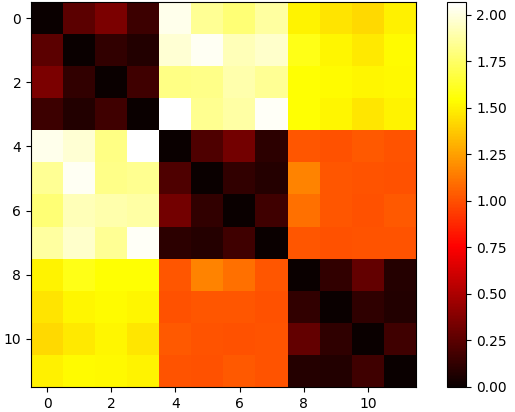
\includegraphics[width=0.7\linewidth]{figures/syntetic_data/distance_matrix/SO3.png}
    \caption[Classification using reparameterization of curves in \(\mathrm{SO}(3)\)]{Heat map of the distance matrix for twelve synthetic \(\mathrm{SO}(3)\) curves, denoted \(c_i^j\), where \(i \in \{1, 2, 3\}\) indicates the shape and \(j \in \{1, 2, 3, \text{eq}\}\) represents the parameterization. The color intensity reflects the shape space distance, with lower distances indicating similarity in shape and higher distances signifying distinct shapes.}
    \label{fig:classification-SO3}
\end{figure}

\begin{figure}
    \centering
    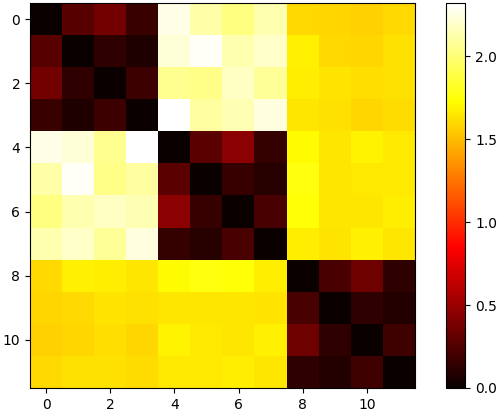
\includegraphics[width=0.7\linewidth]{figures/syntetic_data/distance_matrix/SE3.png}
    \caption[Classification using reparameterization of curves in \(\mathrm{SE}(3)\)]{Heat map of the distance matrix for twelve synthetic \(\mathrm{SE}(3)\) curves, denoted \(c_i^j\), where \(i \in \{1, 2, 3\}\) indicates the shape and \(j \in \{1, 2, 3, \text{eq}\}\) represents the parameterization. The color intensity reflects the shape space distance, with lower distances indicating similarity in shape and higher distances signifying distinct shapes.}
    \label{fig:classification-SE3}
\end{figure}

\begin{figure}
    \centering
    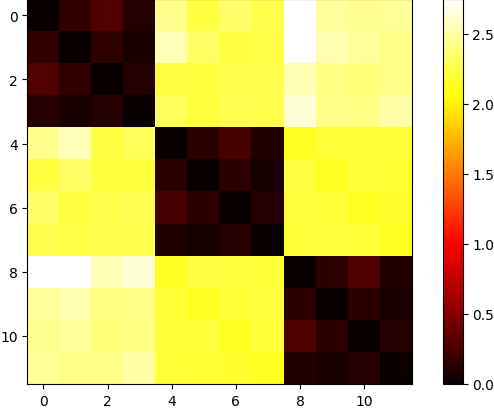
\includegraphics[width=0.7\linewidth]{figures/syntetic_data/distance_matrix/SO3_3.png}
    \caption[Classification using reparameterization of curves in \(\mathrm{SO}(3)^3\)]{Heat map of the distance matrix for twelve synthetic \(\mathrm{SO}(3)^3\) curves, denoted \(c_{(i,i+1,i+2)}^j\), where \(i \in \{1, 4, 7\}\) indicates the shape and \(j \in \{1, 2, 3, \text{eq}\}\) represents the parameterization. The color intensity reflects the shape space distance, with lower distances indicating similarity in shape and higher distances signifying distinct shapes.}
    \label{fig:classification-SO3-3}
\end{figure}

\begin{figure}
    \centering
    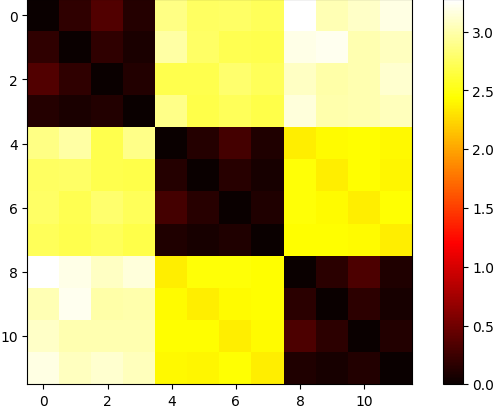
\includegraphics[width=0.7\linewidth]{figures/syntetic_data/distance_matrix/SE3_3.png}
    \caption[Classification using reparameterization of curves in \(\mathrm{SE}(3)^3\)]{Heat map of the distance matrix for twelve synthetic \(\mathrm{SE}(3)^3\) curves, denoted \(c_{(i,i+1,i+2)}^j\), where \(i \in \{1, 4, 7\}\) indicates the shape and \(j \in \{1, 2, 3, \text{eq}\}\) represents the parameterization. The color intensity reflects the shape space distance, with lower distances indicating similarity in shape and higher distances signifying distinct shapes.}
    \label{fig:classification-SE3-3}
\end{figure}

The classification outcomes for each dataset type \(\mathrm{SO}(3)\), \(\mathrm{SE}(3)\), \(\mathrm{SO}(3)^3\), and \(\mathrm{SE}(3)^3\) are depicted in Figures \ref{fig:classification-SO3}, \ref{fig:classification-SE3}, \ref{fig:classification-SO3-3}, and \ref{fig:classification-SE3-3}, respectively. These results highlight the efficacy of our methodology in distinguishing between curve shapes through reparameterization, demonstrating the robustness and utility of the proposed approach.

Notably, the classification is more precise for curves in \(\mathrm{SO}(3)^3\) and \(\mathrm{SE}(3)^3\). In these cases, the distances between curves of the same shape are significantly closer, while distances between curves of different shapes are more pronounced compared to those in \(\mathrm{SO}(3)\) and \(\mathrm{SE}(3)\). This suggests that our reparameterization framework is particularly effective in higher-dimensional settings, where it can better capture and distinguish subtle geometric differences.

\FloatBarrier
\subsubsection{Reduced Search Area}
\label{subsubsec:reduced-search-area}

In practical applications, exhaustive domain searches can be computationally demanding, as outlined in Subsection \ref{subsec:neighborhood-search-strategy}. This becomes impractical for large datasets or higher-dimensional spaces. To address this, we evaluate the impact of varying search depths on performance while maintaining a constant sample count. Our goal is to balance computational efficiency and accuracy by optimizing the search depth.

Figures \ref{fig:depth-error-single} and \ref{fig:depth-error-cartesian}, shows that the error decreases with increasing search depth across curves in \(\mathrm{SO}(3)\), \(\mathrm{SE}(3)\), \(\mathrm{SO}(3)^3\), and \(\mathrm{SE}(3)^3\). Initially, the error reduction is rapid, but it levels off as depth increases, with minimal differences observed between depths 4 and 10. This suggests diminishing returns in error reduction beyond a certain depth, which appears to be around search depth 4 for this dataset.

Figure \ref{fig:depth-error-time} illustrates the computation time required for these calculations. As expected, computation time increases significantly with greater search depth, though the growth is not strictly quadratic due to various operational efficiencies and the moderate scale of \(n\). These results highlight the need for an optimal search depth to balance accuracy and computational cost.

Based on these observations, we find that a search depth of 4 significantly reduces computation time while maintaining an acceptable error rate. This depth provides a practical balance between computational efficiency and accuracy, making it suitable for our reparameterization framework in both lower and higher-dimensional spaces. However, these findings are specific to the current dataset and may vary with different datasets.

\begin{figure}
    \centering
    \begin{subfigure}[c]{\textwidth}
        \begin{tikzpicture}
            \begin{axis}[
                width=0.8\textwidth,
                height=0.5\textwidth,
                ytick={0,1,2},
                xlabel={Search Depth},
                ylabel={\(d_{\mathcal{S}_*}\left(c^j, c^{\text{eq}}\right)\)},
                legend style={at={(1.05,0.5)}, anchor=west},
                grid=major,
            ]
            \addplot [thick, red, solid] table [x=depth, y=L2_distance, col sep=comma] {figures/syntetic_data/reparameterization_SO3/depth_error/g0_varphi0.csv};
            \addlegendentry{$c_1^1$}
    
            \addplot [thick, red, dashed] table [x=depth, y=L2_distance, col sep=comma] {figures/syntetic_data/reparameterization_SO3/depth_error/g0_varphi1.csv};
            \addlegendentry{$c_1^2$}
    
            \addplot [thick, red, dotted] table [x=depth, y=L2_distance, col sep=comma] {figures/syntetic_data/reparameterization_SO3/depth_error/g0_varphi2.csv};
            \addlegendentry{$c_1^3$}
    
            \addplot [thick, blue, solid] table [x=depth, y=L2_distance, col sep=comma] {figures/syntetic_data/reparameterization_SO3/depth_error/g1_varphi0.csv};
            \addlegendentry{$c_2^1$}
    
            \addplot [thick, blue, dashed] table [x=depth, y=L2_distance, col sep=comma] {figures/syntetic_data/reparameterization_SO3/depth_error/g1_varphi1.csv};
            \addlegendentry{$c_2^2$}
    
            \addplot [thick, blue, dotted] table [x=depth, y=L2_distance, col sep=comma] {figures/syntetic_data/reparameterization_SO3/depth_error/g1_varphi2.csv};
            \addlegendentry{$c_2^3$}
    
            \addplot [thick, green, solid] table [x=depth, y=L2_distance, col sep=comma] {figures/syntetic_data/reparameterization_SO3/depth_error/g2_varphi0.csv};
            \addlegendentry{$c_3^1$}
    
            \addplot [thick, green, dashed] table [x=depth, y=L2_distance, col sep=comma] {figures/syntetic_data/reparameterization_SO3/depth_error/g2_varphi1.csv};
            \addlegendentry{$c_3^2$}
    
            \addplot [thick, green, dotted] table [x=depth, y=L2_distance, col sep=comma] {figures/syntetic_data/reparameterization_SO3/depth_error/g2_varphi2.csv};
            \addlegendentry{$c_3^3$}
    
            \end{axis}
        \end{tikzpicture}
        \caption{}
    \end{subfigure}

    \centering
    \begin{subfigure}[c]{\textwidth}
        \begin{tikzpicture}
            \begin{axis}[
                width=0.8\textwidth,
                height=0.5\textwidth,
                xlabel={Search Depth},
                ylabel={\(d_{\mathcal{S}_*}\left(c^j, c^{\text{eq}}\right)\)},
                legend style={at={(1.05,0.5)}, anchor=west},
                grid=major,
            ]
            \addplot [thick, red, solid] table [x=depth, y=L2_distance, col sep=comma] {figures/syntetic_data/reparameterization_SE3/depth_error/g0_varphi0.csv};
            \addlegendentry{$c_1^1$}
    
            \addplot [thick, red, dashed] table [x=depth, y=L2_distance, col sep=comma] {figures/syntetic_data/reparameterization_SE3/depth_error/g0_varphi1.csv};
            \addlegendentry{$c_1^2$}
    
            \addplot [thick, red, dotted] table [x=depth, y=L2_distance, col sep=comma] {figures/syntetic_data/reparameterization_SE3/depth_error/g0_varphi2.csv};
            \addlegendentry{$c_1^3$}
    
            \addplot [thick, blue, solid] table [x=depth, y=L2_distance, col sep=comma] {figures/syntetic_data/reparameterization_SE3/depth_error/g1_varphi0.csv};
            \addlegendentry{$c_2^1$}
    
            \addplot [thick, blue, dashed] table [x=depth, y=L2_distance, col sep=comma] {figures/syntetic_data/reparameterization_SE3/depth_error/g1_varphi1.csv};
            \addlegendentry{$c_2^2$}
    
            \addplot [thick, blue, dotted] table [x=depth, y=L2_distance, col sep=comma] {figures/syntetic_data/reparameterization_SE3/depth_error/g1_varphi2.csv};
            \addlegendentry{$c_2^3$}
    
            \addplot [thick, green, solid] table [x=depth, y=L2_distance, col sep=comma] {figures/syntetic_data/reparameterization_SE3/depth_error/g2_varphi0.csv};
            \addlegendentry{$c_3^1$}
    
            \addplot [thick, green, dashed] table [x=depth, y=L2_distance, col sep=comma] {figures/syntetic_data/reparameterization_SE3/depth_error/g2_varphi1.csv};
            \addlegendentry{$c_3^2$}
    
            \addplot [thick, green, dotted] table [x=depth, y=L2_distance, col sep=comma] {figures/syntetic_data/reparameterization_SE3/depth_error/g2_varphi2.csv};
            \addlegendentry{$c_3^3$}
    
            \end{axis}
        \end{tikzpicture}
        \caption{}
    \end{subfigure}
    \caption[Convergence of Shape Distance with Increasing Search Depth in \(\mathrm{SO}(3)\) and \(\mathrm{SE}(3)\)]{Plot showing the convergence of shape distance \(d_{\mathcal{S}_*}\) (defined in Equation \eqref{eq:shape-space-metric-id}) between curve \(c_{i}^{\mathrm{eq}}\) and its reparameterization \(c_{i}^{j}\) for \(j \in \{1, 2, 3\}\) and \(i \in \{1, 2, 3\}\) within group \(G\) as search depth increases: (a) \(G = \mathrm{SO}(3)\), (b) \(G = \mathrm{SE}(3)\).}
    \label{fig:depth-error-single}
\end{figure}

\begin{figure}
    \centering
    \begin{subfigure}[c]{\textwidth}
        \begin{tikzpicture}
            \begin{axis}[
                width=0.8\textwidth,
                height=0.5\textwidth,
                xlabel={Search Depth},
                ylabel={\(d_{\mathcal{S}_*}\left(c^j, c^{\text{eq}}\right)\)},
                legend style={at={(1.05,0.5)}, anchor=west},
                grid=major,
            ]
            \addplot [thick, red, solid] table [x=depth, y=L2_distance, col sep=comma] {figures/syntetic_data/reparameterization_SO3_3/depth_error/g0_varphi0.csv};
            \addlegendentry{$c_{(1,2,3)}^1$}
    
            \addplot [thick, red, dashed] table [x=depth, y=L2_distance, col sep=comma] {figures/syntetic_data/reparameterization_SO3_3/depth_error/g0_varphi1.csv};
            \addlegendentry{$c_{(1,2,3)}^2$}
    
            \addplot [thick, red, dotted] table [x=depth, y=L2_distance, col sep=comma] {figures/syntetic_data/reparameterization_SO3_3/depth_error/g0_varphi2.csv};
            \addlegendentry{$c_{(1,2,3)}^3$}

            \addplot [thick, blue, solid] table [x=depth, y=L2_distance, col sep=comma] {figures/syntetic_data/reparameterization_SO3_3/depth_error/g1_varphi0.csv};
            \addlegendentry{$c_{(4,5,6)}^1$}
    
            \addplot [thick, blue, dashed] table [x=depth, y=L2_distance, col sep=comma] {figures/syntetic_data/reparameterization_SO3_3/depth_error/g1_varphi1.csv};
            \addlegendentry{$c_{(4,5,6)}^2$}
    
            \addplot [thick, blue, dotted] table [x=depth, y=L2_distance, col sep=comma] {figures/syntetic_data/reparameterization_SO3_3/depth_error/g1_varphi2.csv};
            \addlegendentry{$c_{(4,5,6)}^3$}
    
            \addplot [thick, green, solid] table [x=depth, y=L2_distance, col sep=comma] {figures/syntetic_data/reparameterization_SO3_3/depth_error/g2_varphi0.csv};
            \addlegendentry{$c_{(7,8,9)}^1$}
    
            \addplot [thick, green, dashed] table [x=depth, y=L2_distance, col sep=comma] {figures/syntetic_data/reparameterization_SO3_3/depth_error/g2_varphi1.csv};
            \addlegendentry{$c_{(7,8,9)}^2$}
    
            \addplot [thick, green, dotted] table [x=depth, y=L2_distance, col sep=comma] {figures/syntetic_data/reparameterization_SO3_3/depth_error/g2_varphi2.csv};
            \addlegendentry{$c_{(7,8,9)}^3$}
    
            \end{axis}
        \end{tikzpicture}
        \caption{}
    \end{subfigure}

    \centering
    \begin{subfigure}[c]{\textwidth}
        \begin{tikzpicture}
            \begin{axis}[
                width=0.8\textwidth,
                height=0.5\textwidth,
                xlabel={Search Depth},
                ylabel={\(d_{\mathcal{S}_*}\left(c^j, c^{\text{eq}}\right)\)},
                legend style={at={(1.05,0.5)}, anchor=west},
                grid=major,
            ]
            \addplot [thick, red, solid] table [x=depth, y=L2_distance, col sep=comma] {figures/syntetic_data/reparameterization_SE3_3/depth_error/g0_varphi0.csv};
            \addlegendentry{$c_{(1,2,3)}^1$}

            \addplot [thick, red, dashed] table [x=depth, y=L2_distance, col sep=comma] {figures/syntetic_data/reparameterization_SE3_3/depth_error/g0_varphi1.csv};
            \addlegendentry{$c_{(1,2,3)}^2$}
    
            \addplot [thick, red, dotted] table [x=depth, y=L2_distance, col sep=comma] {figures/syntetic_data/reparameterization_SE3_3/depth_error/g0_varphi2.csv};
            \addlegendentry{$c_{(1,2,3)}^3$}

            \addplot [thick, blue, solid] table [x=depth, y=L2_distance, col sep=comma] {figures/syntetic_data/reparameterization_SE3_3/depth_error/g1_varphi0.csv};
            \addlegendentry{$c_{(4,5,6)}^1$}
    
            \addplot [thick, blue, dashed] table [x=depth, y=L2_distance, col sep=comma] {figures/syntetic_data/reparameterization_SE3_3/depth_error/g1_varphi1.csv};
            \addlegendentry{$c_{(4,5,6)}^2$}
    
            \addplot [thick, blue, dotted] table [x=depth, y=L2_distance, col sep=comma] {figures/syntetic_data/reparameterization_SE3_3/depth_error/g1_varphi2.csv};
            \addlegendentry{$c_{(4,5,6)}^3$}
    
            \addplot [thick, green, solid] table [x=depth, y=L2_distance, col sep=comma] {figures/syntetic_data/reparameterization_SE3_3/depth_error/g2_varphi0.csv};
            \addlegendentry{$c_{(7,8,9)}^1$}
    
            \addplot [thick, green, dashed] table [x=depth, y=L2_distance, col sep=comma] {figures/syntetic_data/reparameterization_SE3_3/depth_error/g2_varphi1.csv};
            \addlegendentry{$c_{(7,8,9)}^2$}
    
            \addplot [thick, green, dotted] table [x=depth, y=L2_distance, col sep=comma] {figures/syntetic_data/reparameterization_SE3_3/depth_error/g2_varphi2.csv};
            \addlegendentry{$c_{(7,8,9)}^3$}
    
            \end{axis}
        \end{tikzpicture}  
        \caption{}
    \end{subfigure}
    \caption[Convergence of Shape Distance with Increasing Search Depth in \(\mathrm{SO}(3)^3\) and \(\mathrm{SE}(3)^3\)]{Plot showing the convergence of shape distance \(d_{\mathcal{S}_*}\) (defined in Equation \eqref{eq:shape-space-metric-id}) between curve \(c_{i,i+1,i+2}^{\text{eq}}\) and its reparameterization \(c_{i,i+1,i+2}^{j}\) for \(j \in \{1,2,3\}\) and \(i \in \{1, 4, 7\}\) within group \(G\) as search depth increases: (a) \(G = \mathrm{SO}(3)^3\), (b) \(G = \mathrm{SE}(3)^3\).}
    \label{fig:depth-error-cartesian}
\end{figure}

\begin{figure}
    \centering
    \begin{tikzpicture}
        \begin{axis}[
            width=0.7\textwidth,
            height=0.5\textwidth,
            xlabel={Search Depth},
            ylabel={Mean Time (seconds)},
            legend style={at={(1.05,0.5)}, anchor=west},
            grid=major,
        ]
        \addplot [thick, red, solid] table [x=depth, y=mean_time, col sep=comma] {figures/syntetic_data/reparameterization_SO3/depth_error/mean_time.csv};
        \addlegendentry{\(c \in \mathrm{SO}(3)\)}

        \addplot [thick, blue, solid] table [x=depth, y=mean_time, col sep=comma] {figures/syntetic_data/reparameterization_SE3/depth_error/mean_time.csv};
        \addlegendentry{\(c \in \mathrm{SE}(3)\)}

        \addplot [thick, red, dotted] table [x=depth, y=mean_time, col sep=comma] {figures/syntetic_data/reparameterization_SO3_3/depth_error/mean_time.csv};
        \addlegendentry{\(c \in \mathrm{SO}(3)^3\)}

        \addplot [thick, blue, dotted] table [x=depth, y=mean_time, col sep=comma] {figures/syntetic_data/reparameterization_SE3_3/depth_error/mean_time.csv};
        \addlegendentry{\(c \in \mathrm{SE}(3)^3\)}

        \end{axis}
    \end{tikzpicture}    
    \caption[Computation Time for Dynamic Programming at Various Search Depths]{Mean computation time required for curve reparameterization across varying search depths (100 time steps). The mean values are calculated based on the time taken to compute errors for each curve, considering different reparameterizations and search depths. The associated errors are shown in the Figures \ref{fig:depth-error-single} and \ref{fig:depth-error-cartesian}.}
    \label{fig:depth-error-time}
\end{figure}

\subsubsection{Perturbation Analysis}
\label{subsubsec:perturbation-analysis}

In this part, we examine the effects of perturbations on a curve by analyzing both the pseudometric \(d_{\mathcal{P}_*}\) and the shape distance \(d_{\mathcal{S}_*}\) between the equidistant parameterized curve \(c^{\text{eq}}\) and its perturbed counterpart \(c^\epsilon\). The perturbed curves \(c^\epsilon\) are generated by solving the differential equation \(g' = g \hat{u}(t)\), where \(u(t) = \omega_i(t)\) or \(u(t) = \xi_i(t)\), with \(t\) perturbed by a normal distribution.
Previously In Section \ref{subsubsec:perturbation-analysis}, we found that the order of the distance between the original and reparameterized curves was bounded from below by \(1/2\). Here, we further analyze perturbations on curves in \(\mathrm{SO}(3)\) and \(\mathrm{SE}(3)\) using \(d_{\mathcal{P}_*}\), and employ dynamic programming with depth 10 to examine the impact on \(d_{\mathcal{S}_*}\). Figure \ref{fig:perturbation-analysis-dp} illustrates \(d_{\mathcal{P}_*}\), and Figure \ref{fig:perturbation-analysis-ds} shows \(d_{\mathcal{S}_*}\) for synthetic curves in \(\mathrm{SO}(3)\) and \(\mathrm{SE}(3)\) with varying perturbation magnitudes \(\epsilon\). Solid lines represent rotational components \(\omega_1, \omega_2, \omega_3\), and dashed lines represent combined rotational and translational components \(\xi_1, \xi_2, \xi_3\).

\begin{figure}
    \centering
    \begin{tikzpicture}
        \begin{loglogaxis}[
            width=0.95\textwidth,
            height=0.4\textwidth,
            xlabel={\(\epsilon\)},
            ylabel={\(d_{\mathcal{P}_*}(c^{\epsilon}, c^{\text{eq}})\)},
            legend style={font=\small, at={(1.05,0.5)}, anchor=west},
            grid=major,
            legend pos=north west,
        ]
        
        \addplot [thick, red, solid] table [x=perturbation, y=c1, col sep=comma] {figures/syntetic_data/perturbation-analysis/SO3.csv};
        \addlegendentry{\(\omega_1\)}

        \addplot [thick, blue, solid] table [x=perturbation, y=c2, col sep=comma] {figures/syntetic_data/perturbation-analysis/SO3.csv};
        \addlegendentry{\(\omega_2\)}

        \addplot [thick, green, solid] table [x=perturbation, y=c3, col sep=comma] {figures/syntetic_data/perturbation-analysis/SO3.csv};
        \addlegendentry{\(\omega_3\)}

        \addplot [thick, red, dashed] table [x=perturbation, y=c1, col sep=comma] {figures/syntetic_data/perturbation-analysis/SE3.csv};
        \addlegendentry{\(\xi_1\)}

        \addplot [thick, blue, dashed] table [x=perturbation, y=c2, col sep=comma] {figures/syntetic_data/perturbation-analysis/SE3.csv};
        \addlegendentry{\(\xi_2\)}

        \addplot [thick, green, dashed] table [x=perturbation, y=c3, col sep=comma] {figures/syntetic_data/perturbation-analysis/SE3.csv};
        \addlegendentry{\(\xi_3\)}

        \logLogSlopeTriangle{0.7}{0.3}{0.2}{1}{black, dashed}
        
        \end{loglogaxis}
    \end{tikzpicture}
    \caption[Perturbation Analysis of Curves Using \(d_{\mathcal{P}_*}\)]{This figure illustrates the perturbation analysis of synthetic curves within the groups \(\mathrm{SO}(3)\) and \(\mathrm{SE}(3)\). Displayed is the pseudometric \(d_{\mathcal{P}_*}\) between the baseline curve \(c^\text{eq}\) and its perturbed form \(c^\epsilon\), under perturbations of varying magnitudes \(\epsilon\). The dashed black triangle marks the convergence of order 1.}
    \label{fig:perturbation-analysis-dp}
\end{figure}

\begin{figure}
    \centering
    \begin{tikzpicture}
        \begin{loglogaxis}[
            width=0.95\textwidth,
            height=0.4\textwidth,
            xlabel={\(\epsilon\)},
            ylabel={\(d_{\mathcal{S}_*}(c^{\epsilon}, c^{\text{eq}})\)},
            legend style={font=\small, at={(1.05,0.5)}, anchor=west},
            grid=major,
            legend pos=north west,
        ]
        
        \addplot [thick, red, solid] table [x=perturbation, y=c1, col sep=comma] {figures/syntetic_data/perturbation-analysis/reparameterized-SO3.csv};
        \addlegendentry{\(\omega_1\)}

        \addplot [thick, blue, solid] table [x=perturbation, y=c2, col sep=comma] {figures/syntetic_data/perturbation-analysis/reparameterized-SO3.csv};
        \addlegendentry{\(\omega_2\)}

        \addplot [thick, green, solid] table [x=perturbation, y=c3, col sep=comma] {figures/syntetic_data/perturbation-analysis/reparameterized-SO3.csv};
        \addlegendentry{\(\omega_3\)}

        \addplot [thick, red, dashed] table [x=perturbation, y=c1, col sep=comma] {figures/syntetic_data/perturbation-analysis/reparameterized-SE3.csv};
        \addlegendentry{\(\xi_1\)}

        \addplot [thick, blue, dashed] table [x=perturbation, y=c2, col sep=comma] {figures/syntetic_data/perturbation-analysis/reparameterized-SE3.csv};
        \addlegendentry{\(\xi_2\)}

        \addplot [thick, green, dashed] table [x=perturbation, y=c3, col sep=comma] {figures/syntetic_data/perturbation-analysis/reparameterized-SE3.csv};
        \addlegendentry{\(\xi_3\)}

        \logLogSlopeTriangle{0.7}{0.3}{0.2}{1}{black, dashed}
        
        \end{loglogaxis}
    \end{tikzpicture}
    \caption[Perturbation Analysis of Curves Using \(d_{\mathcal{S}_*}\)]{This figure presents a reparameterized perturbation analysis for synthetic curves in \(\mathrm{SO}(3)\) and \(\mathrm{SE}(3)\), focusing on the shape distance \(d_{\mathcal{S}_*}\). It shows how \(d_{\mathcal{S}_*}\) varies between the curve \(c^{\text{eq}}\) and its perturbed version \(c^\epsilon\) under different perturbation magnitudes \(\epsilon\). The convergence rate of order 1 is indicated by a dashed black triangle. Reparameterization was executed using dynamic programming with a search depth of 10.}
    \label{fig:perturbation-analysis-ds}
\end{figure}

From Figure \ref{fig:perturbation-analysis-dp}, the convergence rate of order 1 suggests our previous analysis may have been too pessimistic. In Figure \ref{fig:perturbation-analysis-ds}, \(d_{\mathcal{S}_*}\) is lower than \(d_{\mathcal{P}_*}\) for large perturbations, but they converge as perturbation decreases, indicating \(d_{\mathcal{S}_*}\) does not fully mitigate perturbations. To improve these results, a semidiscrete method as discussed in \cite{woienSemiDiscretizedMethodOptimal2019} may be employed.









\FloatBarrier
\section[Optimal Curve Reparameterization through Geodesic Interpolation]{Optimal Curve Reparameterization through \\ Geodesic Interpolation}
\label{sec:optimal-curve-reparameterization}

This section presents an optimal reparameterization technique for curve alignment within Lie groups, particularly \(\mathrm{SO}(3)\) and \(\mathrm{SE}(3)\). Unlike the dynamic programming approach in Section \ref{sec:dynamic-programming}, this method provides a continuous framework for curve comparison over the domain \([0,1]\) without a fixed set of nodes. As it does not use the SRVT framework (discussed in \ref{subsec:srvt}), this approach may result in very small geodesic distances for curves of different shapes. It is mainly applied to align curves with assumed identical shapes.

\subsection{Overview of methodology}
\label{subsec:methodology-overview-geodesic-interpolation}

The goal is to reparameterize a discrete curve \(g\) in a Lie group \(G\) to minimize the shape distance to another curve \(h\). This is achieved by identifying a diffeomorphism \(\varphi \in \mathrm{Diff}^+([0,1])\) that transforms \(g\) into \(g_\varphi(t) = g(\varphi(t))\) for \(t \in [0,1]\), aligning it with \(h\) at specific points. Geodesic interpolation facilitates detailed comparisons throughout \([0,1]\), not limited to discrete points.

The alignment's objective function is formulated as:
\begin{equation}
    C(s_k^\varphi) = \sum_{k=0}^N \| \log(g(s_k^\varphi)^{-1} h(s_k)) \|_F^2,
    \label{eq:cost-function-geodesic-interpolation}
\end{equation}
where \(s_k\) are equidistant nodes along \(h\) and \(s_k^\varphi = \varphi(s_k)\) are the transformed nodes of \(g\).

For multi-component curves \(g_i\) and \(h_i\), the function expands to:
\begin{equation}
    C(s_k^\varphi) = \sum_{i=1}^n \sum_{k=0}^N \| \log(g_i(s_k^\varphi)^{-1} h_i(s_k)) \|_F^2,
    \label{eq:cost-function-geodesic-interpolation-cartesian}
\end{equation}
where \(g_i\) and \(h_i\) are the i-th components of the curves \(g\) and \(h\).

Minimizing \(C(s_k^\varphi)\) can be done in several ways, but is here performed using Sequential Least Squares Quadratic Programming (SLSQP) via \texttt{scipy.optimize} \cite{virtanenSciPyFundamentalAlgorithms2020}, ensuring an increasing \(\varphi\) and mitigating local minima with multiple randomized initializations.

\subsection{Numerical Analysis}
\label{subsec:geodesic-interpolation-analysis}

This subsection evaluates the performance of our reparameterization framework on synthetic data. We first reparameterize synthetic curves of the same shape, and then explore its application for classification.

\subsubsection{Reparameterization of Curves}
\label{subsubsec:reparameterization-curves}

For this analysis, we use synthetic data generated as described in \ref{subsec:synthetic-data-generation}. We reparameterize equidistant curves \(c_i^\text{eq}\) and \(c_{i,i+1,i+2}^\text{eq}\) to match parameterized curves \(c_i^j\) and \(c_{i,i+1,i+2}^j\), respectively, as in the dynamic programming approach described in \ref{subsec:reparameterization-curves}. The quality of reparameterization is assessed by comparing the resulting reparameterizations \(\hat{\varphi}_j^i\) with the original parameterizations \(\varphi_j\). 

\begin{figure}[!ht]
    \begin{tikzpicture}
        \begin{axis}[
            width=0.85\textwidth,
            height=0.55\textwidth,
            xlabel={\( x \)},
            ylabel={\( \varphi(x) \)},
            grid=major,
            grid style={dashed,gray!30},
            legend style={at={(1.05,0.5)}, anchor=west},
            line width=1pt,
            xmin=0, xmax=1,
            ymin=0, ymax=1
        ]
        \addplot [thin, red, solid] table [x=x, y=varphi_1, col sep=comma] {figures/syntetic_data/parameterization/varphi_1.csv};
        \addlegendentry{\( \varphi_1\)}

        \addplot [thin, blue, solid] table [x=x, y=varphi_2, col sep=comma] {figures/syntetic_data/parameterization/varphi_2.csv};
        \addlegendentry{\( \varphi_2\)}

        \addplot [thin, green, solid] table [x=x, y=varphi_3, col sep=comma] {figures/syntetic_data/parameterization/varphi_3.csv};
        \addlegendentry{\( \varphi_3\)}


        \addplot [red, dashed] table [x=x, y=g0, col sep=comma] {figures/syntetic_data/reparameterization_SO3_SLERP/df_varphi_1.csv};
        \addlegendentry{\( \hat \varphi_{1}^{1}\)}

        \addplot [red, dotted] table [x=x, y=g1, col sep=comma] {figures/syntetic_data/reparameterization_SO3_SLERP/df_varphi_1.csv};
        \addlegendentry{\( \hat \varphi_{1}^{2}\)}

        \addplot [red, dashdotted] table [x=x, y=g2, col sep=comma] {figures/syntetic_data/reparameterization_SO3_SLERP/df_varphi_1.csv};
        \addlegendentry{\( \hat \varphi_{1}^{3}\)}

        \addplot [blue, dashed] table [x=x, y=g0, col sep=comma] {figures/syntetic_data/reparameterization_SO3_SLERP/df_varphi_2.csv};
        \addlegendentry{\( \hat \varphi_{2}^{1}\)}

        \addplot [blue, dotted] table [x=x, y=g1, col sep=comma] {figures/syntetic_data/reparameterization_SO3_SLERP/df_varphi_2.csv};
        \addlegendentry{\( \hat \varphi_{2}^{2}\)}

        \addplot [blue, dashdotted] table [x=x, y=g2, col sep=comma] {figures/syntetic_data/reparameterization_SO3_SLERP/df_varphi_2.csv};
        \addlegendentry{\( \hat \varphi_{2}^{3}\)}

        \addplot [green, dashed] table [x=x, y=g0, col sep=comma] {figures/syntetic_data/reparameterization_SO3_SLERP/df_varphi_3.csv};
        \addlegendentry{\( \hat \varphi_{3}^{1}\)}

        \addplot [green, dotted] table [x=x, y=g1, col sep=comma] {figures/syntetic_data/reparameterization_SO3_SLERP/df_varphi_3.csv};
        \addlegendentry{\( \hat \varphi_{3}^{2}\)}

        \addplot [green, dashdotted] table [x=x, y=g2, col sep=comma] {figures/syntetic_data/reparameterization_SO3_SLERP/df_varphi_3.csv};
        \addlegendentry{\( \hat \varphi_{3}^{3}\)}

        \end{axis}
    \end{tikzpicture}    
    \caption[Reparameterization of Curves in \(\mathrm{SO}(3)\)]{Comparison of reparameterization results for \(\mathrm{SO}(3)\) data, showing \(\hat{\varphi}_j^{i}\) obtained from our framework versus the analytical \(\varphi_j\). Here, \(j \in \{1, 2, 3\}\) denotes the mappings, and \(i \in \{1, 2, 3\}\) indicates the shapes. Colors represent different mappings, while line styles distinguish the shapes, illustrating the accuracy of the fit.}
    \label{fig:reparameterization-SO3-SLERP}
\end{figure}

\begin{figure}[!ht]
    \begin{tikzpicture}
        \begin{axis}[
            width=0.8\textwidth,
            height=0.55\textwidth,
            xlabel={\( x \)},
            ylabel={\( \varphi(x) \)},
            grid=major,
            grid style={dashed,gray!30},
            legend style={at={(1.05,0.5)}, anchor=west},
            line width=1pt,
            xmin=0, xmax=1,
            ymin=0, ymax=1
        ]
        \addplot [thin, red, solid] table [x=x, y=varphi_1, col sep=comma] {figures/syntetic_data/parameterization/varphi_1.csv};
        \addlegendentry{\( \varphi_1\)}

        \addplot [thin, blue, solid] table [x=x, y=varphi_2, col sep=comma] {figures/syntetic_data/parameterization/varphi_2.csv};
        \addlegendentry{\( \varphi_2\)}

        \addplot [thin, green, solid] table [x=x, y=varphi_3, col sep=comma] {figures/syntetic_data/parameterization/varphi_3.csv};
        \addlegendentry{\( \varphi_3\)}


        \addplot [red, dashed] table [x=x, y=g0, col sep=comma] {figures/syntetic_data/reparameterization_SO3_3_SLERP/df_varphi_1.csv};
        \addlegendentry{\( \hat \varphi_{1}^{(1,2,3)}\)}

        \addplot [red, dotted] table [x=x, y=g1, col sep=comma] {figures/syntetic_data/reparameterization_SO3_3_SLERP/df_varphi_1.csv};
        \addlegendentry{\( \hat \varphi_{1}^{(4,5,6)}\)}

        \addplot [red, dashdotted] table [x=x, y=g2, col sep=comma] {figures/syntetic_data/reparameterization_SO3_3_SLERP/df_varphi_1.csv};
        \addlegendentry{\( \hat \varphi_{1}^{(7,8,9)}\)}

        \addplot [blue, dashed] table [x=x, y=g0, col sep=comma] {figures/syntetic_data/reparameterization_SO3_3_SLERP/df_varphi_2.csv};
        \addlegendentry{\( \hat \varphi_{2}^{(1,2,3)}\)}

        \addplot [blue, dotted] table [x=x, y=g1, col sep=comma] {figures/syntetic_data/reparameterization_SO3_3_SLERP/df_varphi_2.csv};
        \addlegendentry{\( \hat \varphi_{2}^{(4,5,6)}\)}

        \addplot [blue, dashdotted] table [x=x, y=g2, col sep=comma] {figures/syntetic_data/reparameterization_SO3_3_SLERP/df_varphi_2.csv};
        \addlegendentry{\( \hat \varphi_{2}^{(7,8,9)}\)}

        \addplot [green, dashed] table [x=x, y=g0, col sep=comma] {figures/syntetic_data/reparameterization_SO3_3_SLERP/df_varphi_3.csv};
        \addlegendentry{\( \hat \varphi_{3}^{(1,2,3)}\)}

        \addplot [green, dotted] table [x=x, y=g1, col sep=comma] {figures/syntetic_data/reparameterization_SO3_3_SLERP/df_varphi_3.csv};
        \addlegendentry{\( \hat \varphi_{3}^{(4,5,6)}\)}

        \addplot [green, dashdotted] table [x=x, y=g2, col sep=comma] {figures/syntetic_data/reparameterization_SO3_3_SLERP/df_varphi_3.csv};
        \addlegendentry{\( \hat \varphi_{3}^{(7,8,9)}\)}
        \end{axis}
    \end{tikzpicture}    
    \caption[Reparameterization of Curves in \(\mathrm{SO}(3)^3\)]{Comparison of reparameterization results for \(\mathrm{SO}(3)^3\) data, showing \(\hat{\varphi}_j^{i,i+1,i+2}\) obtained from our framework versus the analytical \(\varphi_j\). Here, \(j \in \{1, 2, 3\}\) denotes the mappings, and \(i \in \{1, 4, 7\}\) indicates the shapes. Colors represent different mappings, while line styles distinguish the shapes, illustrating the accuracy of the fit.}
    \label{fig:reparameterization-SO3-3-SLERP}
\end{figure}

\begin{figure}[!ht]
    \begin{tikzpicture}
        \begin{axis}[
            width=0.85\textwidth,
            height=0.55\textwidth,
            xlabel={\( x \)},
            ylabel={\( \varphi(x) \)},
            grid=major,
            grid style={dashed,gray!30},
            legend style={at={(1.05,0.5)}, anchor=west},
            line width=1pt,
            xmin=0, xmax=1,
            ymin=0, ymax=1
        ]
        \addplot [thin, red, solid] table [x=x, y=varphi_1, col sep=comma] {figures/syntetic_data/parameterization/varphi_1.csv};
        \addlegendentry{\( \varphi_1\)}

        \addplot [thin, blue, solid] table [x=x, y=varphi_2, col sep=comma] {figures/syntetic_data/parameterization/varphi_2.csv};
        \addlegendentry{\( \varphi_2\)}

        \addplot [thin, green, solid] table [x=x, y=varphi_3, col sep=comma] {figures/syntetic_data/parameterization/varphi_3.csv};
        \addlegendentry{\( \varphi_3\)}

        \addplot [red, dashed] table [x=x, y=g0, col sep=comma] {figures/syntetic_data/reparameterization_SE3_SLERP/df_varphi_1.csv};
        \addlegendentry{\( \hat \varphi_{1}^1\)}

        \addplot [red, dotted] table [x=x, y=g1, col sep=comma] {figures/syntetic_data/reparameterization_SE3_SLERP/df_varphi_1.csv};
        \addlegendentry{\( \hat \varphi_{1}^2\)}

        \addplot [red, dashdotted] table [x=x, y=g2, col sep=comma] {figures/syntetic_data/reparameterization_SE3_SLERP/df_varphi_1.csv};
        \addlegendentry{\( \hat \varphi_{1}^3\)}

        \addplot [blue, dashed] table [x=x, y=g0, col sep=comma] {figures/syntetic_data/reparameterization_SE3_SLERP/df_varphi_2.csv};
        \addlegendentry{\( \hat \varphi_{2}^1\)}

        \addplot [blue, dotted] table [x=x, y=g1, col sep=comma] {figures/syntetic_data/reparameterization_SE3_SLERP/df_varphi_2.csv};
        \addlegendentry{\( \hat \varphi_{2}^2\)}

        \addplot [blue, dashdotted] table [x=x, y=g2, col sep=comma] {figures/syntetic_data/reparameterization_SE3_SLERP/df_varphi_2.csv};
        \addlegendentry{\( \hat \varphi_{2}^3\)}

        \addplot [green, dashed] table [x=x, y=g0, col sep=comma] {figures/syntetic_data/reparameterization_SE3_SLERP/df_varphi_3.csv};
        \addlegendentry{\( \hat \varphi_{3}^1\)}

        \addplot [green, dotted] table [x=x, y=g1, col sep=comma] {figures/syntetic_data/reparameterization_SE3_SLERP/df_varphi_3.csv};
        \addlegendentry{\( \hat \varphi_{3}^2\)}

        \addplot [green, dashdotted] table [x=x, y=g2, col sep=comma] {figures/syntetic_data/reparameterization_SE3_SLERP/df_varphi_3.csv};
        \addlegendentry{\( \hat \varphi_{3}^3\)}

        \end{axis}
    \end{tikzpicture}    
    \caption[Reparameterization of Curves in \(\mathrm{SE}(3)\)]{Comparison of reparameterization results for \(\mathrm{SE}(3)\) data, showing \(\hat{\varphi}_j^{i}\) obtained from our framework versus the analytical \(\varphi_j\). Here, \(j \in \{1, 2, 3\}\) denotes the mappings, and \(i \in \{1, 2, 3\}\) indicates the shapes. Colors represent different mappings, while line styles distinguish the shapes, illustrating the accuracy of the fit.}
    \label{fig:reparameterization-SE3-SLERP}
\end{figure}

\begin{figure}[!ht]
    \begin{tikzpicture}
        \begin{axis}[
            width=0.8\textwidth,
            height=0.55\textwidth,
            xlabel={\( x \)},
            ylabel={\( \varphi(x) \)},
            grid=major,
            grid style={dashed,gray!30},
            legend style={at={(1.05,0.5)}, anchor=west},
            line width=1pt,
            xmin=0, xmax=1,
            ymin=0, ymax=1
        ]
        \addplot [thin, red, solid] table [x=x, y=varphi_1, col sep=comma] {figures/syntetic_data/parameterization/varphi_1.csv};
        \addlegendentry{\( \varphi_1\)}

        \addplot [thin, blue, solid] table [x=x, y=varphi_2, col sep=comma] {figures/syntetic_data/parameterization/varphi_2.csv};
        \addlegendentry{\( \varphi_2\)}

        \addplot [thin, green, solid] table [x=x, y=varphi_3, col sep=comma] {figures/syntetic_data/parameterization/varphi_3.csv};
        \addlegendentry{\( \varphi_3\)}


        \addplot [red, dashed] table [x=x, y=g0, col sep=comma] {figures/syntetic_data/reparameterization_SE3_3_SLERP/df_varphi_1.csv};
        \addlegendentry{\( \hat \varphi_{1}^{(1,2,3)}\)}

        \addplot [red, dotted] table [x=x, y=g1, col sep=comma] {figures/syntetic_data/reparameterization_SE3_3_SLERP/df_varphi_1.csv};
        \addlegendentry{\( \hat \varphi_{1}^{(4,5,6)}\)}

        \addplot [red, dashdotted] table [x=x, y=g2, col sep=comma] {figures/syntetic_data/reparameterization_SE3_3_SLERP/df_varphi_1.csv};
        \addlegendentry{\( \hat \varphi_{1}^{(7,8,9)}\)}

        \addplot [blue, dashed] table [x=x, y=g0, col sep=comma] {figures/syntetic_data/reparameterization_SE3_3_SLERP/df_varphi_2.csv};
        \addlegendentry{\( \hat \varphi_{2}^{(1,2,3)}\)}

        \addplot [blue, dotted] table [x=x, y=g1, col sep=comma] {figures/syntetic_data/reparameterization_SE3_3_SLERP/df_varphi_2.csv};
        \addlegendentry{\( \hat \varphi_{2}^{(4,5,6)}\)}

        \addplot [blue, dashdotted] table [x=x, y=g2, col sep=comma] {figures/syntetic_data/reparameterization_SE3_3_SLERP/df_varphi_2.csv};
        \addlegendentry{\( \hat \varphi_{2}^{(7,8,9)}\)}

        \addplot [green, dashed] table [x=x, y=g0, col sep=comma] {figures/syntetic_data/reparameterization_SE3_3_SLERP/df_varphi_3.csv};
        \addlegendentry{\( \hat \varphi_{3}^{(1,2,3)}\)}

        \addplot [green, dotted] table [x=x, y=g1, col sep=comma] {figures/syntetic_data/reparameterization_SE3_3_SLERP/df_varphi_3.csv};
        \addlegendentry{\( \hat \varphi_{3}^{(4,5,6)}\)}

        \addplot [green, dashdotted] table [x=x, y=g2, col sep=comma] {figures/syntetic_data/reparameterization_SE3_3_SLERP/df_varphi_3.csv};
        \addlegendentry{\( \hat \varphi_{3}^{(7,8,9)}\)}

        \end{axis}
    \end{tikzpicture}    
    \caption[Reparameterization of Curves in \(\mathrm{SE}(3)^3\)]{Comparison of reparameterization results for \(\mathrm{SE}(3)^3\) data, showing \(\hat{\varphi}_j^{i,i+1,i+2}\) obtained from our framework versus the analytical \(\varphi_j\). Here, \(j \in \{1, 2, 3\}\) denotes the mappings, and \(i \in \{1, 4, 7\}\) indicates the shapes. Colors represent different mappings, while line styles distinguish the shapes, illustrating the accuracy of the fit.}
    \label{fig:reparameterization-SE3-3-SLERP}
\end{figure}

The effectiveness of these reparameterizations is visually demonstrated in Figures \ref{fig:reparameterization-SO3-SLERP}, \ref{fig:reparameterization-SO3-3-SLERP}, \ref{fig:reparameterization-SE3-SLERP}, and \ref{fig:reparameterization-SE3-3-SLERP}. These figures show alignment improvements, where true parameterizations are represented by solid lines, and reparameterization results by dashed, dotted, and dash-dotted lines. Colors indicate shapes, and line styles represent mappings.

The results show that the reparameterization framework aligns the curves well with the true parameterizations. The curves are closely matched, demonstrating the method's effectiveness. While some discrepancies are observed, especially in Figure \ref{fig:reparameterization-SO3-SLERP}, this may be due to local minima or insufficient runtime due to the method's computational expense, and should be further investigated.

\subsubsection{Classification of Curves}
\label{subsubsec:classification-curves}

We use the same synthetic data to classify curves based on their shapes. The classification is performed by computing the shape space distance between the curves using the cost functions \eqref{eq:cost-function-geodesic-interpolation} and \eqref{eq:cost-function-geodesic-interpolation-cartesian}. We store the cost between each pair of curves in a distance matrix. The distance matrix is visualized through heatmaps, where color intensity indicates the shape space distance between the curves, as shown in Figures \ref{fig:classification-SO3-interpolation} and \ref{fig:classification-SE3-interpolation}. We did not perform this classification on the curves in \(\mathrm{SE}(3)^3\) and \(\mathrm{SO}(3)^3\) due to the high computational expense and the method's unsuitability for comparing curves of different shapes.

\begin{figure}[!ht]
    \centering
    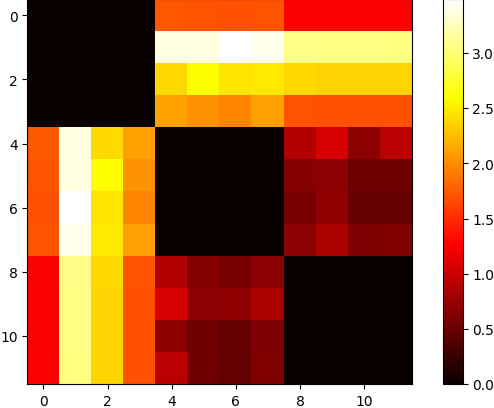
\includegraphics[width=0.6\linewidth]{figures/syntetic_data/distance_matrix/SO3_interpolation}
    \caption[Classification using interpolation to reparameterization of curves in \(\mathrm{SO}(3)\)]{Classification of synthetic \(\mathrm{SO}(3)\) curves across 100 timesteps, with geodesic interpolation to reparameterize, depicted as a distance matrix of twelve curves, denoted \(c_i^j\), where \(i = 1, 2, 3\) and \(j = 1, 2, 3, 4\). The color intensity within the matrix indicates the shape space distance.}
    \label{fig:classification-SO3-interpolation}
\end{figure}

\begin{figure}[!ht]
    \centering
    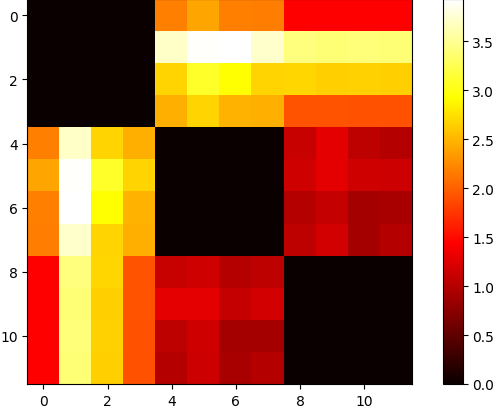
\includegraphics[width=0.6\linewidth]{figures/syntetic_data/distance_matrix/SE3_interpolation}
    \caption[Classification using interpolation to reparameterization of curves in \(\mathrm{SE}(3)\)]{Classification of synthetic \(\mathrm{SE}(3)\) curves across 100 timesteps, with geodesic interpolation to reparameterize, illustrated as a distance matrix of twelve curves, denoted \(c_i^j\), where \(i = 1, 2, 3\) and \(j = 1, 2, 3, 4\). The color intensity within the matrix indicates the shape space distance.}
    \label{fig:classification-SE3-interpolation}
\end{figure}

\FloatBarrier
As seen in the heatmaps, the classification is successful, with almost zero intra-class distances and high inter-class distances. This indicates that the curves are well separated in the shape space, and the classification is accurate. While these results are promising, we refrain from using this method for classifying motion capture data due to uncertainties about its robustness.

% \section{Summary}
\label{subsec:summary-reparam}
Summarize the key points discussed, reflect on the implications of optimal reparametrization, and suggest directions for future research.


\chapter{Signature Method}   
\label{ch:signature-method}

This chapter delves into the intricacies of the signature method, a robust tool for analyzing paths and curves. We explore its fundamental concepts, including tensor algebra and the definition of the signature along with its properties. Additionally, we investigate the logarithmic signature for path representation. The chapter culminates with numerical examples illustrating the method's application in shape analysis.

\section{Fundamentals of the Signature Method}
\label{sec:signature-fundamentals}

This section delves into the foundational aspects of the signature method, including tensor algebra, the definition of the signature, and its properties.

\subsection{Tensor Algebra and Its Dual Space}
\label{subsec:tensor-algebra}

Within the context of a finite-dimensional vector space \(V\) with dimension \(d\), the tensor algebra \(T(V)\) encompasses all tensor powers of \(V\):
\begin{equation}
    T(V) := \bigoplus_{n=0}^{\infty} V^{\otimes n} = \mathbb{R} \oplus V \oplus (V \otimes V) \oplus (V \otimes V \otimes V) \oplus \cdots,
\end{equation}
where \(V^{\otimes n}\) denotes the \(n\)-th tensor product of \(V\) and \(V^{\otimes 0} = \mathbb{R}\) \cite{chenAlgebrasIteratedPath1971}.

The dual space of the tensor algebra, denoted \(T((V)) := T(V)^*\) or \(T(V^*)\), represents the domain of formal power series in \(d\) non-commuting variables, represented by the set \(\{e_1, \ldots, e_d\}\) \cite{chenIntegrationPathsGeometric1957}.

In a \(d\)-dimensional vector space, tensor series are depicted as infinite vectors indexed by words from the alphabet \(\{1, \ldots, d\}\). Each word \(w = i_1 \cdots i_n\), with \(i_j\) drawn from \(\{1, \ldots, d\}\), corresponds to a fundamental element \(e_w = e_{i_1} \otimes \cdots \otimes e_{i_n}\) \cite{chevyrevPrimerSignatureMethod2016}. This conceptual framework serves as the cornerstone for defining iterated integrals of a path in \(\mathbb{R}^d\).

\subsection{Definition of the Signature}
\label{subsec:signature-definition}

For a smooth path \(x : [s, t] \to \mathbb{R}^d\) over \( [s, t] \subset [0, 1]\), the \(n\)-fold iterated integral for a word \(w = i_1 \cdots i_n\) is defined as:
\begin{equation}
\langle S(x)_{s,t}, e_w \rangle = \int_{s < u_n < \cdots < u_1 < t} dx_{u_1}^{i_1} \cdots dx_{u_n}^{i_n}.
\end{equation}
This provides geometric insights into the path \(x\) \cite{lyonsRoughPathsSignatures2014}.

The signature \(S(x)_{s,t}\) of \(x\) over \( [s, t] \) is represented by the tensor series:
\begin{equation}
S(x)_{s,t} = 1 + \sum_{|w| \geq 1} \langle S(x)_{s,t}, e_w \rangle e_w \in T((\mathbb{R}^d)^*),
\end{equation}
aggregating its iterated integrals \cite{lyonsRadiusConvergenceLogarithmic2006}.

To enhance computational efficiency, we truncate the signature at level \( n \), capturing terms up to word length \( n \). The truncated signature \( S(x)_{s,t}^{(n)} \) is given by:
\begin{equation}
S(x)_{s,t}^{(n)} = 1 + \sum_{1 \leq |w| \leq n} \langle S(x)_{s,t}, e_w \rangle e_w,
\end{equation}
where \( |w| \) represents the word length \cite{reizensteinCalculationIteratedIntegralSignatures2017}.

The number of terms in \( S(x)_{s,t}^{(n)} \) is calculated as:
\begin{equation}
M = \frac{d(d^n - 1)}{d - 1},
\label{eq:logsig-terms}
\end{equation}
where \(d\) is the path's dimension, crucial for balancing computational efficiency and information capacity \cite{reizensteinIisignatureLibraryEfficient2018}.

%%%%%%%%%%%%%%%%%%%%%%%%%%%%%%%%%%%%%%%%%%%%%%%%%%%%%%%%%%%%%%%%

\subsection{Signatures on Piecewise Linear Paths}
\label{subsec:signature-piecewise-linear}

For linear paths in \(\mathbb{R}^d\), such as \(x(t) = a \cdot t + b\), the \(n\)-fold iterated integral for a word \(w = i_1 \cdots i_n\) simplifies to:
\begin{equation}
\langle S(x)_{s,t}, e_w \rangle = \frac{(t - s)^n}{n!} \prod_{k=1}^n a_{i_k}.
\end{equation}

Following prior work \cite{reizensteinCalculationIteratedIntegralSignatures2017, celledoniSignaturesShapeAnalysis2019}, the signature for a linear path is derived as:
\begin{equation}
S(x)_{s,t} = 1 + \sum_{|w|\geq 1} \frac{(t-s)^n}{n!} \prod^n_{k=1} a_{ik}e_w = \exp_{\otimes}((t-s)a).
\label{eq:signature_linear}
\end{equation}

Applying Chen's Identity \cite{chenIteratedIntegralsExponential1954}, for a path \(x\) and \(0 \leq s \leq u \leq t \leq 1\), yields:
\begin{equation}
S(x)_{s,u} \otimes S(x)_{u,t} = S(x)_{s,t}.
\label{eq:chens-rule}
\end{equation}

For a piecewise linear path, combining equation \eqref{eq:signature_linear} with \eqref{eq:chens-rule} results in the signature:
\begin{equation}
S(x)_{s,t} = \bigotimes_{k=1}^{m} \exp_{\otimes}(\Delta t_k a_k) = \exp_{\otimes}(\Delta t_1a_1) \otimes \dots \otimes \exp_{\otimes}(\Delta t_ma_m),
\end{equation}
where \(\Delta t_k = t_k - t_{k-1}\) represents the lengths of the time intervals, and \(a_1, \ldots, a_m\) are the slopes of the segments.

%%%%%%%%%%%%%%%%%%%%%%%%%%%%%%%%%%%%%%%%%%%%%%%%%%%%%%%%%%%%%%%%

\subsection{Signature for a Smooth Curve in a Lie Group}
\label{subsec:signature-lie-group}

Following \cite{celledoniSignaturesShapeAnalysis2019, leePathSignaturesLie2020}, for a smooth curve \( c: [0, 1] \to G \) in a Lie group \( G \), the \( n \)-fold iterated integral of the signature is defined recursively, with the base \(\langle S(c)_{s,t}, 1 \rangle := 1\) and the recursive step:

\begin{equation}
\langle S(c)_{s,t}, e_{i_1},\ldots,e_{i_n} \rangle := \int_{s}^{t} \langle S(c)_{s,u}, e_{i_1},\ldots,e_{i_{n-1}} \rangle \omega^{i_n}_{c(u)}( \dot{c}(u)) du,
\end{equation}
where \( \omega^{j}_{c}(v) \) denotes the \( j \)-th component of \( \omega_{c}(v) \in \mathfrak{g} \).

For a smooth curve \( \kappa: [s_k, s_{k+1}] \to G \), where \( G = SO(3) \) or \( SE(3) \), representing the geodesic interpolation between configurations \( c_k \) and \( c_{k+1} \), the term \( \tilde{\eta}_k \) is defined as:

\begin{equation}
\tilde{\eta}_k = \frac{\log(c_{k+1}c_k^{-1})}{s_{k+1} - s_k},
\end{equation}
and the right logarithmic derivative \( \omega_\kappa (\dot \kappa)(t) = \hat{\eta}_k \) is formulated accordingly. Utilizing \( \eta_k \in \mathfrak{g} \), derived from the inverse hat map, the \( n \)-fold integrals for the signature of \( \kappa \) are given by:

\begin{equation}
\langle S(\kappa)_{s_k,s_{k+1}}, e_{i_1,\ldots,i_n} \rangle = \frac{(s_{k+1} - s_k)^n}{n!} \prod_{j=1}^n \eta_{k}^{i_j},
\end{equation}
for each appropriate index set. Consequently, the signature over the interval \( [s_k, s_{k+1}) \) is:

\begin{equation}
S(\kappa)_{s_k,s_{k+1}} = \exp_{\otimes}\left( (s_{k+1} - s_k) \tilde{\eta}_k \right).
\label{eq:signature_lie_group}
\end{equation}

This methodology extends to paths in Lie groups such as \( SO(3)^d \) and \( SE(3)^d \), by adapting the index set and employing Chen’s rule for concatenation.

%%%%%%%%%%%%%%%%%%%%%%%%%%%%%%%%%%%%%%%%%%%%%%%%%%%%%%%%%%%%%%%%

\subsection{Properties of Signature Space for Paths}
\label{subsec:signature-properties}

In the signature space of a path \(x : [0,1] \to \mathbb{R}^d\), the identity is \(S(x)_{s,s} = 1\), and its inverse is \(S_{s,t}^{-1}(x) = S_{s,t}(\overleftarrow{x})\), where \(\overleftarrow{x}(t) = x(1 - t)\) \cite{chevyrevPrimerSignatureMethod2016}. This inverse relationship is captured by Chen's identity:

\begin{equation}
S(x) \otimes S(\overleftarrow{x}) = 1.
\label{eq:chens-identity}
\end{equation}

Chen's rule indicates that the signature acts as a homomorphism from the path space under concatenation to the dual tensor algebra \cite{chenIntegrationPathsFaithful1958}. For paths \(x, y : [0,1] \rightarrow \mathbb{R}^d\), their concatenation \(x*y\) satisfies:

\begin{equation}
S(x*y)_{0,1} = S(x)_{0,1} \otimes S(y)_{0,1}
\end{equation}

Consequently, the identity for concatenation is:

\begin{equation}
S(x*\overleftarrow{x})_{0,1} = 1.
\end{equation}

For the concatenation of two paths \(c_1, c_2 : [0,1] \rightarrow G\), denoted \(c_1 * c_2\), where \(G\) represents a Lie group, the homomorphism property is preserved:

\begin{equation}
    S(c_1 * c_2)_{s,t} = S(c_1)_{s,t} \otimes S(c_2)_{s,t}.
\end{equation}

Parameterization invariance in concatenation allows for flexibility in choosing a midpoint within the interval \((0,1)\).

%%%%%%%%%%%%%%%%%%%%%%%%%%%%%%%%%%%%%%%%%%%%%%%%%%%%%%%%%%%%%%%%

\subsection{Uniqueness of the Path Signature}
\label{subsec:uniqueness-signature}

The path signature provides a unique characterization of a path, subject to certain constraints: translation, parameterization, and irreducibility \cite{chenIntegrationPathsFaithful1958}.

Translation invariance naturally arises from the signature's derivation. It stems from the manner in which iterated integrals are computed, where the differential \(dx_t = \frac{dx}{dt}dt\) effectively eliminates any dependence on the initial position of the path.

Under parameterization that maintains the path's orientation, the signature remains invariant. For any orientation-preserving diffeomorphism \(\varphi\) defined over the interval \([s,t]\), the path's signature adheres to \(S(x \circ \varphi)_{s,t} = S(x)_{s,t}\). Consequently, the signature transcends mere parameterization nuances.

Irreducibility denotes that a path cannot be expressed in a particular concatenated form involving path reversal. This notion is pivotal, as it underscores that the signature of the concatenated path \(x*y*\overleftarrow{y}*z\) mirrors that of the simpler path \(x*z\).

%%%%%%%%%%%%%%%%%%%%%%%%%%%%%%%%%%%%%%%%%%%%%%%%%%%%%%%%%%%%%%%%

\section{The Logarithmic Signature}
\label{sec:logarithmic-signature}

In the realm of signature spaces, the emergence of a group structure naturally prompts inquiries into the existence of an associated Lie algebra and a corresponding logarithmic mapping. Chen first elucidated this aspect, confirming the presence of a Lie algebra structure within signature spaces and demonstrating that the logarithmic map yields a closed subspace within the tensor algebra \cite{chenIntegrationPathsGeometric1957}. Expanding upon Chen's concept, Lyons and Sidorova described this space as a 'formal Lie algebra', providing deeper insights into the structural dynamics within the group-like environment of signature spaces \cite{lyonsRadiusConvergenceLogarithmic2006}. Building upon this foundation, we now extend our exploration from the conventional signature to the logarithmic signature. In this section, we will examine its properties and make a case for its utility in practical applications.

\subsection{The Logarithmic Signature of a Path}
\label{subsec:log-signature-path}

The logarithmic signature constitutes a powerful transformation of the path signature, offering profound insights into the geometric and analytic properties of paths. This section introduces and explores the intricacies of this transformation within the framework of formal power series.

Beginning with the foundational principles outlined in \cite{chevyrevPrimerSignatureMethod2016}, we establish the logarithmic signature as a formal power series. Represented by \(x\), the series takes the form:

\begin{equation}
x = \sum_{k=0}^\infty \sum_{i_1,\ldots,i_k \in \{1,\ldots,d\}} \lambda_{i_1,\ldots,i_k} e_{i_1} \cdots e_{i_k},
\end{equation}
where \(\lambda_0 > 0\) ensures its convergence. The logarithm of \(x\) is then defined as:

\begin{equation}
\log x = \log(\lambda_0) + \sum_{n=1}^\infty \frac{(-1)^{n}}{n} \left( \frac{x}{\lambda_0} - 1 \right)^{\otimes n},
\end{equation}
with \(\otimes n\) denoting the n-th tensor power using the tensor product \(\otimes\).

Exploring further, we illustrate the practical implications of this transformation through a concrete scenario. Consider a series \(x\) defined as:

\begin{equation}
x = 1 + \sum_{k=1}^\infty \frac{\lambda^k}{k!} e_1^{\otimes k}.
\end{equation}

A straightforward computation reveals that \(\log x = \lambda e_1\), showcasing how the logarithmic signature captures essential information from the original series while preserving finite coefficients.

The logarithmic signature of a path \(X : [s, t] \to \mathbb{R}^d\) is formally represented as \(\mathcal{LS}(X)_{s,t} := \log S(X)_{s,t}\), as per Definition 6 in \cite{chevyrevPrimerSignatureMethod2016}. This representation facilitates a deeper understanding of the path's geometric structure and analytical properties.

Moreover, Theorem 4 in the same work establishes that for any given path, the log signature can be expressed in terms of real coefficients \(\lambda_{i_1,\ldots,i_k}\), as:

\begin{equation}
\mathcal{LS}(X)_{s,t} = \sum_{k=1}^\infty \sum_{i_1,\ldots,i_k \in \{1,\ldots,d\}} \lambda_{i_1,\ldots,i_k} [e_{i_1}, [e_{i_2}, \ldots, [e_{i_{k-1}}, e_{i_k}] \ldots]].
\end{equation}

It's essential to note that these coefficients may not be unique due to the inherent lack of linear independence among certain polynomial constructs, as exemplified by the Lie bracket.

Furthermore, the injective nature of the logarithmic signature, as established in \cite{hamblyUniquenessSignaturePath2010}, underscores its significance as a unique representation of a path. This uniqueness aligns with the properties of the path's signature, emphasizing its role as a fundamental analytical tool.

Additionally, \cite{lyonsRoughPathsSignatures2014} accentuates the logarithmic signature space's flat geometry, simplifying distance computations by allowing the use of Euclidean norms. This geometric property enhances its practical utility in various analytical and computational contexts.

%%%%%%%%%%%%%%%%%%%%%%%%%%%%%%%%%%%%%%%%%%%%%%%%%%%%%%%%%%%%%%%%

\subsection{Redundancy in Standard Signature Analysis}
\label{subsec:redundancy-signature}

The issue of redundancy in standard signatures is notable. For \(n\)-fold integrals of the word \( w \), \(\langle S(x)_{s,t}, e_w \rangle\), with repetitions of letter \( i \), the signature only reflects the increment of the path \( x \)
\begin{align}
    \langle S(x)_{s,t}, e_i \rangle &= x_t - x_s, \nonumber \\
    \langle S(x)_{s,t}, e_{ii} \rangle &= \frac{(x^i_t - x^i_s)^2}{2!},  \\
    \langle S(x)_{s,t}, e_{iii} \rangle &= \frac{(x^i_t - x^i_s)^3}{3!}, \nonumber \\
    &\vdots \nonumber
\end{align}
which are just different powers of the increment. 

In the work of Ree \cite{reeLieElementsAlgebra1958}, the concept of the shuffle product is introduced to elucidate the inherent redundancy in the multiplication of signature terms. This concept is instrumental in demonstrating that the product of two such terms can be decomposed into a sum of more intricate signature terms. These terms are derived from the \((p,q)\)-shuffles of words \( i \) and \( j \), denoted as \( \text{Sh}(p,q) \). A \((p,q)\)-shuffle consists of permutations \( \sigma \) that preserve the order of the letters in both \( i \) and \( j \). Consequently, the product of the signatures of \( i \) and \( j \) can be expressed as an aggregate of all \((p,q)\)-shuffles of \( k \), represented mathematically as:

\begin{equation}
    \langle S(x)_{s,t}, e_{i_1,\ldots,i_p} \rangle \cdot \langle S(x)_{s,t}, e_{j_1,\ldots,j_q} \rangle = \sum_{\sigma \in \text{Sh}(p,q)} \langle S(x)_{s,t}, e_{k_{\sigma(1)},\ldots,k_{\sigma(p+q)}} \rangle.
\end{equation}

An exemplary case is the term for the word \( ij \), given by:

\begin{equation}
   \langle S(x)_{s,t}, e_{ij} \rangle = \langle S(x)_{s,t}, e_{ji} \rangle - \langle S(x)_{s,t}, e_i \rangle \cdot \langle S(x)_{s,t}, e_j \rangle,
\end{equation}
which does not offer additional geometric insight beyond the area encompassed by \( ji \) and the increments \( i \) and \( j \).

%%%%%%%%%%%%%%%%%%%%%%%%%%%%%%%%%%%%%%%%%%%%%%%%%%%%%%%%%%%%%%%%

\subsection{Efficiency of Logarithmic Signatures}
Logarithmic signatures, in contrast to standard signatures, eliminate redundancy and succinctly encapsulate the geometric essence of a path's signature. For a two-dimensional path, a signature \( S(x) \) truncated at level \( L = 2 \) is represented as:

\begin{equation}
S(x) = (1, S^{(1)}(x), S^{(2)}(x), S^{(1,1)}(x), S^{(2,1)}(x), S^{(1,2)}(x), S^{(2,2)}(x)).
\end{equation}

The logarithmic signature \( \mathcal{LS}(x) \), truncated at the same level, is expressed as:

\begin{equation}
\mathcal{LS}(x) = \left(S^{(1)}(x), S^{(2)}(x), \tilde{S}^{(1,2)}(x)\right),
\label{eq:logsig-truncated}
\end{equation}
where
\begin{equation}
\tilde{S}^{(1,2)}(x) = \frac{1}{2}\left(S^{(1,2)}(x) - S^{(2,1)}(x)\right).
\end{equation}

The logarithmic signature is the most compact description of the geometric properties of a path's signature, which can be deduced from the Rashevski-Chow Theorem \cite{lyonsRadiusConvergenceLogarithmic2006}.

\section{Numerical Analysis}
\label{sec:signature-numerical}

This section presents a numerical analysis of the signature-based framework for curve classification. We define the use of the logarithmic signature for classifying curves, introduce a distance metric to compare the signatures of two curves, and employ this metric for classification purposes.

\subsection{Distance Metric for Logarithmic Signatures}
\label{subsec:distance-metric-signature}

The distance metric for comparing the logarithmic signatures of two curves \(c_1\) and \(c_2\) is defined as follows:

\begin{equation}
    d_{\text{sig}_*}(c_1, c_2) = \left\| \frac{\mathcal{LS}(c_1^*)}{\|\mathcal{LS}(c_1^*)\|_2} - \frac{\mathcal{LS}(c_2^*)}{\|\mathcal{LS}(c_2^*)\|_2} \right\|_2,
    \label{eq:signature-distance-metric}
\end{equation}
where \(\mathcal{LS}(c_i^*)\) denotes the logarithmic signature of the curve \(c_i\), adjusted to start at the identity by transforming all elements using the inverse of the first element. The signatures are normalized by their \(L^2\) norm to ensure a standardized comparison. It should be noted that this choice is based on empirical observations and not theoretical reasons, which is a topic for future research.

We utilize the iisignature library \cite{reizensteinIisignatureLibraryEfficient2018}, which implements logarithmic signature computations using the Lyndon basis. Although it is possible to use the Hall basis, we chose the Lyndon basis due to its superior results.

\subsection{Impact of Truncation on Curve Distances}
\label{subsec:truncation-curve-distances-signature}

This section explores the effects of truncation on curve distances and the transition from continuous to discrete settings when using logarithmic signatures. This analysis provides insights into the practical application of logarithmic signatures for data analysis.

Utilizing the iisignature package, we examine logarithmic signatures framed in the Lyndon basis, as detailed in \cite{reizensteinCalculationIteratedIntegralSignatures2017}. For a triadic letter set, the Lyndon basis is tabulated in Table~\ref{tab:log_signatures}.

\begin{table}
    \centering
    \begin{tabular}{|c|c|c|c|}
    \hline
    \textbf{N} & \textbf{Level} & \textbf{\( u \)} & \textbf{\( \sigma(u) \)} \\
    \hline
    1 & 1 & 1 & \([1]\) \\
    2 & 1 & 2 & \([2]\) \\
    3 & 1 & 3 & \([3]\) \\
    \hline
    4 & 2 & 12 & \([1, 2]\) \\
    5 & 2 & 13 & \([1, 3]\) \\
    6 & 2 & 23 & \([2, 3]\) \\
    \hline
    7 & 3 & 112 & \([1,[1,2]]\) \\
    8 & 3 & 113 & \([1,[1,3]]\) \\
    9 & 3 & 122 & \([[1,2],2]\) \\
    10 & 3 & 123 & \([1,[2,3]]\) \\
    11 & 3 & 132 & \([[1,3],2]\) \\
    12 & 3 & 133 & \([[1,3],3]\) \\
    13 & 3 & 223 & \([2,[2,3]]\) \\
    14 & 3 & 233 & \([[2,3],3]\) \\
    \hline
    \multicolumn{4}{|c|}{\vdots} \\
    \hline
    \end{tabular}
    \caption{The Lyndon words consisting of three letters, up to truncation level 3, and their images under the permutations \(\sigma\).}
    \label{tab:log_signatures}
\end{table}

The dimensionality of truncated logarithmic signatures, dependent on truncation level \( n \) and dimension \( d \), is computed using Witt's formula, essential in free Lie algebra dimensional analysis \cite{metropolisWittVectorsAlgebra1983}. Witt's formula is given by:

\begin{equation}
    W(d, n) = \sum_{l=1}^{n} \frac{1}{l} \sum_{x | l} \mu\left(\frac{l}{x}\right) d^x,
\end{equation}
where \( \mu \) represents the Möbius function \cite{delegliseComputingSummationMobius1996}:

\begin{equation}
    \mu(n) = 
    \begin{cases} 
        +1 & \text{if } n \text{ is square-free with an even number of prime factors}, \\
        -1 & \text{if } n \text{ is square-free with an odd number of prime factors}, \\
        0 & \text{if } n \text{ has a squared prime factor}.
    \end{cases}
\end{equation}

Table~\ref{tab:dimensionality} presents the dimensions of truncated log signatures at various levels for a word length of three.

\begin{table}
    \centering
    \begin{tabular}{|c|c|c|c|c|c|c|c|c|}
    \hline
    \textbf{\( n \)} & \textbf{1} & \textbf{2} & \textbf{3} & \textbf{4} & \textbf{5} & \textbf{6} & \textbf{7} & \(\cdots\)\\
    \hline
    \textbf{d = 3} & 3 & 6 & 14 & 32 & 80 & 196 & 508 & \(\cdots\)\\
    \hline
    \end{tabular}
    \caption{Dimensionality of the logarithmic signature at different truncation levels}
    \label{tab:dimensionality}
\end{table}

We observe that the distance between logarithmic signatures increases with higher truncation levels. For signatures at levels \( i \) and \( i+1 \), this can be expressed as:
\begin{equation}
\|\mathcal{LS}(x_{i+1}) - \mathcal{LS}(y_{i+1})\| \geq \|\mathcal{LS}(x_i) - \mathcal{LS}(y_i)\| + \| \text{Terms at } i+1 \|,
\label{eq:distance_truncation}
\end{equation}
where \( \mathcal{LS}(x_i) \) and \( \mathcal{LS}(y_i) \) are logarithmic signatures at level \( i \), and \( \mathcal{LS}(x_{i+1}) \) and \( \mathcal{LS}(y_{i+1}) \) are at level \( i+1 \). This means that when we include more terms in the logarithmic signature (by increasing the truncation level), the distance between the signatures of two different paths either stays the same or becomes larger.

Future work could explore the existence of a scaling factor to enable the comparison of distances between different truncation levels.

%%%%%%%%%%%%%%%%%%%%%%%%%%%%%%%%%%%%%%%%%%%%%%%%%%%%%%%%%%%%%

\subsection{Classification of Curves}
\label{subsec:classification-curves-signature}

This subsection aims to classify curves based on their geometric characteristics utilizing a signature-based framework. The approach utilizes synthetic data, as discussed in Subsection \ref{subsec:synthetic-data-generation}, and employs methodologies outlined in prior analyses for curve generation. These curves are produced according to the procedures specified in Subsection \ref{subsec:reparameterization-curves}, for transformations in \(\mathrm{SO}(3)\), \(\mathrm{SE}(3)\), \(\mathrm{SO}(3)^3\), and \(\mathrm{SE}(3)^3\) spaces, respectively.

We employ the shape space metric \(d_{\text{sig}_*}\) (Equation \eqref{eq:signature-distance-metric}) to compute distances between each pair of curves, leading to the construction of a distance matrix. Currently, we have not addressed the scalar difference between the Frobenius norm and the \(2\)-norm of the vector format for curves in \(\mathrm{SE}(3)\) (Section \ref{sec:curves-in-SE3}), which may cause the method to focus excessively on translation. Visualizing this matrix with a color map facilitates the interpretation of these distances, where color intensity is inversely proportional to the geometric similarity between curves.

A key anticipated outcome is the formation of a block diagonal pattern within the distance matrix. This pattern is expected to manifest as three distinct 4x4 blocks along the diagonal, each block representing lower distances indicative of shape similarities. Conversely, off-diagonal blocks should display higher, relatively uniform distances, highlighting the presence of distinct geometric shapes. Such a configuration would underscore the efficacy of the signature-based classification method, confirming that curves sharing geometric properties cluster together in the shape space, while distinctly different shapes are effectively segregated.

\begin{figure}
    \centering
    \begin{subfigure}{0.48\textwidth}
        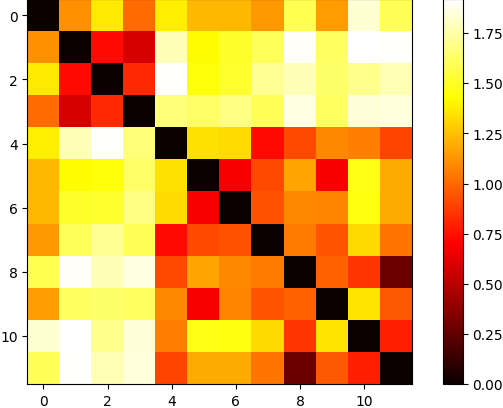
\includegraphics[width=\linewidth]{figures/syntetic_data/distance_matrix/SO3_signature_3.png}
        \caption{}
        \label{fig:classification-signature-level3-SO3}
    \end{subfigure}
    \hfill
    \begin{subfigure}{0.48\textwidth}
        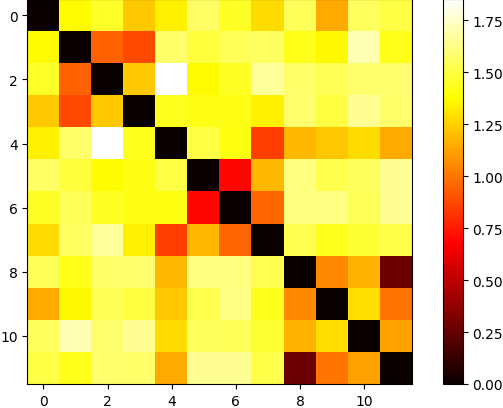
\includegraphics[width=\linewidth]{figures/syntetic_data/distance_matrix/SO3_signature_5.png}
        \caption{}
        \label{fig:classification-signature-level5-SO3}
    \end{subfigure}
    \vskip\baselineskip
    \begin{subfigure}{0.48\textwidth}
        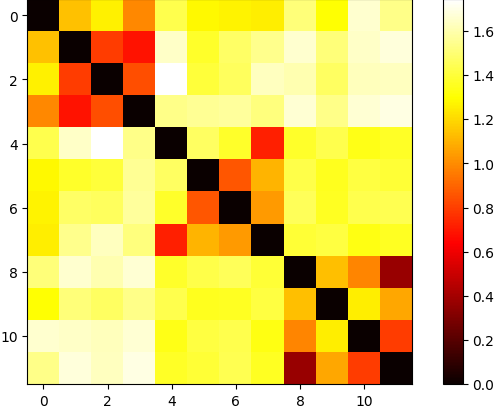
\includegraphics[width=\linewidth]{figures/syntetic_data/distance_matrix/SE3_signature_3.png}
        \caption{}
        \label{fig:classification-signature-level3-SE3}
    \end{subfigure}
    \hfill
    \begin{subfigure}{0.48\textwidth}
        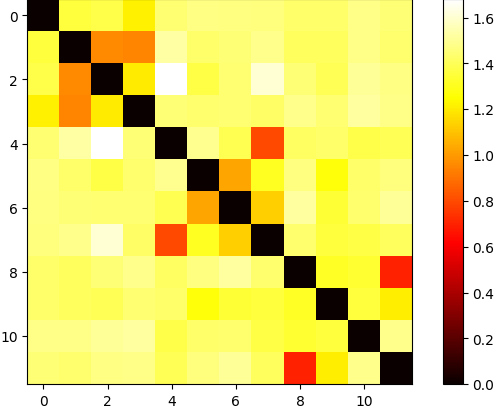
\includegraphics[width=\linewidth]{figures/syntetic_data/distance_matrix/SE3_signature_5.png}
        \caption{}
        \label{fig:classification-signature-level5-SE3}
    \end{subfigure}
    \caption[Classification using logarithmic signature on curves in \(\mathrm{SO}(3)\) and \(\mathrm{SE}(3)\)]{Distance matrices using the signature method for \(\mathrm{SO}(3)\) and \(\mathrm{SE}(3)\) at different truncation levels, visualized through the \(L^2\) norm between normalized signatures. Panels: (a) \(\mathrm{SO}(3)\), truncation level 3; (b) \(\mathrm{SO}(3)\), truncation level 5; (c) \(\mathrm{SE}(3)\), truncation level 3; (d) \(\mathrm{SE}(3)\), truncation level 5. These matrices illustrate the variation in signature-based classification accuracy across truncation levels.}
    \label{fig:classification-signature}
\end{figure}

\begin{figure}
    \centering
    \begin{subfigure}{0.48\textwidth}
        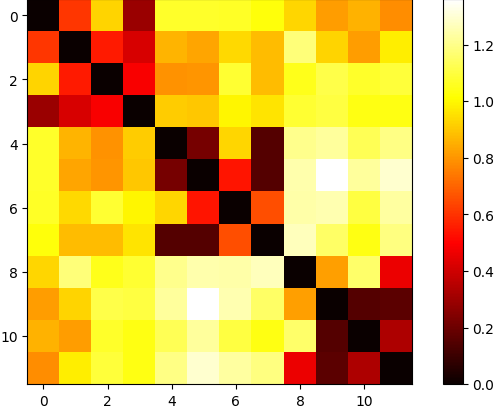
\includegraphics[width=\linewidth]{figures/syntetic_data/distance_matrix/SO3_3_signature_3.png}
        \caption{}
        \label{fig:classification-signature-level3-SO3-3}
    \end{subfigure}
    \hfill
    \begin{subfigure}{0.48\textwidth}
        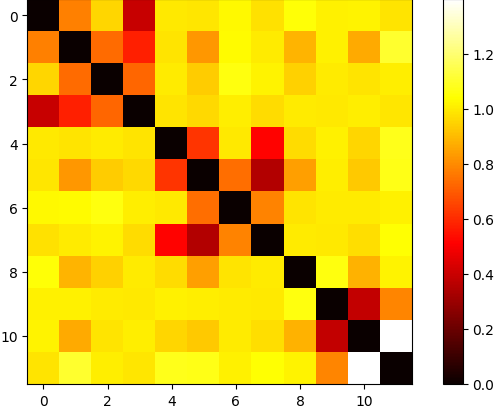
\includegraphics[width=\linewidth]{figures/syntetic_data/distance_matrix/SO3_3_signature_5.png}
        \caption{}
        \label{fig:classification-signature-level5-SO3-3}
    \end{subfigure}
    \vskip\baselineskip
    \begin{subfigure}{0.48\textwidth}
        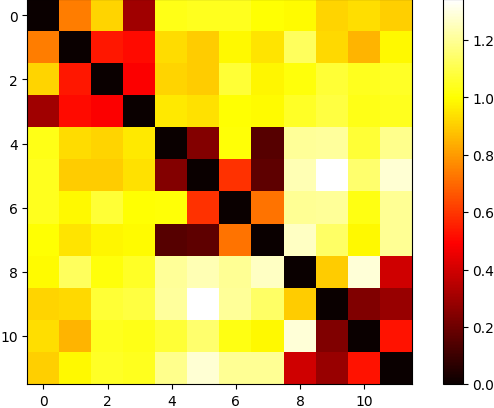
\includegraphics[width=\linewidth]{figures/syntetic_data/distance_matrix/SE3_3_signature_3.png}
        \caption{}
        \label{fig:classification-signature-level3-SE3-3}
    \end{subfigure}
    \hfill
    \begin{subfigure}{0.48\textwidth}
        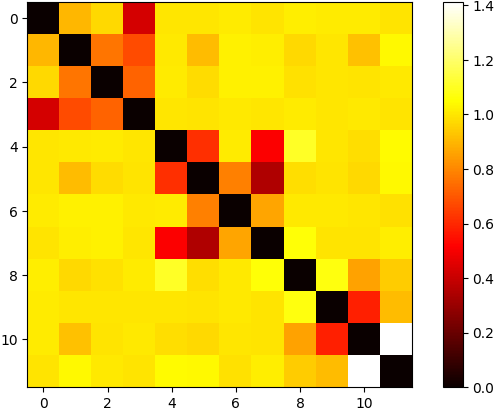
\includegraphics[width=\linewidth]{figures/syntetic_data/distance_matrix/SE3_3_signature_5.png}
        \caption{}
        \label{fig:classification-signature-level5-SE3-3}
    \end{subfigure}
    \caption[Classification using logarithmic signature on in \(\mathrm{SO}(3)^n\) and \(\mathrm{SE}(3)^n\)]{Distance matrices using the signature method for \(\mathrm{SO}(3)^3\) and \(\mathrm{SE}(3)^3\) at different truncation levels, visualized through the \(L^2\) norm between normalized signatures. Panels: (a) \(\mathrm{SO}(3)^3\), truncation level 3; (b) \(\mathrm{SO}(3)^3\), truncation level 5; (c) \(\mathrm{SE}(3)^3\), truncation level 3; (d) \(\mathrm{SE}(3)^3\), truncation level 5. These matrices illustrate the variation in signature-based classification accuracy across truncation levels.}
    \label{fig:classification-signature-3}
\end{figure}

In Figure \ref{fig:classification-signature}, it is evident that \(\mathrm{SE}(3)\) curves are more readily classified compared to \(\mathrm{SO}(3)\) curves, as shown by the more distinct clustering observed within the same geometric types. Increasing truncation levels in \(\mathrm{SO}(3)\) generally improves classification accuracy by incorporating more detailed information, resulting in a tighter grouping of curves with similar geometric characteristics. However, an interesting observation is made when the truncation level in \(\mathrm{SE}(3)\) is increased to 5: some curves from the same shape space unexpectedly exhibit large distances between them.

Figure \ref{fig:classification-signature-3} highlights the classification results for the spaces \(\mathrm{SO}(3)^n\) and \(\mathrm{SE}(3)^n\), which are notably promising. Distances within the same shape space remain low, indicating effective classification. Interestingly, classification performs better in \(\mathrm{SE}(3)^n\) than in \(\mathrm{SO}(3)^n\), demonstrating a superior ability to resolve geometric differences in these extended spaces. Similar to \(\mathrm{SE}(3)\), when the truncation level is increased to 5 in both \(\mathrm{SO}(3)^n\) and \(\mathrm{SE}(3)^n\), some curves from the same shape space begin to show significant distances between them.

These results highlight that the logarithmic signature is capable of distinguishing between curves of different shapes. By combining this with post-processing techniques, such as clustering, it may be possible to determine the shape of a curve based on its signature. However, the results also indicate that the choice of truncation level is crucial, as increasing the level may lead to unexpected results. Future work could explore the optimal truncation level for curve classification using the signature-based framework.

\subsection{Perturbation Analysis}
\label{subsec:perturbation-analysis-signature}

In this subsection, we investigate how the logarithmic signature-based distance metric (Equation \eqref{eq:signature-distance-metric}) behaves under perturbations. We utilize the curves \(c_i^\text{eq}\) and \(c_{i,i+1,i+2}^\text{eq}\) created in Subsection \ref{subsec:synthetic-data-generation}. To create a perturbed version of these curves, we solve the same differential equation \eqref{eq:diff-eq-synthetic}, but with timesteps perturbed by adding small, normally distributed noise. This results in the perturbed curves \(c_i^\epsilon\) and \(c_{i,i+1,i+2}^\epsilon\), with \(i \in \{1,2,3\}\) and \(i \in \{1,4,7\}\), respectively. We examine the effect of this perturbation on the signature-based distance metric by progressively reducing the standard deviation of the noise, performing this reduction 10 times. The results are shown in Figure \ref{fig:perturbation-analysis-signature}.

\begin{figure}
    \centering
    \begin{tikzpicture}
        \begin{loglogaxis}[
            width=0.8\textwidth,
            height=0.4\textwidth,
            xlabel={\(\epsilon\)},
            ylabel={\(d_{\mathcal{\text{sig}}_*}(c^\epsilon, c)\)},
            legend style={font=\small, at={(1.2,0.5)}, anchor=west},
            grid=major,
            legend pos=outer north east,
        ]
        
        \addplot [thick, red, solid] table [x=perturbation, y=c1, col sep=comma] {figures/syntetic_data/perturbation-analysis/signature-SO3.csv};
        \addlegendentry{\(\omega_0\)}

        \addplot [thick, blue, solid] table [x=perturbation, y=c2, col sep=comma] {figures/syntetic_data/perturbation-analysis/signature-SO3.csv};
        \addlegendentry{\(\omega_1\)}

        \addplot [thick, green, solid] table [x=perturbation, y=c3, col sep=comma] {figures/syntetic_data/perturbation-analysis/signature-SO3.csv};
        \addlegendentry{\(\omega_2\)}

        \addplot [thick, red, dashed] table [x=perturbation, y=c1, col sep=comma] {figures/syntetic_data/perturbation-analysis/signature-SE3.csv};
        \addlegendentry{\(\xi_0\)}

        \addplot [thick, blue, dashed] table [x=perturbation, y=c2, col sep=comma] {figures/syntetic_data/perturbation-analysis/signature-SE3.csv};
        \addlegendentry{\(\xi_1\)}

        \addplot [thick, green, dashed] table [x=perturbation, y=c3, col sep=comma] {figures/syntetic_data/perturbation-analysis/signature-SE3.csv};
        \addlegendentry{\(\xi_2\)}

        \logLogSlopeTriangle{0.7}{0.3}{0.2}{1}{black, dashed}
        
        \end{loglogaxis}
    \end{tikzpicture}
    \caption[Perturbation analysis plot of the logarithmic signature distance]{The signature based distance metric under perturbations in \(\mathrm{SO}(3)\) and \(\mathrm{SE}(3)\). The distance between the perturbed and non-perturbed curves is computed using the signature based distance metric. The curves are perturbed by adding a small normal distributed noise to the parameterization, where we halve the standard deviation, and the distance is computed 10 times.}
    \label{fig:perturbation-analysis-signature}
\end{figure}

We observe that as the perturbation size decreases, the signature-based distance metric also decreases. This indicates that the metric is robust to small perturbations, maintaining consistent performance even with minor noise in the parameterization of the curves.                      
\chapter{Analyzing Motion Capture Data}
\label{ch:analyzing-motion-capture-data}

In this chapter, we evaluate our shape analysis frameworks using real motion capture data from the CMU Motion Capture Library. This real-world test aims to validate the robustness and accuracy of our methods and explore the potential for combining them with post-processing techniques.

\section{Methodology}
\label{sec:motion-capture-data-methodology}

We utilize files from the CMU Motion Capture Library \cite{CarnegieMellonUniversity}, specifically XX.asf files and XX\_YY.amc files, where XX represents the subject (describing the skeleton or body of the performer) and YY represents the motion (the action performed). In Figure \ref{fig:skeleton}, we illustrate the skeleton structure, while Figure \ref{fig:jump_motion} shows a visual representation of a jump motion, combining the motion data with the skeleton structure.

Our study focuses on 44 motions, as listed in Table \ref{tab:shape_analysis_movements}: 9 'forward jumps', 9 'runs/jogs', 10 'walks', 9 'boxing' sequences, and 7 'stair climbing' sequences. These motions were chosen due to the availability of sufficient AMC files for each category. Each motion consists of 131 frames, matching the typical duration of a 'forward jump' motion, and all are recorded at a frame rate of 120 Hz. We ensured that the defining part of each motion was clearly visible, such as observing a punch in the boxing sequences.

The dataset includes ASF (Actor Skeleton File) and AMC (Actor Motion Capture Data) files. ASF files describe the skeleton structure and establish a base pose, while AMC files capture dynamic motion over time. We convert this data into joint-specific matrices, focusing on 23 joints to reduce noise from smaller joints such as thumbs, toes, and fingers. Each matrix contains rotational data for each timestep, resulting in a format of \((131, 23, 3, 3)\) representing (timestep, joint, rotation matrix).

Our hypothesis is that motions perceived as similar by humans (e.g., walking) are also mathematically similar, despite individual variations. To test this hypothesis, we will categorize the motions into five distinct groups and evaluate if our shape analysis framework accurately captures these similarities.

\begin{figure}[ht]
    \centering
    \begin{subfigure}[b]{0.4\textwidth}
        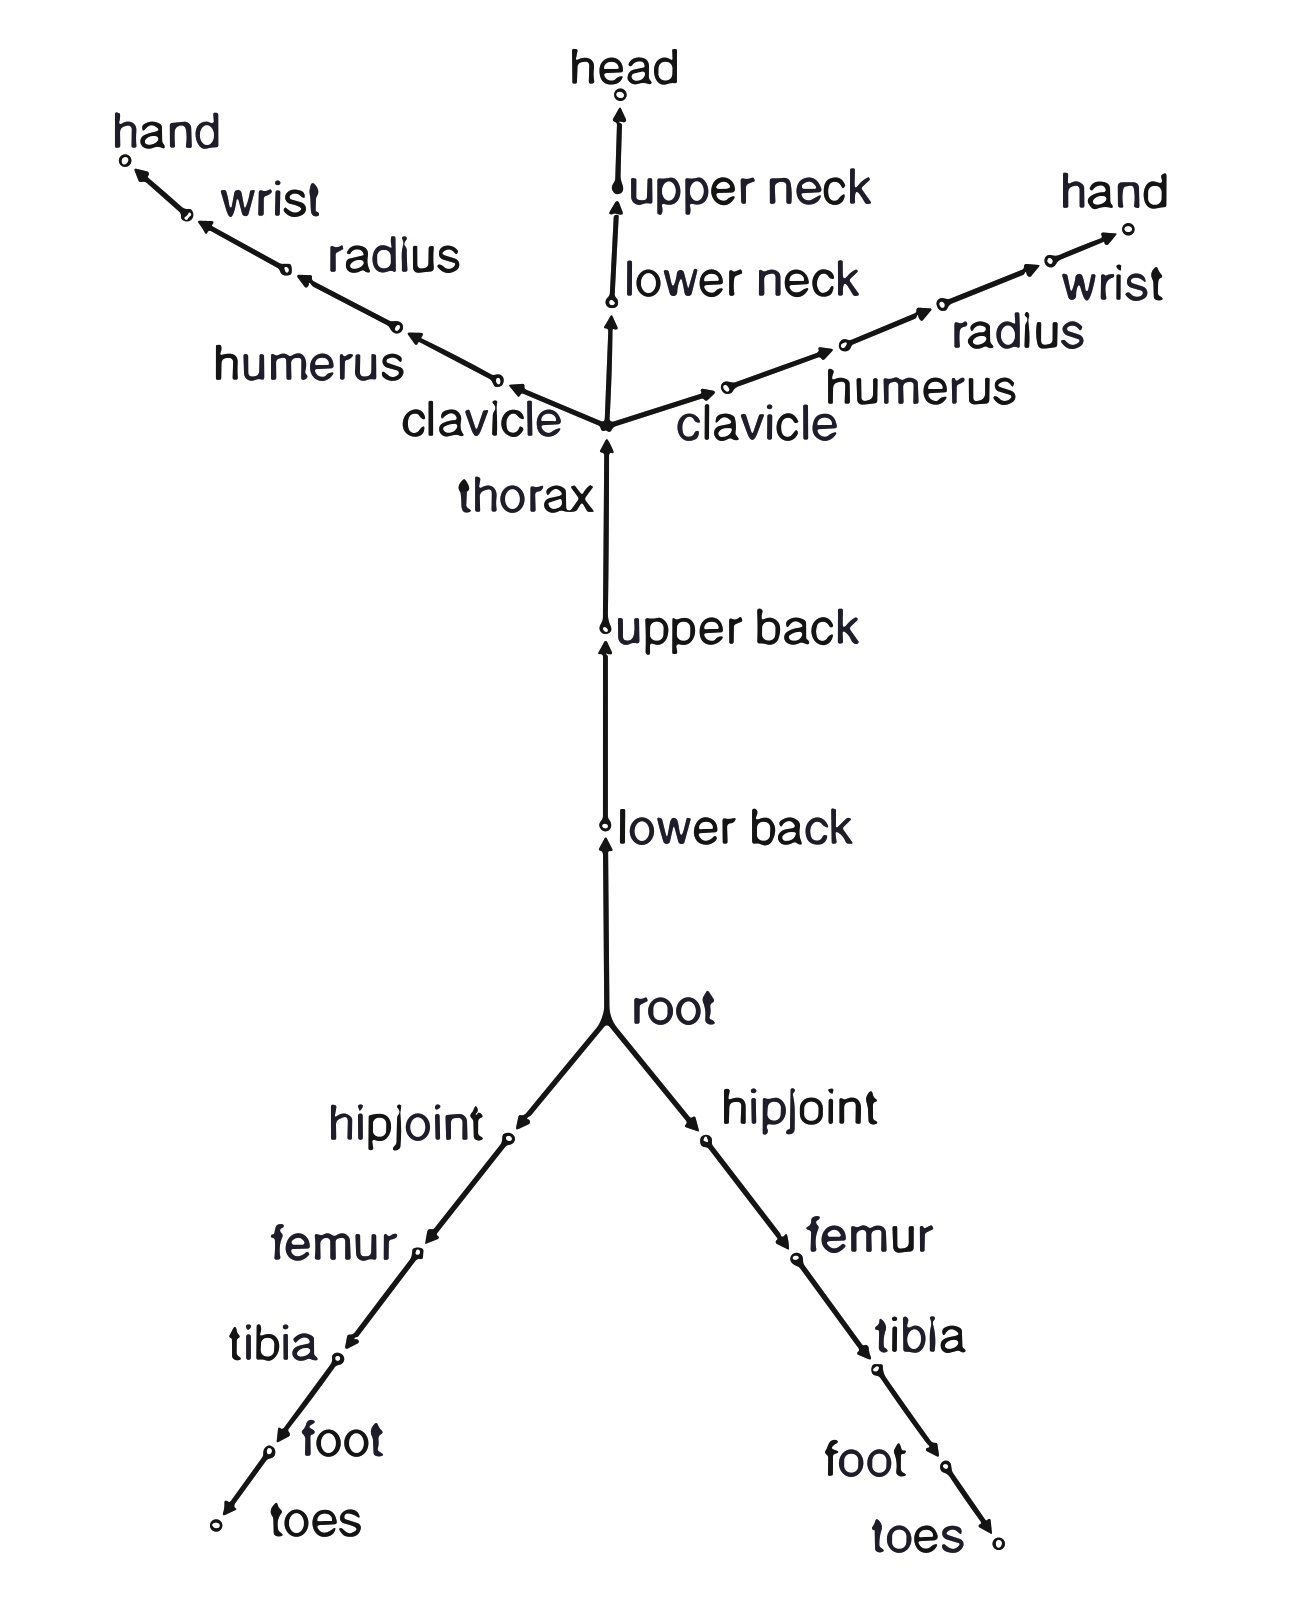
\includegraphics[width=\textwidth]{figures/motion-capture-data/Skeleton_image.png}
        \caption{}
        \label{fig:skeleton}
    \end{subfigure}
    \hfill
    \begin{subfigure}[b]{0.4\textwidth}
        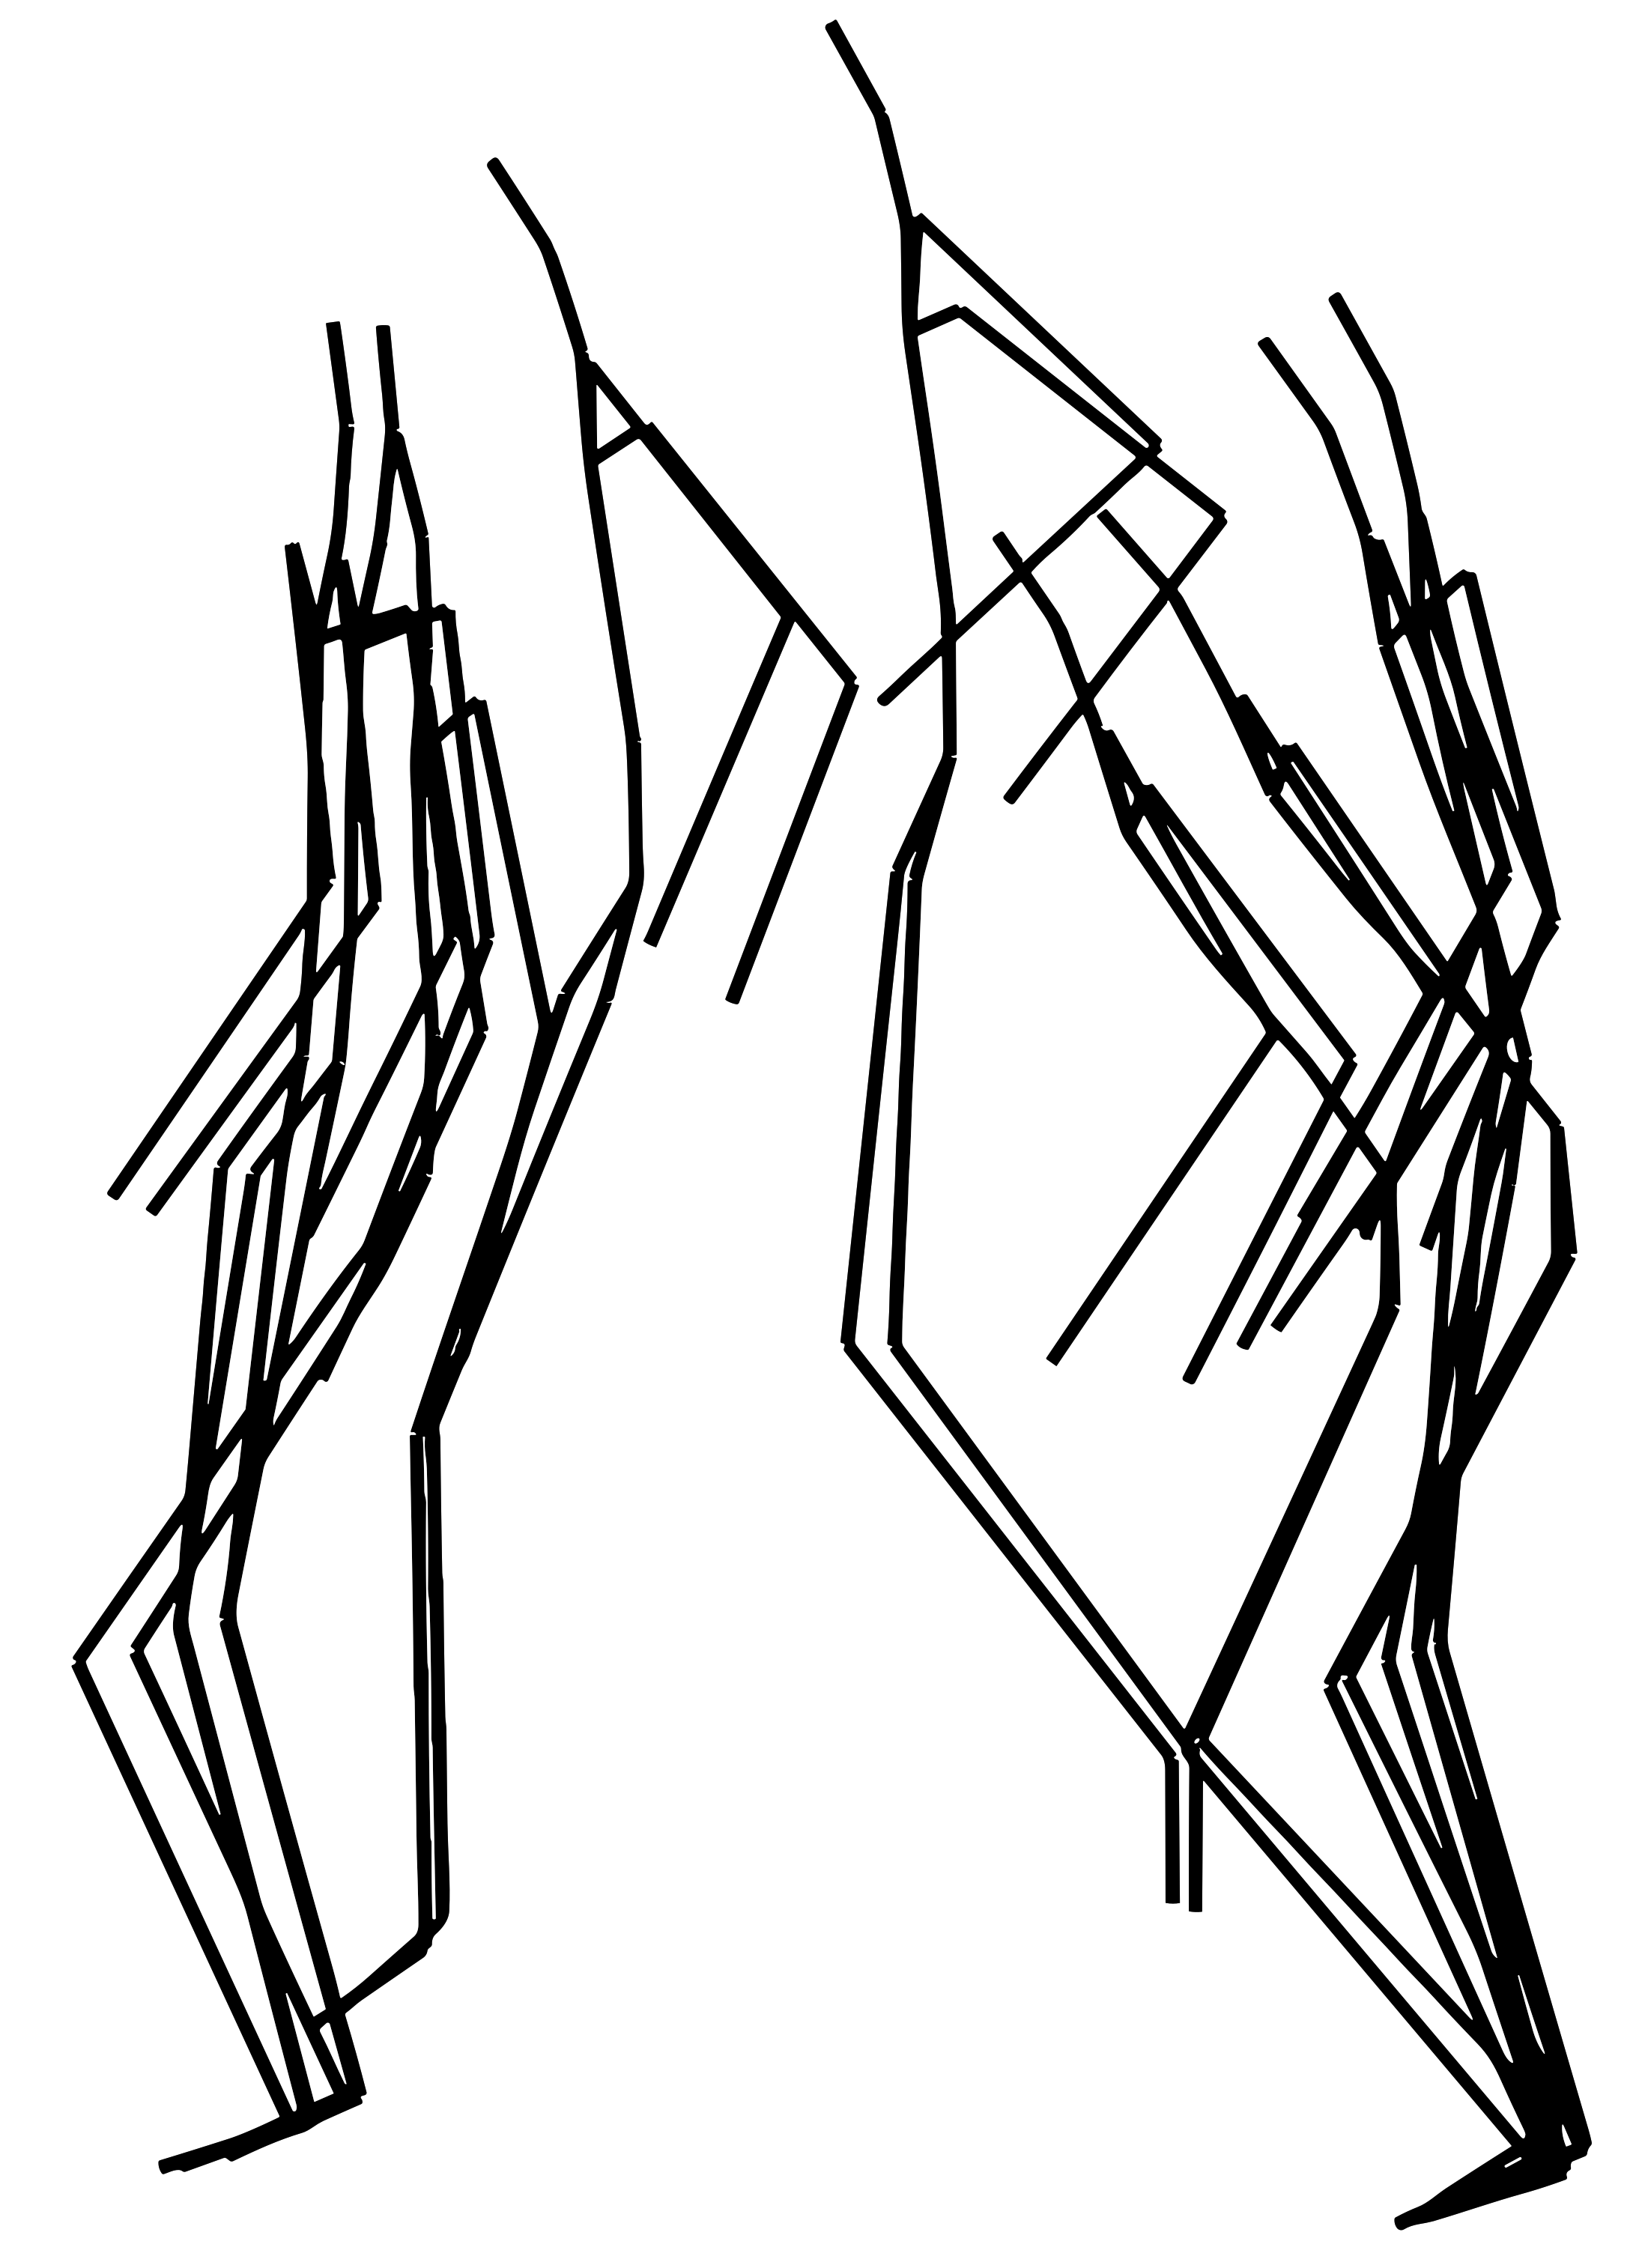
\includegraphics[height=0.3\textheight ,width=0.9\textwidth]{figures/motion-capture-data/Fig_16_05_trace_9_frames.png}
        \caption{}
        \label{fig:jump_motion}
    \end{subfigure}
    \caption[Visualization of the Motion Capture Data]{(a) Illustration of a human skeleton model for computer animation, showing the joint structure with labeled points. Adapted from \cite{bauerLandmarkGuidedElasticShape2015}. (b) Illustration of subject 16 motion 05, depicting one jump motion, 9 timeframes. Data for both illustrations from the CMU Graphics Lab Motion Capture Database \cite{CarnegieMellonUniversity}.}
    \label{fig:combined-motion-capture-figure}
\end{figure}

\section{Results}
\label{sec:motion-capture-data-results}

In this section, we utilize the frameworks from Chapter \ref{ch:optimal-reparameterization} and Chapter \ref{ch:signature-method} to analyze motion capture data. The objective is to evaluate the performance of these methods on real-world data and compare their results.

\subsection{Reparameterization with SRVT}
\label{subsec:motion-capture-data-reparameterization-srvt}

To find the distance between all motions in the dataset, we use the framework from Chapter \ref{ch:optimal-reparameterization}, which employs reparameterization of the SRVT (Square Root Velocity Transform) of the motions using Algorithm \ref{alg:optimal-reparam-dp} for optimal reparameterization. We then calculate the \(L^2\) distance between the SRVT of the motion and its reparameterized counterpart. This distance is stored in a distance matrix, where the diagonal is zero, as the distance between a motion and itself is zero.

The results are presented as a heatmap to show the unedited results, where the axes represent different motions, and the color indicates the distance between the two motions. These results are shown for various search depths (1, 4, and 10) to demonstrate that higher search depths yield improved outcomes. Ideally, the distance between similar motions should be smaller than the distance between dissimilar motions. Additionally, all motions from the same category should have similar distances to motions from other categories.

The motions are sorted before plotting the heatmap: motions 1-9 are forward jumps, 10-18 are runs/jogs, 19-28 are walks, 29-37 are boxing, and 38-44 are stair climbing. Thus, the heatmap should show blocks of the same color, where the blocks along the diagonal should have close to zero distance.

The results for different search depths using the SRVT method are shown in Figure \ref{fig:heatmaps-dynprog}. In \ref{fig:heatmaps-dynprog-1}, little structure is visible in the heatmap. It appears that the first two motions, "forward jump" and "run/jog," are dissimilar to each other, while the last three motions show some similarity. In \ref{fig:heatmaps-dynprog-4}, we observe four blocks along the diagonal, indicating that "forward jump," "run/jog," "walk," and "climbing stairs" are somewhat distinct. However, there are darker spots indicating some resemblance between walking and climbing stairs. In \ref{fig:heatmaps-dynprog-10}, a similar structure to that of search depth 4 is evident. It is not surprising that "walk" and "climbing stairs" are somewhat similar, as they involve similar motions, with one being on a flat surface and the other on stairs. It appears that boxing is the motion that is hardest for our method to distinguish from the others, which may be intrinsic to the motion itself or may be a limitation of the method.

\begin{figure}
    \centering
    \begin{subfigure}{\textwidth}
        \centering
        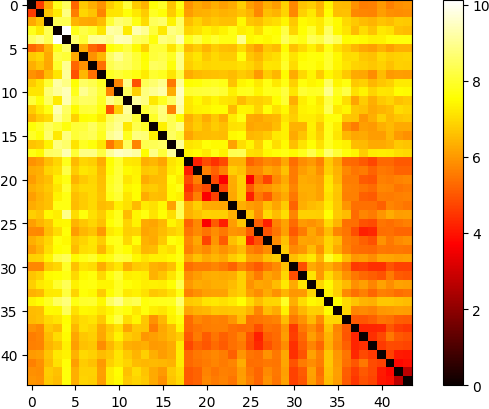
\includegraphics[width=0.53\textwidth]{figures/motion-capture-data/heatmaps/dynprog_1.png}
        \caption{}
        \label{fig:heatmaps-dynprog-1}
    \end{subfigure}
    \begin{subfigure}{\textwidth}
        \centering
        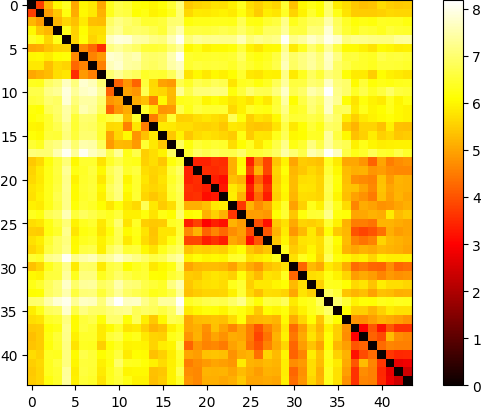
\includegraphics[width=0.53\textwidth]{figures/motion-capture-data/heatmaps/dynprog_4.png}
        \caption{}
        \label{fig:heatmaps-dynprog-4}
    \end{subfigure}
    \begin{subfigure}{\textwidth}
        \centering
        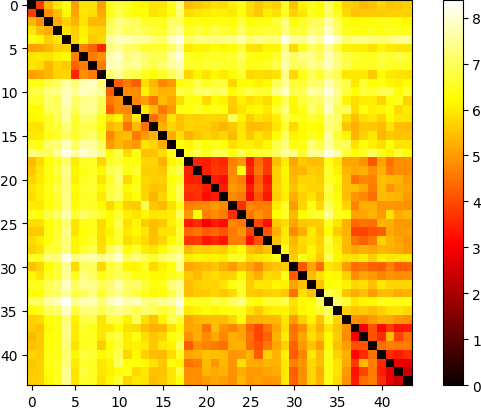
\includegraphics[width=0.53\textwidth]{figures/motion-capture-data/heatmaps/dynprog_10.png}
        \caption{}
        \label{fig:heatmaps-dynprog-10}
    \end{subfigure}
    \caption[Heatmap: Motion Capture Data Classification utilizing Reparameterization]{Heatmaps of the distance matrix from motion capture data, where the distance matrix was created by reparameterization using dynamic programming and search depths of: (a) 1, (b) 4, and (c) 10.}
    \label{fig:heatmaps-dynprog}
\end{figure}
\subsection{Logarithmic Signature}
\label{subsec:motion-capture-log-signature}

Another way to determine the shape space distance between two motions is to use the logarithmic signature method to find \(d_{\text{sig}_*}\) between all the curves, as defined in Equation \eqref{eq:signature-distance-metric}. We compute the logarithmic signature of each motion, normalize the signatures, and calculate the \(L^2\) norm of the difference between the normalized signatures. This distance is stored in a distance matrix, where the diagonal is zero since the distance between a motion and itself is zero.

\begin{figure}
    \centering
    \begin{subfigure}{\textwidth}
        \centering
        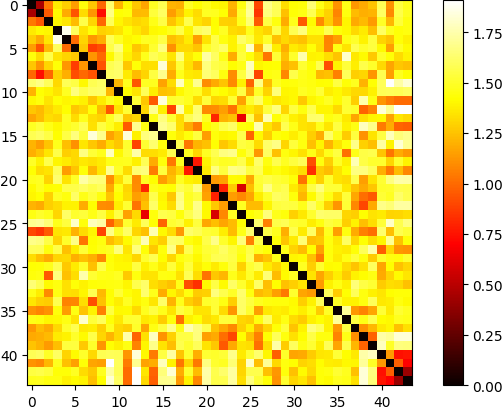
\includegraphics[width=0.53\textwidth]{figures/motion-capture-data/heatmaps/logsig_1.png}
        \caption{}
        \label{fig:heatmaps-logsig-1}
    \end{subfigure}
    \begin{subfigure}{\textwidth}
        \centering
        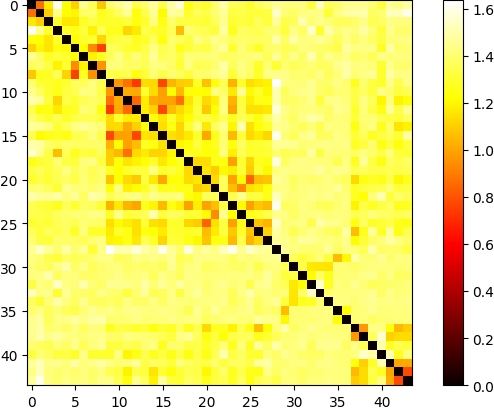
\includegraphics[width=0.53\textwidth]{figures/motion-capture-data/heatmaps/logsig_2.png}
        \caption{}
        \label{fig:heatmaps-logsig-2}
    \end{subfigure}
    \begin{subfigure}{\textwidth}
        \centering
        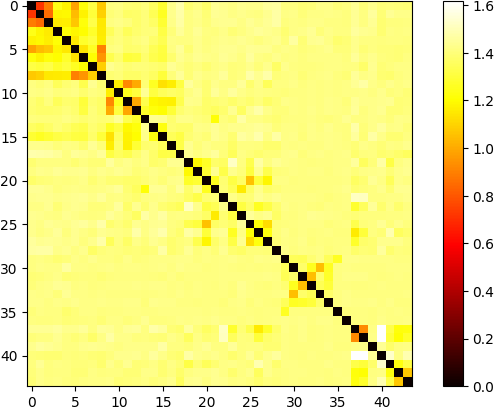
\includegraphics[width=0.53\textwidth]{figures/motion-capture-data/heatmaps/logsig_3.png}
        \caption{}
        \label{fig:heatmaps-logsig-3}
    \end{subfigure}
    \caption[Heatmap: Motion Capture Data Classification utilizing Logarithmic Signature]{Heatmaps of the distance matrix from motion capture data, where the distance matrix was created by the Logarithmic Signature and the \(L^2\) norm of these normalized signatures with truncation levels of: (a) 1, (b) 2, and (c) 3.}
    \label{fig:heatmaps-logsig}
\end{figure}

The results for three different truncation levels (1, 2, and 3) are shown in Figure \ref{fig:heatmaps-logsig}. In \ref{fig:heatmaps-logsig-1} there is significant noise, resembling Gaussian noise, indicating that it does not effectively distinguish between the motions. In \ref{fig:heatmaps-logsig-2} we see a block around "forward jump" and another block encompassing both "run/jog" and "walk" with a separate block forming at "climbing stairs". There is a significant distance between these and other motions. In \ref{fig:heatmaps-logsig-3} "forward jump" remains distinct, "run/jog" becomes distinct from "walk" and there are hints of "boxing" and "climbing stairs" being distinct.

These results show that higher truncation levels yield more detailed distinctions, enabling the method to better differentiate between various motions due to the increased nuanced information. Additionally, the logarithmic signature method highlights different aspects of the data compared to the reparameterization method, which is expected given the fundamental differences between the two approaches.
\newpage
\section{Post-Processing Techniques}
\label{sec:post-processing}

To enhance our analysis results and quantify the performance of our methods, we will explore various post-processing techniques. These techniques aim to improve the results and provide a deeper understanding of the data. We will employ methods such as Principal Component Analysis (PCA), classical Multidimensional Scaling (cMDS), and the k-medoids clustering algorithm. Additionally, we will utilize the silhouette score as an evaluation metric to assess the quality of the clustering.


\input{sections/motion-capture-data/post-processing/pca-cosine}
\input{sections/motion-capture-data/post-processing/k-medoids}
\input{sections/motion-capture-data/post-processing/cMDS}

\newpage
\input{sections/motion-capture-data/post-processing/silhouette-score}



\chapter{Conclusion}
\label{ch:conclusion}

This thesis explored two techniques for reparameterization: the fully discretized method using the Square Root Velocity Transform (SRVT) with dynamic programming, and the geodesic interpolation method, where optimal nodes were determined using Sequential Least Squares Programming (SLSQP). The primary focus was on dynamic programming. Both methods showed promise in achieving optimal reparameterizations and effectively discretizing curves based on their geometric shapes. These techniques were applied to compute the shape space distance between curves, utilizing the normalized logarithmic signature of curves for the same purpose.

We extended previous research by adapting these methodologies to the special Euclidean group (\(\mathrm{SE}(3)^n\)). Although we lacked real motion capture data for \(\mathrm{SE}(3)^n\), the methods were validated using synthetic data, indicating their potential utility.

Our framework was further expanded to include post-processing steps. Dimensionality reduction techniques, specifically Principal Component Analysis (PCA) and Classical Multi-Dimensional Scaling (cMDS), were employed, followed by clustering using K-Medoids. Silhouette scores were calculated to quantify the clustering quality, highlighting the importance of post-processing in enhancing the discriminative capability of our data.

Reparameterization proved particularly effective with motion capture data, discretizing five key moments identified in our study when post-processed. Although the logarithmic signature method was robust and faster, it was less effective. 

A problem was identified when using the logarithmic signature on \(\mathrm{SE}(3)^n\) data due to discrepancies between the matrix norm and the vector norm in its vectorized form, which biased the results towards translation over rotation. 

The post-processing phase was crucial in our analysis. By reducing the dimensionality of the data, we improved our ability to distinguish between different motions, facilitating effective clustering beyond mere visualization. This confirmed that data reduction enhances the classification of motion capture data. Silhouette scores further demonstrated the superiority of reparameterization utilizing SRVT over the logarithmic signature in terms of classification accuracy.

\newpage
\section*{Future Work}

Given the time and scope constraints of this thesis, several areas remain unexplored. Future research could focus on the following:

\begin{enumerate}
    \item \textbf{Classification on \(\mathrm{SE}(3)^n\) Data:} Exploring real motion capture data utilizing \(\mathrm{SE}(3)^n\) and attempting classification on such data could be valuable, as our tools show promise for these applications.
    
    \item \textbf{Mathematical Properties of Motions:} Investigate mathematical properties of motions, particularly \(\hat{u}(t)\), under the assumption that motions can be described as:
    \begin{equation*}
        \frac{d}{dt} g(t) = g(t)\hat u(t),
    \end{equation*}
    where we assume we can remove the parameterization, this aligns with our initial goals for reparameterization using geodesic interpolation.
    
    \item \textbf{Pre- and Post-Processing Analysis:} A detailed examination of both pre-processing and post-processing techniques could yield significant insights and improvements, given their highlighted importance in our study.
    
    \item \textbf{Semi-Discretized Methods on Motion Capture Data:} By utilizing semi-discretized methods to motion capture data we could achieve better optimal reparameterization and more accurate classification, as previous research has shown promising results for these methods.
    
    \item \textbf{Theoretical Analysis:} A more thorough analysis of the theoretical foundations of our methods would enhance understanding and potentially improve their application.
\end{enumerate}            

\chapter*{\bibname}
\begin{sloppypar}
\printbibliography[heading=none]
\end{sloppypar}

\appendix
\chapter{Additional Material}

\section{Inequality for Concave Functions}
\label{app:concave_inequality}

Consider a function \( f: \mathbb{R} \rightarrow \mathbb{R} \) that is concave, with the property that \( f(0) \geq 0 \). For any \( a, b \in \mathbb{R}^+ \), we aim to demonstrate the following inequality:

\begin{equation*}
f(a) + f(b) \geq f(a + b).
\end{equation*}

The definition of concavity for any function \( f \) stipulates that:

\begin{equation*}
f(\lambda x_1 + (1 - \lambda)x_2) \geq \lambda f(x_1) + (1 - \lambda)f(x_2),
\end{equation*}
for any \( x_1, x_2 \in \mathbb{R} \) and \( \lambda \in [0, 1] \). Applying this definition, we set \( x_1 = 0 \) and \( x_2 = a + b \), and examine two specific cases of \( \lambda \):

Let \( \lambda = \frac{a}{a + b} \). Then,

\begin{equation*}
\begin{aligned}
    f\left( \frac{a}{a+b} \cdot 0 + \frac{b}{a+b} \cdot (a+b) \right) 
    &\geq \frac{a}{a + b}f(0) + \frac{b}{a+b}f(a+b) \\
    f(b) &\geq \frac{b}{a+b}f(a+b),
\end{aligned}
\end{equation*}
where \( \frac{a}{a + b}f(0) \geq 0 \) due to the given condition that \( f(0) \geq 0 \).

Let \( \lambda = \frac{b}{a + b} \). Then,

\begin{equation*}
\begin{aligned}
    f\left( \frac{b}{a+b} \cdot 0 + \frac{a}{a+b} \cdot (a+b) \right) 
    &\geq \frac{b}{a + b}f(0) + \frac{a}{a+b}f(a+b) \\
    f(a) &\geq \frac{a}{a+b}f(a+b),
\end{aligned}
\end{equation*}
with \( \frac{b}{a + b}f(0) \geq 0 \) by the same premise.

Summing these inequalities yields:

\begin{equation}
f(a) + f(b) \geq \left( \frac{a}{a+b} + \frac{b}{a+b} \right)f(a+b) = f(a+b),
\label{eq:concave_inequality}
\end{equation}
thus confirming the asserted inequality.


%%%%%%%%%%%%%%%%%%%%%%%%%%%%%%%%%%%%%%%%%%%%%%%%%%%%%%%%%%%%%

\section{\texorpdfstring{\( q \)-Hölder Continuity of Power Norm Functions}{q-Hölder Continuity of Power Norm Functions}}
\label{app:q_holder_proof}

Consider the function \( f : \mathbb{R}^n \rightarrow \mathbb{R} \) defined by \( f(x) = \| x \|^q \) for a given \( q \in (0,1) \). We aim to demonstrate that \( f \) is \( q \)-Hölder continuous, i.e., there exists a constant \( C \in \mathbb{R}^+ \) such that for any \( x, y \in \mathbb{R}^n \), the following inequality holds:

\begin{equation}
\left| f(x) - f(y) \right| \leq C \| x - y \|^q.
\end{equation}

Using the results from \ref{app:concave_inequality}, we know that if \( f \) is concave and \( f(0) \geq 0 \), then for any \( a, b \in \mathbb{R}^+ \):

\begin{equation*}
f(a) + f(b) \geq f(a + b).
\end{equation*}

In this case, since \( f(z) = z^q \) is concave for \( z \geq 0 \), we apply the definition of concavity directly. Assume without loss of generality that \( \| x \| \geq \| y \| \). Then,

\begin{equation*}
\left| \| x \|^q - \| y \|^q \right| = \| x \|^q - \| y \|^q.
\end{equation*}

By the concavity of \( f(z) = z^q \), we have:

\begin{equation*}
\left( \| y \| + \| x - y \| \right)^q \leq \| y \|^q + \| x - y \|^q.
\end{equation*}

Thus,

\begin{equation*}
\| x \|^q = \left( \| y + (x - y) \| \right)^q \leq \left( \| y \| + \| x - y \| \right)^q \leq \| y \|^q + \| x - y \|^q.
\end{equation*}

Therefore,

\begin{equation*}
\| x \|^q - \| y \|^q \leq \| x - y \|^q.
\end{equation*}

By symmetry, if \( \| y \| \geq \| x \| \), the same argument applies. Hence, we conclude:

\begin{equation*}
\left| f(x) - f(y) \right| = \left| \|x\|^q - \|y\|^q \right| \leq \|x - y\|^q,
\end{equation*}

confirming the \( q \)-Hölder continuity of \( f \) with constant \( C = 1 \).

%%%%%%%%%%%%%%%%%%%%%%%%%%%%%%%%%%%%%%%%%%%%%%%%%%%%%%%%%%%%%


\section{\texorpdfstring{$\alpha$}{alpha}-Hölder Continuity}
\label{app:alpha_holder_proof}

Consider the function \( V : \mathbb{R}^n \rightarrow \mathbb{R}^n \) defined by \( V(x) = x \|x\|^{\alpha - 1} \) for \( 0 < \alpha \leq 1 \). We aim to demonstrate that \( V \) is \( \alpha \)-Hölder continuous, i.e., there exists a constant \( C \in \mathbb{R}^+ \) such that for any \( x, y \in \mathbb{R}^n \):

\begin{equation*}
    \left\| x\|x\|^{\alpha-1} - y\|y\|^{\alpha-1} \right\| \leq C \|x - y\|^{\alpha}.
\end{equation*}

Using the results from \ref{app:q_holder_proof}, we know that if \( f(x) = \|x\|^q \) is \( q \)-Hölder continuous, then

\begin{equation*}
\left| \|x\|^q - \|y\|^q \right| \leq \|x - y\|^q,
\end{equation*}
for any \( x, y \in \mathbb{R}^n \) and \( q \in (0, 1) \). Applying this result, we proceed as follows:

\begin{equation*}
    \begin{aligned}
        \left\| x \|x\|^{\alpha - 1} - y \|y\|^{\alpha - 1} \right\| 
        &= \left\| x \|x\|^{\alpha - 1} - \underbrace{\|x\|\frac{y}{\|y\|} + \|x\|\frac{y}{\|y\|}}_{=0} - y \|y\|^{\alpha - 1} \right\| \\
        &\leq \left\| x \|x\|^{\alpha - 1} - \|x\|^\alpha \frac{y}{\|y\|} \right\| + \left\| \|x\|^\alpha \frac{y}{\|y\|} - y \|y\|^{\alpha - 1} \right\| \\
        &= \left\|\|x\| \frac{\|x\|^\alpha}{\|x\|} - \|x\|^\alpha \frac{y}{\|y\|} \right\| + \left\|\|x\|^\alpha \frac{y}{\|y\|} - \|y\|^\alpha \frac{y}{\|y\|} \right\| \\
        &= \|x\|^{\alpha - 1} \left\| x - \underbrace{y + y}_{=0} - \|x\| \frac{y}{\|y\|} \right\| + \left| \|x\|^\alpha - \|y\|^\alpha \right| \left\| \frac{y}{\|y\|} \right\| \\
        &= \|x\|^{\alpha - 1} \underbrace{\left\| x - y + y \frac{\|y\| - \|x\|}{\|y\|} \right\|}_{i} + \left| \|x\|^\alpha - \|y\|^\alpha \right|.
    \end{aligned}
\end{equation*}

We can bound \((i)\) as follows:
\begin{equation*}
    \begin{aligned}
        \left\| x - y + y \frac{\|y\| - \|x\|}{\|y\|} \right\| 
        &\leq \left\| x - y \right\| + \left\| y \frac{\|y\| - \|x\|}{\|y\|} \right\| \\
        &= \left\| x - y \right\| + \left| \|y\| - \|x\| \right| \\ 
        &\leq 2\left\| x - y \right\|.
    \end{aligned}
\end{equation*}

Substituting this bound back into the inequality, we have:

\begin{equation*}
        \|x\|^{\alpha - 1} \left\| x - y + y \frac{\|y\| - \|x\|}{\|y\|} \right\| + \left| \|x\|^\alpha - \|y\|^\alpha \right| 
        \leq 2 \|x\|^{\alpha - 1} \|x - y\| + \left| \|x - y\|^\alpha \right| 
\end{equation*}

Assuming without loss of generality that \(\|x\| \geq \|y\| > 0\), we consider two cases:

If \(\|x-y\| \leq \|x\|\), then:
\begin{equation*}
    \|x\|^{\alpha - 1}  \leq \|x-y\|^{\alpha - 1},
\end{equation*}
such that 
\begin{equation*}
    \begin{aligned}
        2 \|x\|^{\alpha - 1} \|x - y\| + \|x - y\|^\alpha 
        &\leq 2 \|x-y\|^{\alpha - 1} \|x - y\| + \|x - y\|^\alpha  \\
        &= 2 \|x-y\|^{\alpha} + \|x - y\|^\alpha \\
        &= 3 \|x-y\|^{\alpha}.
    \end{aligned}
\end{equation*}

If \(\|x-y\| > \|x\|\), then:
\begin{equation*}
    \|x-y\| \leq \|x\| + \|y\| \leq 2\|x\|,
\end{equation*}
such that:
\begin{equation*}
    \begin{aligned}
        2 \|x\|^{\alpha - 1} \|x - y\| + \|x - y\|^\alpha 
        &\leq 2 \|x\|^{\alpha - 1} 2\|x\| + \|x - y\|^\alpha \\
        &\leq 4 \|x - y\|^{\alpha} + \|x - y\|^\alpha \\
        &= 5 \|x - y\|^{\alpha}.
    \end{aligned}
\end{equation*}

Thus, we have shown that:
\begin{equation*}
    \left\| x \|x\|^{\alpha - 1} - y \|y\|^{\alpha - 1} \right\| \leq 5 \|x - y\|^{\alpha},
\end{equation*}

which means that \( V \) is \( \alpha \)-Hölder continuous with \( C = 5 \).
\chapter{Movement data}

\section{Table of Movement Data}

\begin{longtable}{cccc}
    \caption[List of Movements Used in Shape Analysis]{Table list of the motions used in the shape analysis. The movements are taken from the CMU Graphics Lab Motion Capture Database \cite{CarnegieMellonUniversity}.} \label{tab:shape_analysis_movements} \\
    \hline
    Movement Type & File & Start & End \\
    \hline
    \endfirsthead
    \multicolumn{4}{c}%
    {\tablename\ \thetable\ -- \textit{Continued from previous page}} \\
    \hline
    Movement Type & File & Start & End \\
    \hline
    \endhead
    \hline \multicolumn{4}{r}{\textit{Continued on next page}} \\
    \endfoot
    \hline
    \endlastfoot
    Forward Jump & 16\_05.amc & 90 & 220 \\
    Forward Jump & 16\_06.amc & 200 & 330 \\
    Forward Jump & 16\_07.amc & 200 & 330 \\
    Forward Jump & 16\_09.amc & 240 & 370 \\
    Forward Jump & 16\_10.amc & 260 & 390 \\
    Forward Jump & 13\_11.amc & 190 & 320 \\
    Forward Jump & 13\_13.amc & 160 & 290 \\
    Forward Jump & 13\_19.amc & 205 & 335 \\
    Forward Jump & 13\_32.amc & 125 & 255 \\
    Run/Jog & 16\_45.amc & 0 & 130 \\
    Run/Jog & 16\_46.amc & 0 & 130 \\
    Run/Jog & 35\_26.amc & 0 & 130 \\
    Run/Jog & 35\_22.amc & 0 & 130 \\
    Run/Jog & 16\_35.amc & 0 & 130 \\
    Run/Jog & 16\_36.amc & 0 & 130 \\
    Run/Jog & 35\_18.amc & 0 & 130 \\
    Run/Jog & 02\_03.amc & 0 & 130 \\
    Run/Jog & 16\_56.amc & 0 & 130 \\
    Walk & 16\_16.amc & 0 & 130 \\
    Walk & 35\_12.amc & 0 & 130 \\
    Walk & 16\_58.amc & 0 & 130 \\
    Walk & 35\_32.amc & 0 & 130 \\
    Walk & 35\_11.amc & 0 & 130 \\
    Walk & 16\_21.amc & 0 & 130 \\
    Walk & 16\_22.amc & 0 & 130 \\
    Walk & 16\_15.amc & 40 & 170 \\
    Walk & 16\_31.amc & 40 & 170 \\
    Walk & 16\_47.amc & 40 & 170 \\
    Boxing & 13\_17.amc & 30 & 160 \\
    Boxing & 13\_18.amc & 30 & 160 \\
    Boxing & 14\_01.amc & 40 & 170 \\
    Boxing & 14\_02.amc & 40 & 170 \\
    Boxing & 14\_03.amc & 80 & 210 \\
    Boxing & 15\_13.amc & 80 & 210 \\
    Boxing & 17\_10.amc & 80 & 210 \\
    Boxing & 15\_04.amc & 22200 & 22330 \\
    Boxing & 15\_05.amc & 22400 & 22530 \\
    Climb Stairs & 13\_35.amc & 200 & 330 \\
    Climb Stairs & 13\_36.amc & 230 & 360 \\
    Climb Stairs & 13\_37.amc & 220 & 350 \\
    Climb Stairs & 13\_38.amc & 220 & 350 \\
    Climb Stairs & 14\_21.amc & 220 & 350 \\
    Climb Stairs & 14\_22.amc & 220 & 350 \\
    Climb Stairs & 14\_23.amc & 220 & 350 \\
\end{longtable}



\end{document}
